\documentclass[a4paper,12pt,brazil,oneside]{book}

\usepackage{amssymb}                        %%% para simbolo de 'marca registrada'
\usepackage[brazil]{varioref}               %%% referencias com página \vref
\usepackage[sf,bf,compact,topmarks,calcwidth,pagestyles]{titlesec} %%% definir títulos de seção
\usepackage{amsmath,amsfonts,amstext,amsthm,textcomp}
\usepackage{fancybox}                       %%% boxes
\usepackage[dvipsnames,usenames]{color}                          %%% Cores de fonte e fundo
\usepackage[dvipsnames,usenames]{xcolor}
\usepackage{colortbl}                       %%% Cores em tabelas
\usepackage{rotating}
\usepackage{fancyvrb}                       %%% Inclusão de texto usando VerbatimInput
\usepackage{bookman}                        %%% Fonte de Letras
\usepackage{enumerate}
\usepackage{lettrine}
\usepackage{minted}	
\usepackage{caption}
\usepackage{framed}
\usepackage{enumitem}

%\usepackage{listings}
%\lstset{
%  numbers=left,
%  numberstyle=\tiny,
%  mathescape=true,
%  frame=single,
%  stepnumber=1,
%%  basicstyle=\scriptsize, % fontes menores nos codigos
%  keywordstyle=\ttfamily,
%  identifierstyle=\ttfamily, % \bfseries negrito nos codigos
%  commentstyle=\ttfamily
%}
\usepackage{pstricks} % listings color: black!50!red

\usepackage{listings}
\lstset{
	numbers=left,
	stepnumber=1,
	firstnumber=1,
	numberstyle=\tiny,
	mathescape=true,
	extendedchars=true,
	breaklines=true,
	frame=single,
	basicstyle=\footnotesize,
%	basicstyle=\scriptsize,
	stringstyle=\ttfamily,
% 	moredelim=*[l][\itshape]{||},%
	showstringspaces=false,
	float=h,
}
\lstdefinelanguage{lalp} {
  sensitive=true,
  keywordstyle={\color{black!50!green}\ttfamily\bfseries},
  keywords={const, typedef, fixed, in, out, counter, when, block_ram, delay_op, mult_op_s, add_reg_op_s},
  otherkeywords={<-},
  otherkeywords={@},
  commentstyle={\color{black!50!red}\itshape},
  morecomment=[l]{//}, 
  morecomment=[s]{/*}{*/},
}
\lstdefinelanguage{ican} {
  sensitive=true,
  keywordstyle={\color{black!50!red}\ttfamily\bfseries},
  keywords={array, begin, boolean, by, case, character, default, do, each, elif, else, end, enum, esac, false, fi, for, goto, if, in, inout, integer, nil, od, of, out, procedure, real, record, repeat, return, returns, sequence, set, to, true, until, where, while},
  commentstyle={\color{black!50!green}\itshape},
  morecomment=[l]{||},
  literate={{(X)}{$\times$}1 {(E)}{$\in$}1 {(U)}{$\cup$}1 {(N)}{$\cap$}1 {(<)}{$\langle$}1 {(>)}{$\rangle$}1 {->}{$\rightarrow$}2 {<\-}{$\leftarrow$}2 {=}{$=$}1 {>}{$>$}1 {<}{$<$}1 {!=}{$\neq$}1 {>=}{$\ge$}1 {<=}{$\le$}1}
}

\renewcommand\listingscaption{Algoritmo}
\renewcommand\listoflistingscaption{Lista de Algoritmos}


\usepackage[english,brazil]{babel}
\usepackage[utf8]{inputenc}
\usepackage[T1]{fontenc}
\usepackage{times}
\usepackage{graphicx,xr}
\usepackage{subfigure}
\usepackage{longtable}
\usepackage{setspace}
\usepackage{multirow}
\usepackage{rotating}
\usepackage{indentfirst}
\usepackage{xspace}
\usepackage[sort]{natbib}
\usepackage[a4paper,top=30mm,bottom=20mm,left=30mm,right=20mm]{geometry}

\usepackage{hyperref}
\hypersetup{
%  backref, %omitir na versão final
  pdfsubject =	{...},
  pdftitle =	{...},
  pdfkeywords = {...},
  pdfauthor =	{Ricardo Menotti, Daniel Lucrédio, ...},
  colorlinks =	{true}, %true na versão final
  linkcolor =	{black!50!blue},
  citecolor =	{black!50!blue},
  urlcolor =	{black!50!blue},
}

\exhyphenpenalty = 10000

\onehalfspace

\hyphenation{es-ta-be-le-ci-das a-tu-al-men-te Simple-Scalar-ARM}

\newcommand{\up}[1]{\raisebox{1.5ex}[0pt]{#1}}

\newcommand{\bi}{\begin{itemize}}
\newcommand{\ei}{\end{itemize}}
\newcommand{\be}{\begin{enumerate}}
\newcommand{\ee}{\end{enumerate}}

\definecolor{Gray}{gray}{0.9}

% using \autoref{} instead
%\newcommand{\reffig}[1]{Figura~\ref{fig:#1}}
%\newcommand{\reftab}[1]{Tabela~\ref{tab:#1}}
%\newcommand{\refcha}[1]{Capítulo~\ref{cha:#1}}
%\newcommand{\refses}[1]{Seção~\ref{ses:#1}}
%\newcommand{\refsub}[1]{Subseção~\ref{sub:#1}}
%\newcommand{\refape}[1]{Apêndice~\ref{ape:#1}}
%\newcommand{\refcod}[1]{Código~\ref{cod:#1}}
\newcommand{\subfigureautorefname}{\figureautorefname}

\newcommand{\cha}[2]{\chapter{#2}\label{cha:#1}} %\thispagestyle{empty}
\newcommand{\ses}[2]{\section{#2}\label{ses:#1}}
\newcommand{\sub}[2]{\subsection{#2}\label{sub:#1}}
\newcommand{\ape}[2]{\chapter{#2}\label{ape:#1}} %\thispagestyle{empty}

\newcommand{\figsim}[2]{
\begin{figure}[!ht]
  \centering
  \includegraphics[width=\textwidth]{../figuras/#1.jpg}
  \caption{#2}
  \label{fig:#1}
\end{figure}
}

\newcommand{\ew}[1]{\selectlanguage{english}\emph{#1}\selectlanguage{brazil}}
%\newcommand{\ew}[1]{\emph{#1}}

\renewcommand{\bibname}{Referências Bibliográficas}

\setcounter{secnumdepth}{2}

\setcounter{tocdepth}{2}

\pagestyle{empty}

%\font\numberfont= goxi2074 scaled 2000      %%% Fonte para o Número do Capítulo
\font\numberfont= pzcmi scaled 6500      %%% Fonte para o Número do Capítulo

                                            %%% redefine o formato do título
\titleformat{\chapter}[display]
  {\normalfont\Large\sffamily
  }
  {
   \rule[32pt]{.7\linewidth}{4pt}
   \hspace{-10pt}
   \shadowbox{
   \begin{minipage}{.18\linewidth}
     \begin{center}
       \textsc{\Large\chaptertitlename}\\
       \vspace{1ex}
       {\numberfont \thechapter}\\
       \vspace{1ex}
     \end{center}
   \end{minipage}}
  }
  {0pt}
  {\filcenter
   \Huge
   }
  [\hfill\rule{.8\textwidth}{0.75pt}\\
     \vskip-1.8ex\hfill\rule{.7\textwidth}{2pt}]


\newpagestyle{body}{ %[\small\sffamily]{
\headrule

\sethead[\thepage][][\ifthechapter{\thechapter\quad}{} \textsl{\chaptertitle}]%
          {\ifthechapter{\thechapter\quad \textsl{\chaptertitle}}{\textsl{\chaptertitle}}}{}{\thepage}


}

\newpagestyle{misc}{
  \headrule
  \sethead{\textsl{\chaptertitle}}{}{\thepage}
  \setfoot{}{}{}
}

\font\largefont= pzcmi scaled 6500

\newcommand{\versal}[1]{{\noindent
    \setbox0\hbox{\largefont #1 }%
    \count0=\ht0                   % height of versal
    \count1=\baselineskip          % baselineskip
    \divide\count0 by \count1      % versal height/baselineskip
    \dimen1 = \count0\baselineskip % distance to drop versal
    \advance\count0 by 1\relax     % no of indented lines
    \dimen0=\wd0                   % width of versal
    \global\hangindent\dimen0      % set indentation distance
    \global\hangafter-\count0      % set no of indented lines
    \hskip-\dimen0\setbox0\hbox to\dimen0{\raise-\dimen1\box0\hss}%
    \dp0=0in\ht0=0in\box0}}


%%%  define linha mais grossa para tabelas

\newdimen\arrayruleHwidth
\setlength{\arrayruleHwidth}{2pt} \makeatletter
\def\Hline{\noalign{\ifnum0=`}\fi\hrule \@height \arrayruleHwidth
\futurelet \@tempa\@xhline} \makeatother

\definecolor{mygreen}{rgb}{0.1, 0.6, 0.2}


\title{Título}

\begin{document}
\selectlanguage{brazil}

%!TEX root = ios.tex

\begin{center}
%\normalfont\sffamily

\begin{minipage}[c]{\textwidth}
  \parbox[c]{3cm}{
      \begin{flushright}
      
\includegraphics[width=.25\textwidth]{../figuras/LogoUfscar}
      \end{flushright}
  }
  \parbox[c]{12cm}
    {
      \begin{center}
      \textbf{\Large Universidade Federal de São Carlos}

      \vspace{0.07cm}

      \textbf{\large Centro de Ciências Exatas e de Tecnologia}

      \vspace{0.07cm}

      \textbf{\large Departamento de Computação}
      \vspace{0.07cm}
      \end{center}
    }
\end{minipage}

\vspace{-0.5cm}
\rule{7.5cm}{0.03pc}{\tiny $_\diamondsuit$}\rule{7.5cm}{0.03pc}

\vspace*{20ex}

\textbf{\Large {Introdução às tecnologias para desenvolvimento de \\ aplicações em plataformas móveis iOS}} \\
\large{ Processo: \textbf{23112.003595/2012-35}}

\vspace*{5ex}

{\Large{ Coordenadores:  }} \\
\textbf{\Large{ Ricardo Menotti}} \\
\textbf{\Large{ Daniel Lucrédio}}

\vspace*{5ex}

{\Large{ Autor/Bolsista:  }}  \\
\textbf{\Large{ Régis Magno Zangirolami } } 
%\textbf{\Large{ Matheus Fernando Finatti }}  \\

\vspace*{10ex}

\textbf{\large São Carlos - SP, \today}

\vspace*{5ex}


\includegraphics[width=.25\textwidth]{../figuras/LogoDC} \hfill

\includegraphics[width=.25\textwidth]{../figuras/LogoProEx}

\end{center} 

\pagestyle{empty}

\clearpage

\selectlanguage{brazil}
\onehalfspace

\pagestyle{plain}
\pagenumbering{roman}

\chapter*{Sobre este documento}
\addcontentsline{toc}{chapter}{Sobre}
Os seguintes autores contribuíram para a elaboração deste material, a revisão indicada é a última realizada por cada um deles:
  \begin{itemize}
	\item Caio Cesar Almeida Pegoraro \dotfill r112
    \item Régis Magno Zangirolami \dotfill r77
  \end{itemize}
O código fonte do material, bem como de todos os exemplos usados, encontra-se disponível em \href{http://mobile.dc.ufscar.br/}{http://mobile.dc.ufscar.br/}.
\thispagestyle{empty}

\chapter*{Resumo}
\addcontentsline{toc}{chapter}{Resumo}

\begin{singlespace}
Esse material didático oferece uma visão geral de como programar para o sistema móvel iOS e utilizar suas APIs nativas na criação de aplicativos. O material tentará cobrir desde o básico, como a configuração do ambiente de desenvolvimento, criação de layouts básicos e complexos, estrutura geral de um aplicativo e, finalmente, apresentar a programação de aplicativos mais complexos que utilizam APIs nativas.

O objetivo é fornecer noções sobre como utilizar as ferramentas do iOS, introduzir os conceitos sem entrar em detalhes aprofundados do sistema operacional e assim disponibilizar uma visão básica sobre o assunto.
Após a leitura desse material e realização da prática o leitor deverá estar preparado para construir seus próprios aplicativos nativos, e poderá até monetizá-los se desejar.
\end{singlespace}
\thispagestyle{empty}


\setcounter{tocdepth}{1} % 0 capítulos, 1 seções, 2 subseções
\tableofcontents
\thispagestyle{empty}

\listoffigures
\addcontentsline{toc}{chapter}{Lista de Figuras}
\thispagestyle{empty}

\listoftables
\addcontentsline{toc}{chapter}{Lista de Tabelas}
\thispagestyle{empty}

\listoflistings
\thispagestyle{empty}

%\chapter*{Lista de Abreviaturas}
%\addcontentsline{toc}{section}{Lista de Abreviaturas}
%\begin{longtable}{ll}
%\end{longtable}

\usemintedstyle{perldoc}

\thispagestyle{empty}

\doublespace
%\onehalfspace
%\singlespace

\pagestyle{body}
\pagenumbering{arabic}

%%%%%%%%%%%%%%%%%%%%%%%%%%%%%%%%%%%%%%%%%%%%%%%%%%%%%%%%%%%%%%%%%%%%%%%%%%%%%%%%
\cha{introducao}{Introdução}

Este material tem a intenção de auxiliar qualquer programador, de estudante a profissional, no desenvolvimento de aplicativos para a plataforma iOS. Passaremos do básico da plataforma de desenvolvimento, com a teoria da linguagem e a configuração do ambiente, até a parte prática com integração entre hardware e software, voltado tanto para projetos pequenos como projetos maiores em equipe.

Antes de mais nada, uma boa noção de Orientação a Objeto é pré-requisito para o entendimento adequado dos conceitos que serão passados. Trataremos do assunto ao longo de todo o material, então esteja com o vocabulário na ponta da língua. Alguma experiência com C ou Java também é desejável devivo à proximidade com Objective-C.

O documento parte de uma forte base teórica sobre a linguagem e os frameworks utilizados na montagem das estruturas de dados e do visual de um aplicativo. Em seguida passa a abordar a construção do aplicativo na prática, integrando os elementos citados nas teoria e aos poucos introduzindo novas opções de layout, com aplicação direta nos aplicativos de exemplo. Com a estrutura bem definida, o foco passar a ser em APIs e bibliotecas específicas para integração com elementos de hardware, como GPS e acelerômetro, e com elementos externos ao dispositivo, como serviço web e plataformas embarcadas.

O objetivo do texto é passar a ideia principal de cada tópico, e não pode ser tomado como uma referência completa para o assunto. A construção dos aplicativos de exemplo é feita passo a passo, com cada trecho de código repassado e cada novo elemento explicado, mas não deixe de ir atrás de mais informação na documentação oficial e em sites colaborativos como \emph{StackOverflow}.


\section{Configuração do Ambiente: XCode}

O ambiente que utilizaremos é o XCode, da própria Apple. A instalação e configuração dele e do SDK é simples e automática, basta procurar por XCode na App Store ou no site da Apple para desenvolvedores (\texttt{developer.apple.com}).

Será feito o download do ambiente, de todas as bibliotecas necessárias e do simulador para a última versão do iOS para testar seus aplicativos. É possível, posteriormente, baixar pelo próprio XCode os simuladores de versões anteriores do iOS para garantir a compatibilidade do seu projeto com mais versões do sistema.\\

Este documento foi originalmente baseado no iOS 6.1 utilizando XCode 4.5 e atualizado para iOS 7.1 utilizando XCode 5.1.

\begin{framed}
\textbf{Dica}: Para entender melhor as funcionalidades da ferramenta, dê uma olhada na extensa documentação que a Apple disponibiliza em 
\textit{XCode User Guide.\\
\(developer.apple.com/library/ios/\#documentation/ToolsLanguages/Conceptual/\\Xcode\_User\_Guide\)}
\end{framed}

\chapter{Conhecendo a linguagem}



Objective-C é a linguagem de programação utilizada no ecossistema de produtos da Apple. É uma linguagem orientada a objetos baseada em C que surgiu no início dos anos 80, e acabou se popularizando ao ser utilizada a partir de 1988 pela NeXT, empresa de tecnologia criada por Steve Jobs. Após a compra da NeXT pela Apple, em 1996, Objective-C e suas principais APIs, NextSTEP, foram usados para a construção do Mac OS X e assim se tonaram padrão na empresa.

Para o desenvolvimento de aplicativos para iOS, utiliza-se o Objective-C em conjunto com a Cocoa Touch, API derivada da Cocoa (usado nos OS X), que por sua vez é derivada do NextSTEP e OpenStep, e que é formada por um grupo de frameworks que possibilitam a construção dos aplicativos. Nesse capítulo teremos uma visão geral de Objective-C em si, com o básico da sintaxe e os extras que a linguagem agrega ao C em termos de Orientação a Objetos, e também uma pincelada no primeiro framework do conjunto, o Foundation Framework, passando pelas principais classes, métodos e possibilidades que esse poderoso framework oferece para o ambiente de desenvolvimento.

\section{Objective-C}

Veremos as alterações e adições do Objective-C em relação ao C puro, destacando as características mais notáveis e as explicando em seguida.

\subsection{Tempo de execução dinâmico}


O Objective-C tem tempo de execução dinâmico, o que significa que diversas decisões em chamadas de métodos e envio de mensagens serão feitas durante a execução, não tendo algo definido na compilação. Isso permite uma série de possibilidades extras em relação ao C, como instanciação dinâmica de objetos, uso de tipagem fraca quando necessário, e vantagens no polimorfismo de métodos.

A opção de tipagem fraca aparece com o novo tipo chamado \texttt{\textbf{id}}. O \texttt{\textbf{id}} é um tipo genérico de objeto, o que permite que qualquer tipo de objeto seja atribuído, muito útil em casos que não podemos garantir de antemão qual será o tipo do objeto utilizado.

\subsection{Classes}

Quando criamos uma classe pelo XCode, automaticamente é criado um arquivo *.m para implementação e um *.h para o header, assim como o .c e o .h em C. Porém, em Objective-C eles também servem para diferenciar contéudo público e privado da classe, sendo tudo que for declarado no .h público e visível para todos, e tudo que estiver no .m privado e acessível somente para membros da classe. Sendo assim, não existe o conceito de atributo \emph{protected} existente em C++ e Java. Um atributo de classe é chamado de \texttt{\textbf{Property}}, e tem a funcionalidade de construir automaticamente um método setter e um getter, tornando-a global e protegida dentro da classe. Veremos o seu uso com mais detalhes mais pra frente.


É preciso entender que em Objective-C todas os objetos são criados em tempo de execução, sendo tudo alocado dinamicamente, funcionando como um ponteiro. Ou seja, todos os objetos em Objective-C são alocados na Heap, e consequentemente você é responsável por desalocá-los da memória. No iOS 5 foi disponibilizado um mecanismo chamado \emph{ARC} (Automatic Release Counting), responsável por desalocar automaticamente os objetos da memória, portanto não se preocupe com isso. Porém, até então o programador era responsável por desalocar manualmente cada objeto instanciado, o que acabava causando problemas quando algum objeto era esquecido.

Uma classe permite  somente uma única superclasse. Isso pode parecer uma limitação, mas isso simplifica o entendimento e induz a construção de um projeto melhor estruturado. Além disso, o Objective-C introduz alguns o \texttt{\textbf{Protocol}}, que possibilita a comunicação entre duas classes sem ligação, definindo o comportamento para chamada de métodos de uma classe por outra e a passagem de dados entre elas.


\subsection{Sintaxe}


As adições de sintaxe do Objective-C são basicamente para declaração de classes e métodos, e para expressões de chamada e envio de mensagens para os objetos. Esta nova sintaxe pode parecer um pouco estranha no início, mas ela se mostra bastante intuitiva e de fácil aprendizado logo que começamos a trabalhar com o código.
Começando pelas declarações:





\textbf{Classes}


A declaração de classe é feita de forma ligeiramente diferente no header e na implementação. No header tudo que for declarado da classe fica entre \texttt{\textbf{@interface}} e \texttt{\textbf{@end}}.

\begin{listing}
\begin{minted}[linenos=true,frame=lines,framesep=2mm,tabsize=2,numbersep=5pt]{objective-c}
@interface NomeDaClasse : SuperClasse

@end
\end{minted}
\caption{Declaração da classe no .h}
\end{listing}


E na implementação fica entre \texttt{\textbf{@implementation}} e \texttt{\textbf{@end}}, sem colocar a superclasse.

\begin{listing}
\begin{minted}[linenos=true,frame=lines,framesep=2mm,tabsize=2,numbersep=5pt]{objective-c}
@implementation NomeDaClasse

@end
\end{minted}
\caption{Declaração da classe no .m}
\end{listing}


\textbf{Métodos}


A declaração de métodos tem algumas mudanças fundamentais em relação ao C++. Temos o uso de (-) e (+) para definir se é método de instância ou método de classe (metódo estático), e nos parâmetros declaramos um rótulo para o parâmetro, como nos modelos a seguir.


Sem parâmetros:\\
\emph{<method type> (<return type>) <method name>;}


Com um parâmetro:\\
\emph{<method type> (<return type>) <method name>: (<argument type>)} <argument name>;


Com mais de um parâmetro:\\
\emph{<method type> (<return type>) <method name>: (<argument type>) <argument name> <argument 2 label>: (<argument 2 type>) <argument 2 name>;}


Exemplo:

\begin{listing}
\begin{minted}[linenos=true,frame=lines,framesep=2mm,tabsize=2,numbersep=5pt]{objective-c}
-(void) escreverStringOk {
	NSLog(@"Ok");
}

-(void) escreverString:(NSString*)string {
	NSLog(@"%@",string);
}

-(NSString*) escreverString:(NSString*)stringA
                  comString:(NSString*)stringB {
	NSLog(@"%@ %@",stringA,stringB);
}
\end{minted}
\caption{Implementação de métodos}
\end{listing}


A ideia de criar um label, além da própria variável, é de tornar intuitiva a leitura do método. No caso do último exemplo, o método seria lido como \emph{escreverString:comString:}.\\


\textbf{Propriedades}


Como já citado anteriormente, o Objective-C oferece uma possibilidade de encapsulamento de atributos de uma classe, a partir de uma \texttt{\textbf{Property}}.

Uma \texttt{\textbf{Property}} define automaticamente métodos \emph{setter} e \emph{getter} de uma variável, e também o tempo de duração na memória se for um objeto, de acordo com os parâmetros definidos. É geralmente definido no header da classe.

Exemplo:

\begin{listing}[H]
\begin{minted}[linenos=true,frame=lines,framesep=2mm,tabsize=2,numbersep=5pt]{objective-c}
@property (nonatomic, strong) NSString *nome;
@property BOOL existe;
\end{minted}
\caption{Declaração de propriedades}
\end{listing}


No exemplo anterior, temos os parâmetros \texttt{\textbf{nonatomic}} e \texttt{\textbf{strong}}. O primeiro é para proteger a variável em ambiente multi-thread, forçando uma cópia do valor da variável caso o getter e setter sejam usados ao mesmo tempo em duas threads. O segundo é voltado apenas para objetos (variáveis do tipo BOOL ou int não se enquadram, por exemplo), e define o tempo de permanência do objeto na memória, que é definida como \texttt{\textbf{strong}} ou \texttt{\textbf{weak}}. A primeira é a que usamos na maioria dos casos e garante que o objeto permanecerá na memória até o fim da execução; a segunda é para quando queremos que o objeto exista apenas enquanto outro objeto apontar para ele. O único caso em que usaremos \texttt{\textbf{weak}} é na criação de \texttt{\textbf{IBOutlets}} ligados a interface, que veremos mais a frente.


Agora veremos como acessamos métodos e atributos de um objeto:


Sem parâmetros:\\
\emph{[<objeto> <método>];}


A ideia é da notação é indicar que o método é uma mensagem sendo enviada a um receptor, que é o objeto dono do método.


Com parâmetros:\\
\emph{[<objeto> <método>:<parâmetro 1> <rótulo 2>:<parâmetro 2];}


Exemplo:

\begin{listing}
\begin{minted}[linenos=true,frame=lines,framesep=2mm,tabsize=2,numbersep=5pt]{objective-c}
Pessoa *funcionario;
[...]
funcionario.nome = "Joao";
funcionario.sobrenome = "Silva";

[self escreverString:funcionario.nome
           comString:funcionario.sobrenome];
\end{minted}
\caption{Chamada de métodos}
\end{listing}


Esse código mostra que estamos setando as variáveis nome e sobrenome do objeto funcionario do tipo \texttt{\textbf{Pessoa}} e usando-as como parâmetros para o método \emph{escreverString:comString:} da própria classe (\texttt{\textbf{self}} é o mesmo que \texttt{\textbf{this}} em C++ e Java).

Se fosse um método do objeto funcionario, o \texttt{\textbf{self}} seria trocado por \texttt{\textbf{funcionario}}.

\begin{framed}

\textbf{Dica}: A Apple disponibiliza uma extensa documentação sobre a \textit{\\linguagem em Programming with Objective-C\\ \(https://developer.apple.com/library/ios/\#documentation/Cocoa/Conceptual/\\ProgrammingWithObjectiveC/Introduction/Introduction.html \)\\}
Um estudo desse material será de grande ajuda para entender exatamente o que a linguagem permite.
\end{framed}

\section{Foundation Framework}


O \texttt{\textbf{Foundation Framework}} é o que dá a base para a linguagem. É um conjunto bastante completo de bibliotecas que auxiliam na manipulação de dados, com estruturas como arrays, dicionários, e strings, entre outras diversas possibilidades como uso de notificações, animações, alertas, etc.

A seguir, veremos uma introdução às classes que utilizaremos em Objective-C, presentes no \texttt{\textbf{Foundation}}.

\begin{description}
\item{\textbf{NSObject:} é a classe raiz de todas as classes em Objective-C. Ela cria uma interface para que os objetos possam se comportar como um objeto de Objective-C, definindo algumas propriedades básicas.

Ela possui basicamente dois métodos que têm alguma utilidade direta para o programador. O primeiro é o \texttt{\textbf{copy}}, que serve para criar uma nova instância com a cópia exata dos atributos do objeto em questão. O segundo é o \texttt{\textbf{description}}, que tem a função interessante de gerar uma string com a descrição do objeto, de forma que você possa imprimir uma representação do contéudo do objeto, sendo útil como verificação dos dados na depuração.}

\item{\textbf{NSArray:} é o tipo usado para manipular arrays em Objective-C. Semelhante à biblioteca \texttt{\textbf{vector}} do C++, ela traz um conjunto muito completo de métodos para lidar com arrays de forma prática, permitindo operações como comparação, cópia, concatenação, ordenação, contagem, etc.}

\item{\textbf{NSString:} do mesmo jeito que temos o \texttt{\textbf{NSArray}} para arrays, temos o NSString para strings, semelhante à biblioteca \texttt{\textbf{string}} do C++. Esse tipo também traz um conjunto de métodos para diversas operações com strings, como as já citadas operações utilizadas em arrays, e particularidades de strings, como capitalização, escrita/leitura em arquivo, combinação de mais de uma string, busca, entre outras operações possíveis com caracteres.}

\item{\textbf{NSDictionary:} dicionário é um modo de organização e indexação de dados baseado em chaves únicas, seguindo a ideia de um dicionário comum dividido pelas letras do alfabeto. O uso de chaves únicas permite buscas eficientes em um conjunto de dados grande, tornando o dicionário uma estrutura muito utilizada para organizar e consultar dados de forma eficiente. Dentro de um dicionário podemos inserir basicamente dados em formato de string, array, número, ou outros dicionários.\\
No Objective-C temos o \texttt{\textbf{NSDictionary}} para lidarmos de forma mais simples com estruturas em dicionário. Podemos fazer operações como escrever/ler em arquivo, ler conteúdo de uma chave específica, transferir dados para outras estruturas como array ou string, obter todas as chaves do dicionário em questão, e fazer ordenação.\\
Em conjunto com o \texttt{\textbf{NSDictionary}}, é recomendável também o estudo das \texttt{\textbf{Property Lists}}, arquivos no formato *.plist utilizados para guardar estruturas de dicionário em disco.}

\item{\textbf{NSNumber:} tem a função de simplesmente transformar tipos básicos de número do C (\texttt{\textbf{int}}, \texttt{\textbf{float}}, e \texttt{\textbf{double}}) em objetos. A ideia é que em Objective-C lidemos sempre com objetos, já que o Foundation Framework já tem a base pronta para as operações. Ao utilizarmos números e tipos básicos como objetos, aumentamos o nível de abstração e a responsabilidade passa ser do framework, minimizando o uso incorreto de dados e operações na memória, e evitando interferências nos processos em execução.}
\end{description}

\subsection{Documentação}


A Apple disponibilizada a documentação completa das classes do \texttt{\textbf{Foundation}} em
\emph{Foundation Framework Reference\\ \(http://developer.apple.com/library/ios/\#documentation/Cocoa/Reference/\\Foundation/ObjC\_classic/\_index.html\)}.

Essa documentação será importante ao longo do estudo de desenvolvimento para iOS. O Foundation é muito extenso e rico em possibilidades, já trazendo a implementação de diversas soluções que tomariam um bom tempo e algumas linhas de código a mais no seu projeto.

\begin{framed}

\textbf{Dica}: Nunca hesite em procurar na documentação da classe em questão algum método que possa resolver seu problema. Lidar com \textit{strings}, \textit{arrays} e dicionários, além de outras diversas estruturas, será muito mais prático a partir de agora.
\end{framed}


As classes estão muito bem organizadas na documentação, com os métodos divididos de acordo com o tipo de operação. Vale a pena dar uma olhada por cima nas classes citadas para obter uma visão geral do que é possível fazer, alimentando aos poucos o seu repertório na linguagem, antes de seguir adiante com o tutorial.



\section{Um pouco de MVC}

O MVC, ou \emph{Model-View-Controller}, é um tipo de estrutura muito utilizada no desenvolvimento de software com interface. Nele temos uma divisão clara entre a informação vista pelo usuário e os dados em si, utilizando uma controladora para gerenciar todo o processo. O conceito de MVC é primordial para que o desenvolvimento de projetos para plataformas móveis seja bem estruturado e livre de conflitos.

Vamos definir os três componentes do MVC dentro do contexto de plataforma móvel:
\begin{itemize}
\item \emph{Model}: é onde ficam os dados em si, junto da lógica do sistema e das regras de negócios, representando uma estrutura de dados que dão sentido a algo. Um exemplo é uma classe que define um contato da agenda, que contém dados como nome e número de telefone, e além disso pode ser categorizado de acordo com condições como tipo de telefone ou profissão do contato.
\item \emph{View}: é literalmente o que é exibido para o usuário. Como já explicado neste documento, os elementos de uma tela não sabem quem chamou eles e o que vai acontecer em caso de interação. Tudo que um botão sabe, por exemplo, é que se for tocado ele deve enviar uma mensagem a outro objeto, mas o que essa mensagem causará não é responsabilidade dele.
\item \emph{Controller}: é o responsável por gerenciar todas as ações e determinar o que deve acontecer. É o elemento que faz a ligação entre o \emph{Model} e a \emph{View}, lendo e definindo dados de acordo com as regras de negócio do \emph{Model}, e interagindo com o usuário enviando notificações e recebendo ações de toque na \emph{View}.
\end{itemize}

Esta divisão se tornou necessária a partir do aumento da complexidade as aplicações, em que é necessário lidar com estruturas de dados ao mesmo tempo que o usuário interage com a aplicação. Seria impraticável se fosse preciso alterar o layout para modificar a consequência do toque em um botão, por exemplo. Determinar uma abstração para dados e uma para elementos visuais possibilitou que os dois se mantivessem separados e sem consciência um do outro, dando o poder da interação a um terceiro componente que não recebe interações e nem agrega informação, mas sabe como ligar um ao outro sem causar conflitos.

\chapter{Design}

\section{UIKit Framework}


Neste capítulo começaremos a ver como é feita a criação de telas no iOS. Utilizaremos um framework voltado especificamente para a construção da \emph{User Interface}, chamado \texttt{\textbf{UIKit Framework}}, em conjunto com a interface gráfica do XCode que auxilia a criação do layout.

Temos um conjunto de elementos gráficos já prontos, como botões, barras de ferramenta, rótulos, campos de texto, tabelas, telas com rolagem horizantal ou vertical, entre outros elementos que os usuário de iOS já estão familiarizados. Além disso, temos também disponíveis diversas ações e interações a serem relacionadas com esses elementos, como tipo e permissão de toque, tipo de rolagem, controle automático de animações, e controle dos elementos e das ações através do código, com métodos extremamente flexíveis que permitem uma ótima customização da interface e da lógica de eventos pelo programador.

\begin{framed}

\textbf{Dica}:  A documentação completa das classes do \textit{UIKit} está em 
\textit{ UIKit Framework Reference\\ \(http://developer.apple.com/library/ios/\#documentation/uikit/reference/\\UIKit\_Framework/\_index.html\)}.
\end{framed}


Começaremos explicando como funcionam os diferentes componentes responsáveis pelos elementos gráficos no iOS.

\section{Estrutura das telas}


Os elementos gráficos no iOS são conjuntos de objetos que se unem em uma certa hierarquia, formando o que entendemos por \emph{User Interface}.

No topo da hierarquia temos a \texttt{\textbf{UIWindow}}, que serve para dar suporte para desenho na tela. Utilizamos ela uma única vez para indicar qual é a tela inicial, a \texttt{\textbf{RootViewController}}, e não mais interagimos com ela. Abaixo dela vem a \texttt{\textbf{UIScreen}}, que representa a tela em si. Além de fornecer o tamanho em pixels da tela, o atributo \emph{bounds}, dificilmente terá mais utilidade direta para o programador.

Onde realmente atuaremos será nos objetos do tipo \texttt{\textbf{UIView}}, ligados diretamente à \texttt{\textbf{UIWindow}}, e nos objetos do tipo \texttt{\textbf{UIViewController}}, que gerenciam a \texttt{\textbf{UIView}}.

\begin{figure}[H]
  \centering
  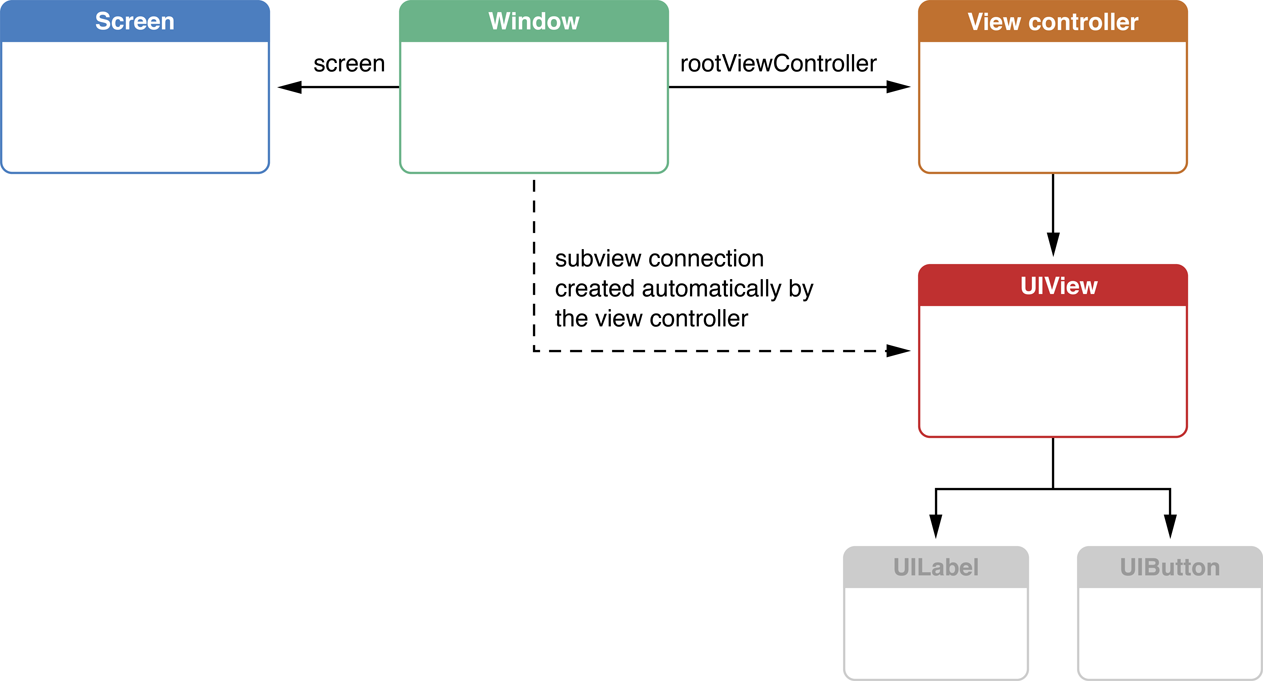
\includegraphics[width=.75\textwidth]{figuras/apple_window_view_controller_screen.png}
  \caption{Esquema relacionando os elementos da UI}
  \label{fig:relacionamento_UI}
\end{figure}

A figura \ref{fig:relacionamento_UI} representa as ligações entre os elementos de interface no iOS. A \texttt{\textbf{UIWindow}} aponta para a \texttt{\textbf{UIScreen}}, que representa a tela e seus limites, e aponta para  \texttt{\textbf{UIViewController}} inicial do aplicativo, que recebe o nome especial de \texttt{\textbf{RootViewController}}. A \texttt{\textbf{UIView}}, que representa os elementos gráficos da tela, e é controlada pela \texttt{\textbf{UIViewController}} inicial, é então adicionada à \texttt{\textbf{UIWindow}}, e assim temos a referência à controladora inicial e sua tela. Veremos a seguir a relação entre uma \texttt{\textbf{UIViewController}} e uma \texttt{\textbf{UIView}} com mais detalhes a seguir.

\subsection{UIView x UIViewController}


Um objeto do tipo \texttt{\textbf{UIView}}, ou apenas \emph{View}, é onde colocamos de fato os elementos visuais. Ela representa uma determinada área que pode conter objetos como \texttt{\textbf{UIButton}}, \texttt{\textbf{UILabel}} e \texttt{\textbf{UITextField}}, além de outras \emph{Views} inseridas, formando uma hierarquia de objetos que vão se orientar diretamente pelo posicionamento e comportamento da \texttt{\textbf{UIView}} maior.

A grande ideia a ser entendida e que diferencia uma \emph{View} de uma \emph{View Controller} é que um objeto de \texttt{\textbf{UIView}} contém estritamente elementos gráficos, sem nenhuma lógica do comportamento. Um objeto de \texttt{\textbf{UIView}} não entende e não deve entender as consequências de suas ações. Um \texttt{\textbf{UIButton}}, por exemplo, sabe como reagir quando é acionado mas não sabe qual tipo de ação ou mensagem foi gerada e nem pra onde ela foi enviada a partir do seu toque. Essa reação pode ser chamar um alerta, uma nova tela, uma animação, ou um acesso a \emph{web service}, mas o que acionou a ação não é responsabilidade do componente.

\begin{framed}

\textbf{Dica}: Deixando algumas coisas claras, uma tela pode conter uma só \emph{View} tomando todo o espaço ou várias \emph{Views} se dividindo, sendo elas totalmente independentes ou aninhadas. Além disso, você pode criar novas classes herdando de \texttt{\textbf{UIView}} para serem estanciadas dentro de uma \texttt{\textbf{UIViewController}}.
\end{framed}


Uma \emph{View Controller} é o que gerencia a lógica e comportamento de um conjunto específico de uma ou mais \emph{Views}, e é responsável por carregar e interagir com as \emph{Views} no momento certo e da forma correta. Um \texttt{\textbf{UIButton}} acionado envia um sinal para a \emph{View Controller}, que tem o papel de entender qual deve ser a resposta para esse evento, que pode ser algo como envio de dados, interação com as \emph{Views}, ou criação de animações.

Uma \emph{View Controller} é criada com uma única \emph{View} atrelada, e dentro dela podemos inserir mais elementos visuais, como até mais mais \emph{Views}.

\begin{figure}[H]
  \centering
  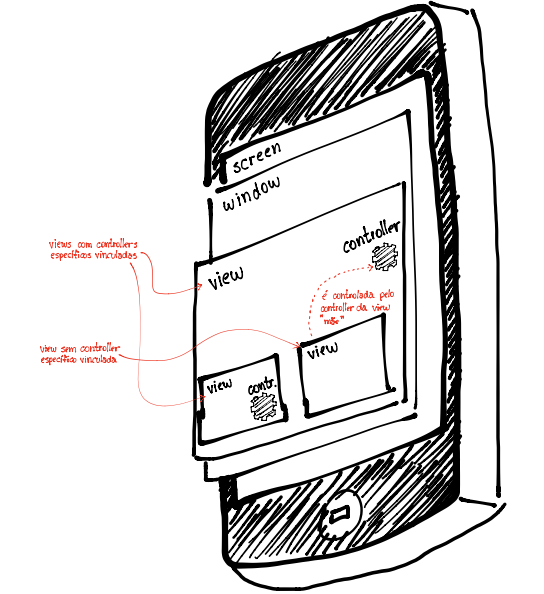
\includegraphics[width=.75\textwidth]{figuras/screen_hierarchy.png}
  \caption{Hierarquia dos componentes da tela}
  \label{fig:a}
\end{figure}


Sabendo que é possível criar uma classe para uma \emph{View} genérica, sem possuir uma \emph{View Controller} atrelada, como sabemos se criamos uma classe herdando de \texttt{\textbf{UIView}} ou de \texttt{\textbf{UIView Controller}}? Essa pergunta pode causar confusão no início, mas fica mais claro após entender exatamente o papel de cada uma.

Primeiramente seguimos a regra de que para cada tela completa criamos uma \emph{View Controller} para gerenciá-la, e nessa classe podemos inserir todos os elementos da tela. Porém há os casos em que a ideia é criar uma \emph{View} genérica a ser inserida no contexto de uma tela completa, \emph{View} essa que pode ser desde uma célula customizada para uma tabela até uma tabela completa, aí então devemos pensar se essa mesma \emph{View} terá algum comportamento ou se será unicamente visual. No caso de uma célula customizada, por exemplo, ela será apenas visual e assim deve ser uma simples classe de \texttt{\textbf{UIView}}; já no caso de uma tabela completa, ela vai precisar de um grande conjunto de lógica para o seu comportamento, portanto precisará de uma \emph{View Controller} própria, que no caso de tabelas tem uma classe especial chamada \texttt{\textbf{UITableViewController}}.

\subsection{Navegação entre telas}

\begin{figure}[h]
  \centering
  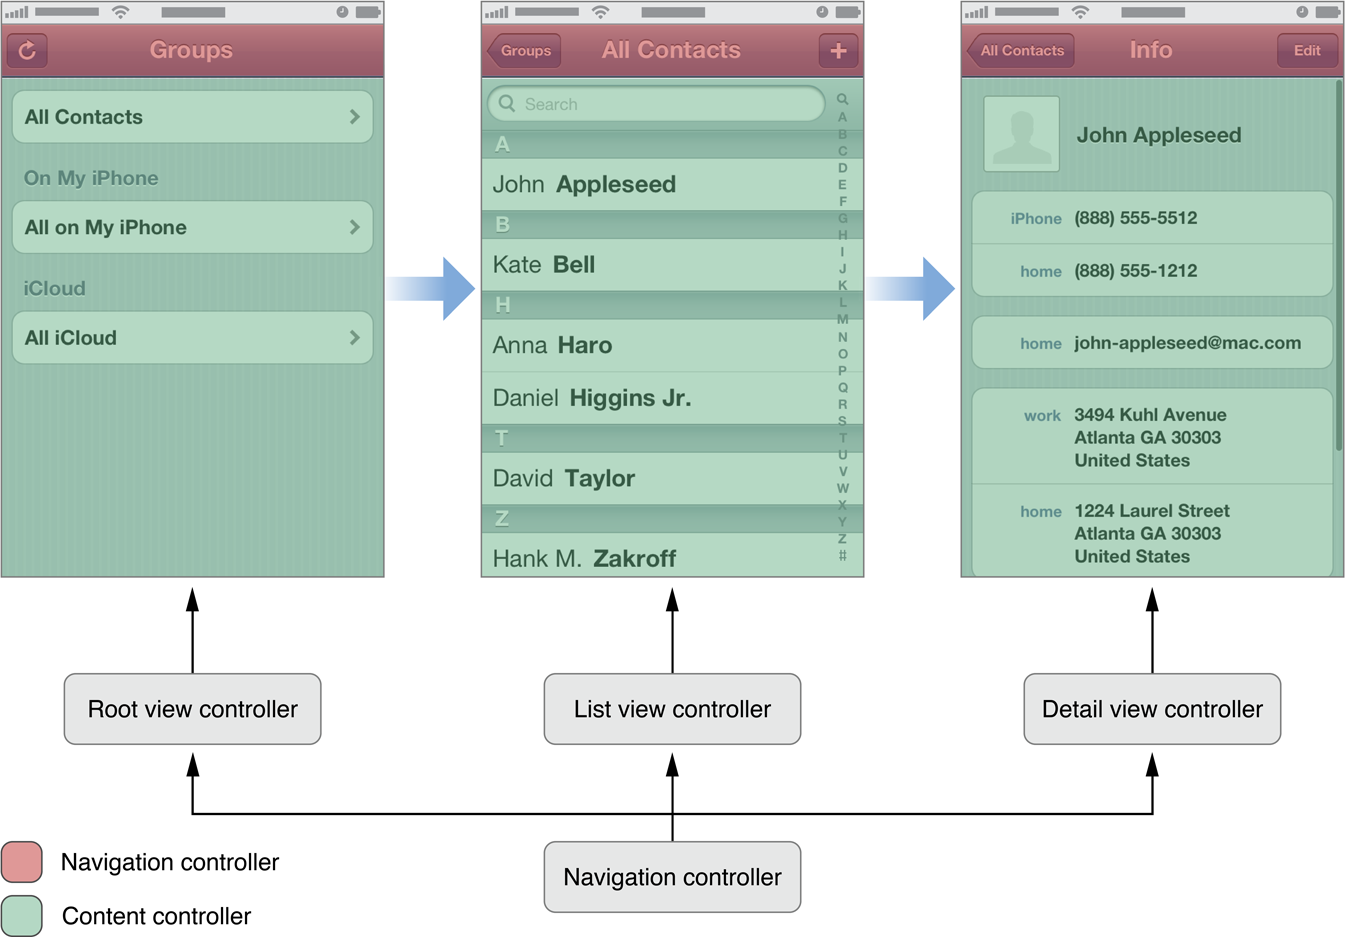
\includegraphics[width=\textwidth]{figuras/apple_navigation_interface.png}
  \caption{Funcionamento do Navigation Controller}
  \label{fig:a}
\end{figure}

Conforme vamos criando novas telas, precisamos de um modo de chamá-las e de retornar delas para a tela anterior. O iOS permite mais de um tipo de gerenciamento de navegação das telas, mas na maioria dos casos faremos uso do \emph{Navigation Controller}.

O \emph{Navigation Controller} funciona como uma pilha de \emph{View Controllers} que tem início sempre na já citada \texttt{\textbf{RootNavigationController}}, que será a tela inicial do aplicativo. Nós definimos uma única vez pelo código qual será nossa \texttt{\textbf{RootNavigationController}}, após isso trabalharemos apenas com métodos de \emph{push} e \emph{pop} para carregar e descarregar as telas. Graficamente, o \emph{Navigation Controller} é a barra superior nas telas dos aplicativos e que contém um botão de retorno e outros botões auxiliares.

Há um outro tipo de navegação complementar chamado \emph{Tab Bar Controller}, que nada mais é que uma nova tela, que pode inclusive estar contida na pilha do \emph{Navigation Controller}, e que traz duas ou mais telas divididas por abas.

\begin{figure}[h]
  \centering
  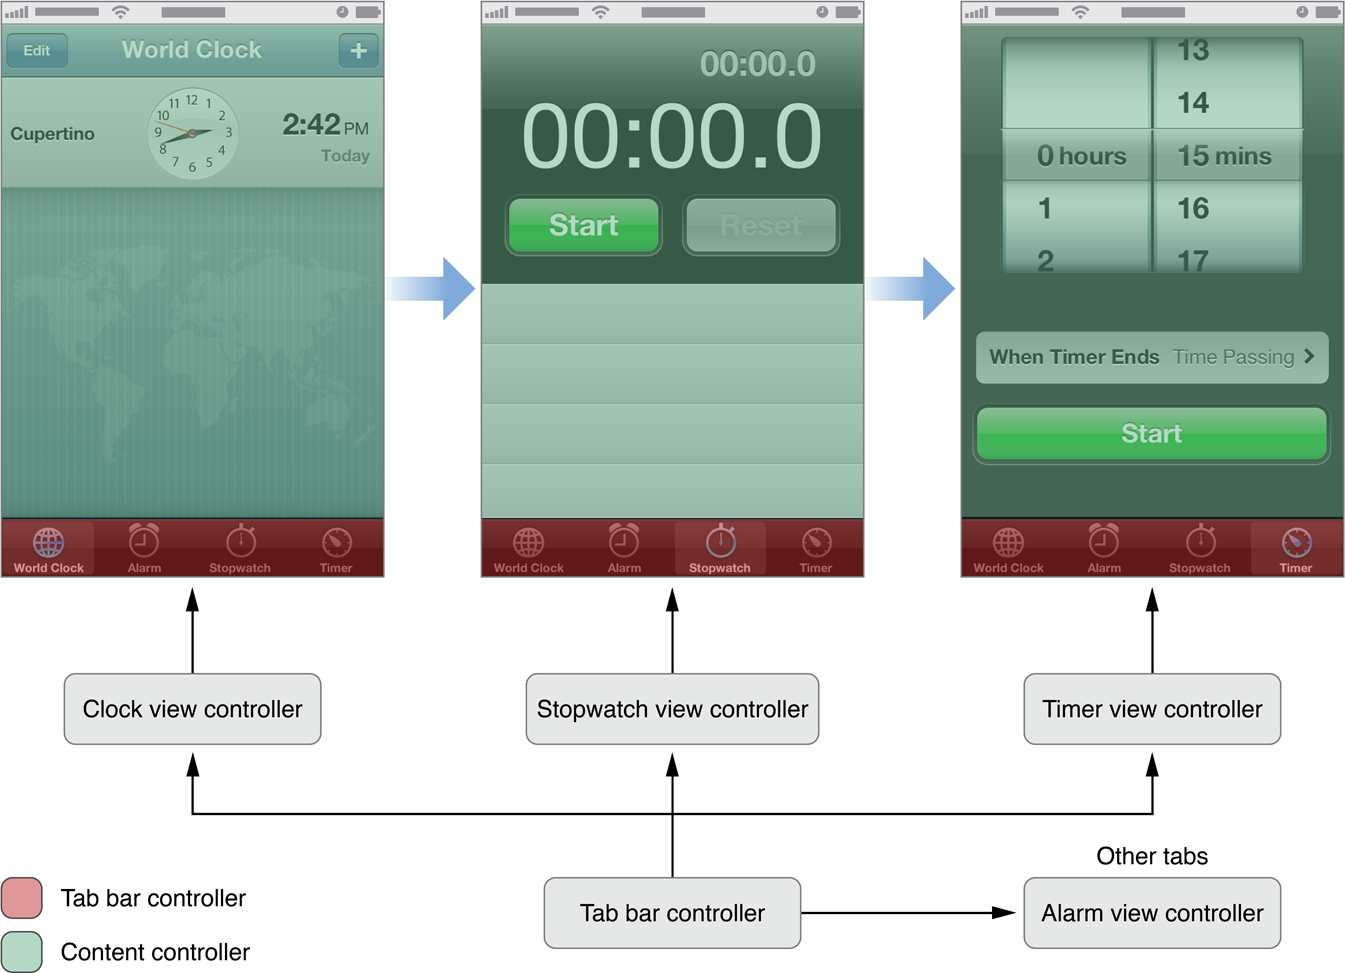
\includegraphics[width=\textwidth]{figuras/apple_tabbar_interface.png}
  \caption{Esquema do funcionamento do Tab Bar Controller}
  \label{fig:tab_bar_controller}
\end{figure}


Esta imagem é um modelo do funcionamento de uma \emph{Tab Bar Controller}. Diferente da \emph{Navigation Controller}, que funciona como uma pilha de telas, a \emph{Tab Bar Controller} aponta para todas as telas diretamente, e disponibiliza a escolha das telas astravés das abas. Na figura \ref{fig:tab_bar_controller} vemos a distinção do que consiste cada elemento graficamente.

\section{Interface Builder}

Para nos auxiliar na construção das telas, utilizeremos o \emph{Interface Builder} do XCode. Na criação de uma nova \emph{View Controller}, é criado um arquivo .xib atrelado a essa classe, que ligará automaticamente os objetos criados na interface ao código da classe.

O \emph{Interface Builder} é uma ferramenta muito poderosa e o utilizaremos principalmente para definir o posicionamento dos objetos, como as \emph{Views} e seus componentes, e para fazer a ligação dos \texttt{\textbf{IBOutlets}} e \texttt{\textbf{IBActions}} ao código.

\begin{framed}

\textbf{Dica}:  Lembrando que sempre podemos determinar o layout e a criação dos objetos diretamente no código, sendo o Interface Builder apenas um facilitador. Em diversos casos lidar com o código acaba sendo a melhor opção.
\end{framed}

\subsection{IBOutlets e IBActions}

\texttt{\textbf{IBOutlets}} representam uma ligação entre um objeto criado na interface pelo Interface Builder, como um botão ou um texto, e uma instância criada no código. Funciona como um ponteiro de um objeto do código para a sua representação gráfica, e assim podemos nos referenciar a esse elemento no código do \emph{View Controller} para definirmos seu comportamento e possíveis mudanças nas suas características.

Já uma \texttt{\textbf{IBAction}} representa uma mensagem enviada por um objeto da interface. A \texttt{\textbf{IBAction}} define o método que será chamado e que conterá o código com o comportamento desejado.

\section{Seu primeiro aplicativo}


Agora vamos enfim colocar a mão na massa e colocar em prática tudo que foi falado até agora. Abra o XCode e escolha a opção \emph{Create a new XCode project}.

\begin{figure}[H]
  \centering
  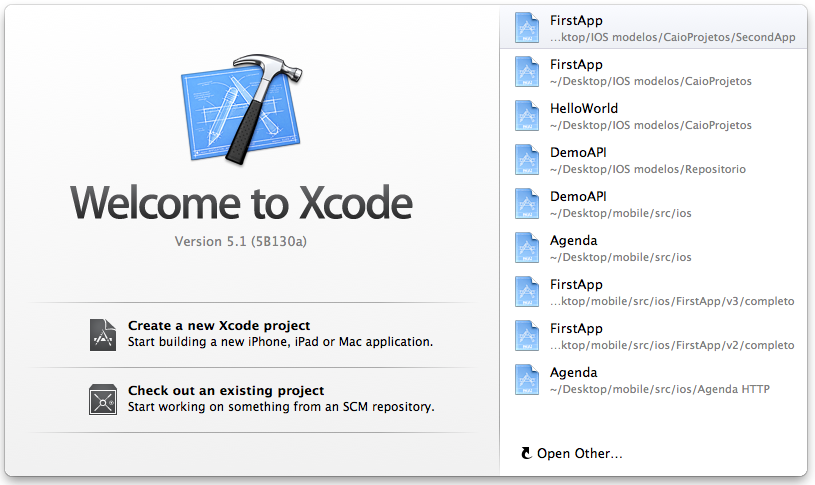
\includegraphics[width=.75\textwidth]{figuras/3/tela_boas_vindas_xcode.png}
  \caption{Tela de boas vindas do XCode}
  \label{fig:a}
\end{figure}

Na nova janela aberta, escolha a opção \emph{Empty Application} e em seguida \emph{Next}.

\begin{figure}[H]
  \centering
  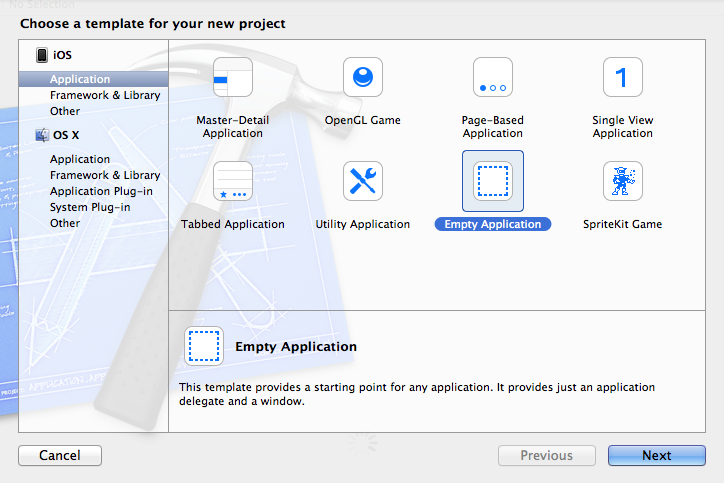
\includegraphics[width=.75\textwidth]{figuras/3/tela_novo_projeto_1.png}
  \caption{Criação de uma \emph{Empty Application}}
  \label{fig:a}
\end{figure}

Na próxima tela você pode escolher os detalhes do aplicativo. Os campos \emph{Product Name}, \emph{Organization Name} e \emph{Company Identifier} (nome do projeto, nome da organização e identificação da empresa, respectivamente) servem para escolhermos os detalhes do aplicativo, o campo \emph{Class Prefix} serve para que o XCode nomeie as classes iniciais com o prefixo indicado (caso deixe em branco será atribuido um nome padrão).

\begin{figure}[H]
  \centering
  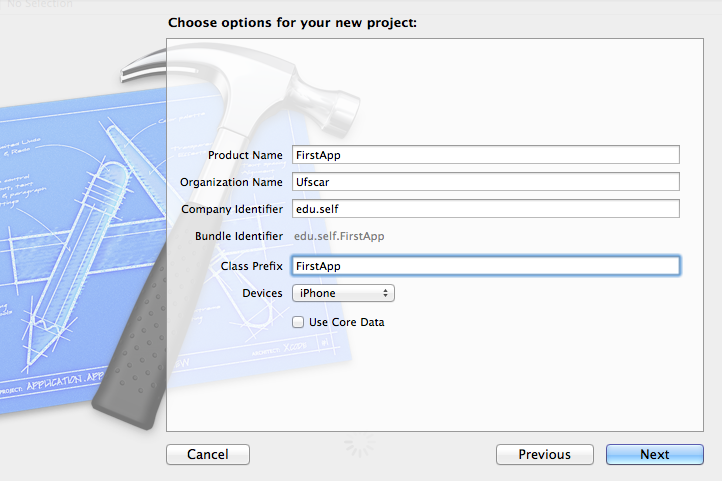
\includegraphics[width=.75\textwidth]{figuras/3/tela_novo_projeto_2.png}
  \caption{Opções para configuração do novo projeto}
  \label{fig:a}
\end{figure}

Deixe a opção \emph{Use Core Data} desmarcada, não iremos utilizar recursos referentes à armazenamento de dados nesse projeto.

\begin{framed}

\textbf{Dica}: Caso já tenha utilizado o XCode 4.6 ou anterior, irá notar que as opções 
\textit{ Use Automatic Reference Counting } e \textit{ Include Unit Tests } não estão presentes, isso porque já são definidas por padrão a partir do XCode 5.
\end{framed}

O XCode irá perguntar em qual lugar deve ser salvo o projeto, selecione uma pasta desejada e em seguida clique em \emph{Create} para concluir. 

\begin{figure}[H]
  \centering
  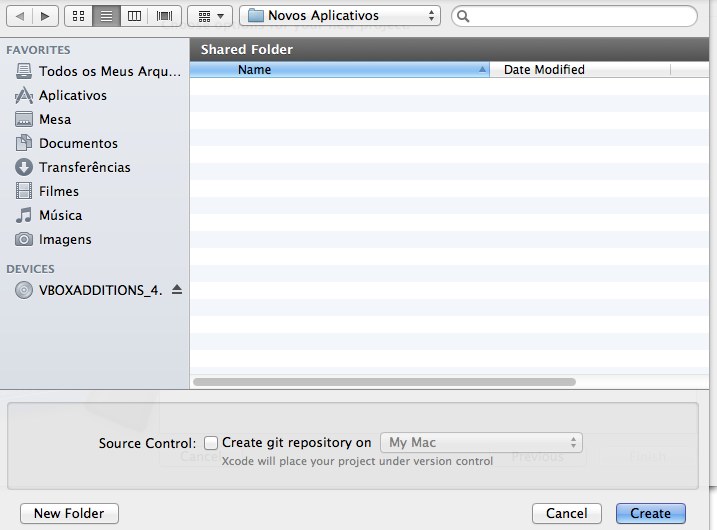
\includegraphics[width=.75\textwidth]{figuras/3/tela_novo_projeto_3.png}
  \caption{Finalizando a criação do novo projeto}
  \label{fig:a}
\end{figure}

XCode automaticamente cria o projeto "FirstApp" de acordo com as opções selecionadas.

\begin{figure}[H]
  \centering
  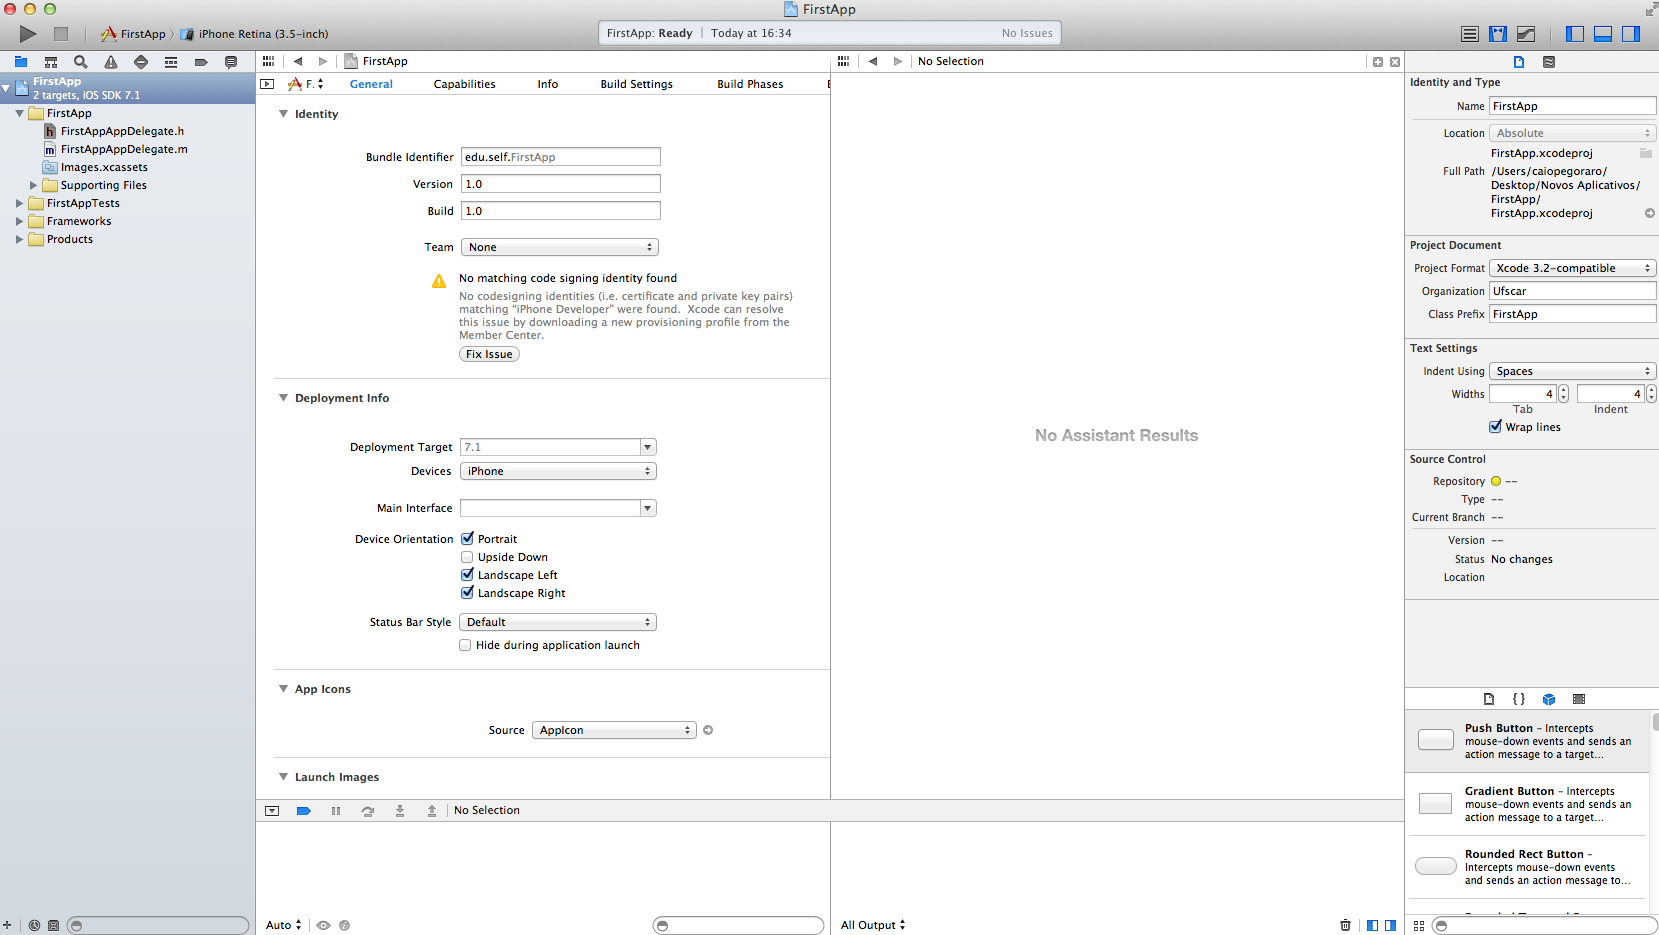
\includegraphics[width=.99\textwidth]{figuras/3/tela_novo_projeto_4.png}
  \caption{Tela principal do projeto}
  \label{fig:a}
\end{figure}

\begin{framed}

\textbf{Dica}: Para melhor visualizar os arquivos do projeto, use os ícones do canto superior direito para alterar a exibição dos códigos.
\end{framed}

\begin{figure}[H]
  \centering
  
\includegraphics[scale=1]{figuras/3/tela_opcao_exibicao.png}
  \caption{Opções para exibição do código na tela}
  \label{fig:a}
\end{figure}

\subsection{Primeira tela}


Primeiramente, vamos dar uma pequena olhada no ambiente do XCode. Na esquerda temos o \emph{Project Navigator}, podemos achar todos os arquivos do projeto nessa área. A parte central é a \emph{Editor Area}, faremos todas as edições (propriedades do projeto, códigos, interface, etc.) nessa área. Na área de baixo temos o \emph{Debug Area}, é exibida quando o aplicativo está sendo compilado. Na área da direita temos a \emph{Utility Area}, nela temos as propriedades dos arquivos e na parte inferior a lista de componentes para serem utilizados no projeto.

\begin{figure}[H]
  \centering
  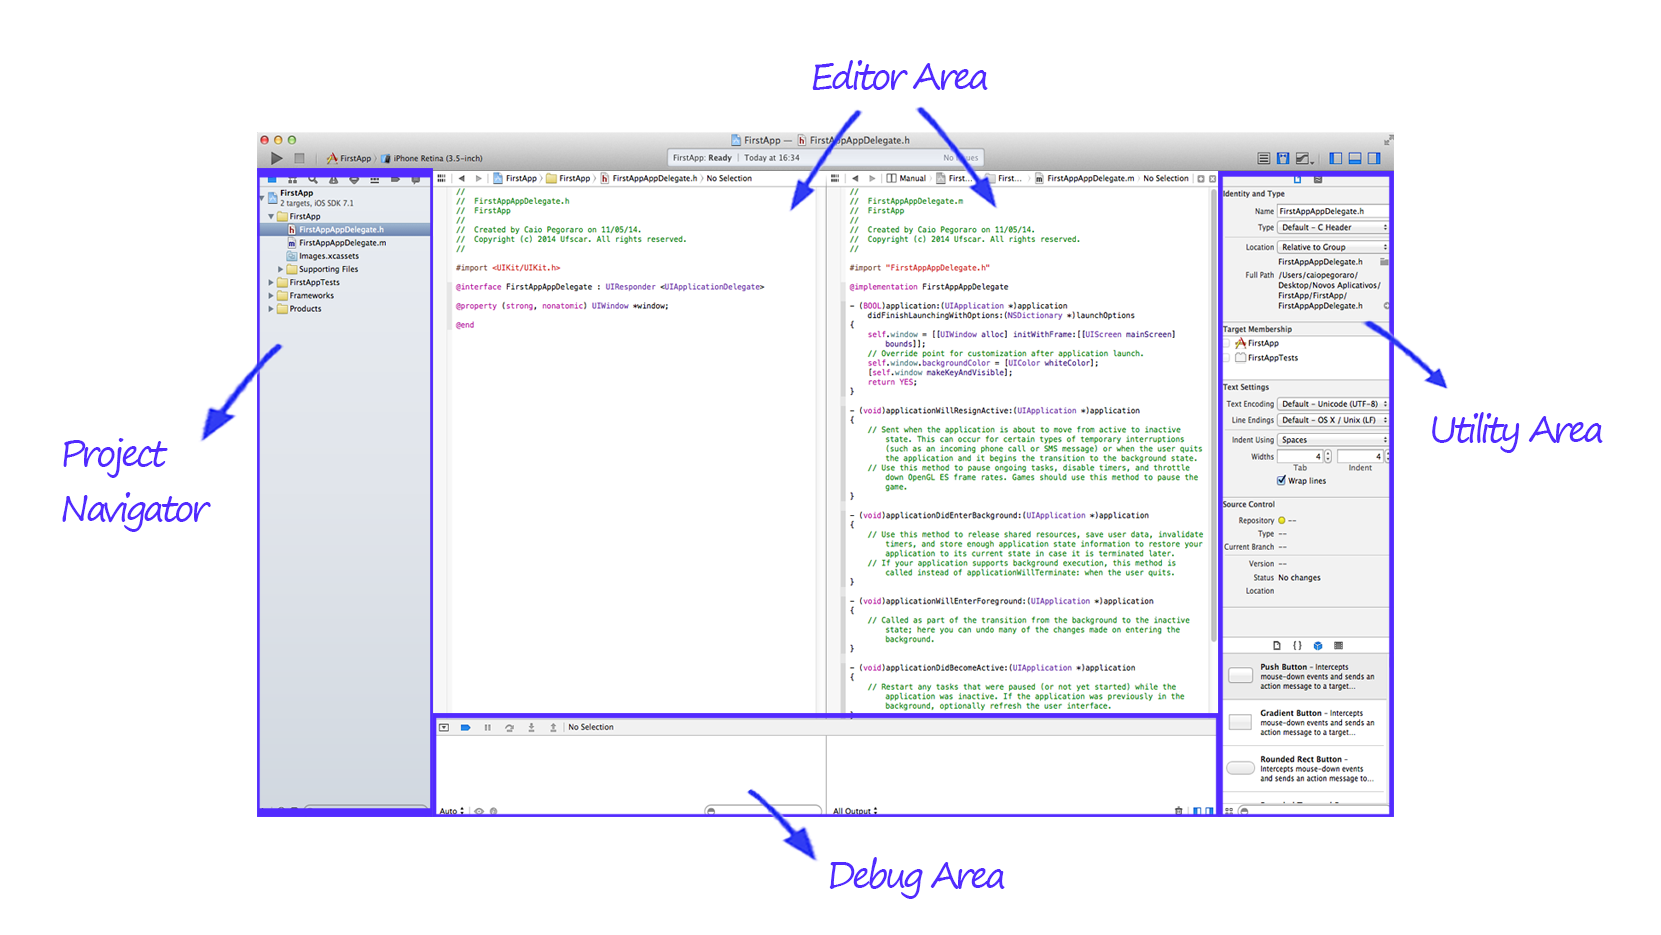
\includegraphics[width=.99\textwidth]{figuras/3/tela_principal_xcode.png}
  \caption{Organização do ambiente de desenvolvimento}
  \label{fig:a}
\end{figure}


Na parte superior temos mais algumas funções, podemos iniciar o aplicativo no simulador através do \emph{Run button}. Em \emph{Select iphone simulador} é possível alterar a versão do simulador para testarmos a aplicação em diversos modelos de dispositivos. O \emph{Editor buttons} altera a visualização dos códigos na tela, preferencialmente utilizaremos a tela dividida (opção central). Em \emph{View selections} é possível ativar ou desativar a exibição de segmentos da tela do XCode.

\begin{figure}[H]
  \centering
  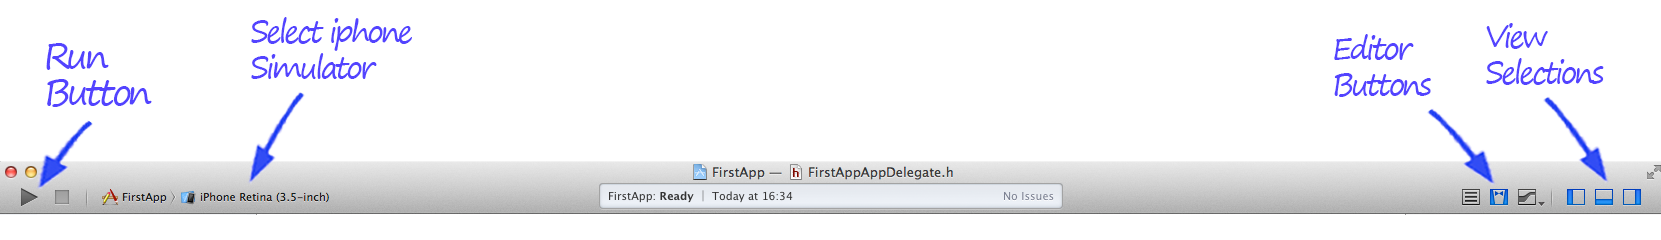
\includegraphics[width=.85\textwidth]{figuras/3/tela_principal_xcode_run.png}
  \caption{Estruturas de controle para o novo projeto}
  \label{fig:a}
\end{figure}

\begin{framed}

\textbf{Dica}: Caso o XCode não exiba nenhuma informação na
\textit{Utility Area}, tente clicar no projeto principal ou no arquivo desejado presente no \textit{Project Navigator}.
\end{framed}


 Selecione o arquivo \emph{FirstAppAppDelegate.h}. Na tela dividida vemos a classe principal (O arquivo .h e .m), será utilizada posteriormente para chamarmos a tela inicial do aplicativo.

\begin{figure}[H]
  \centering
  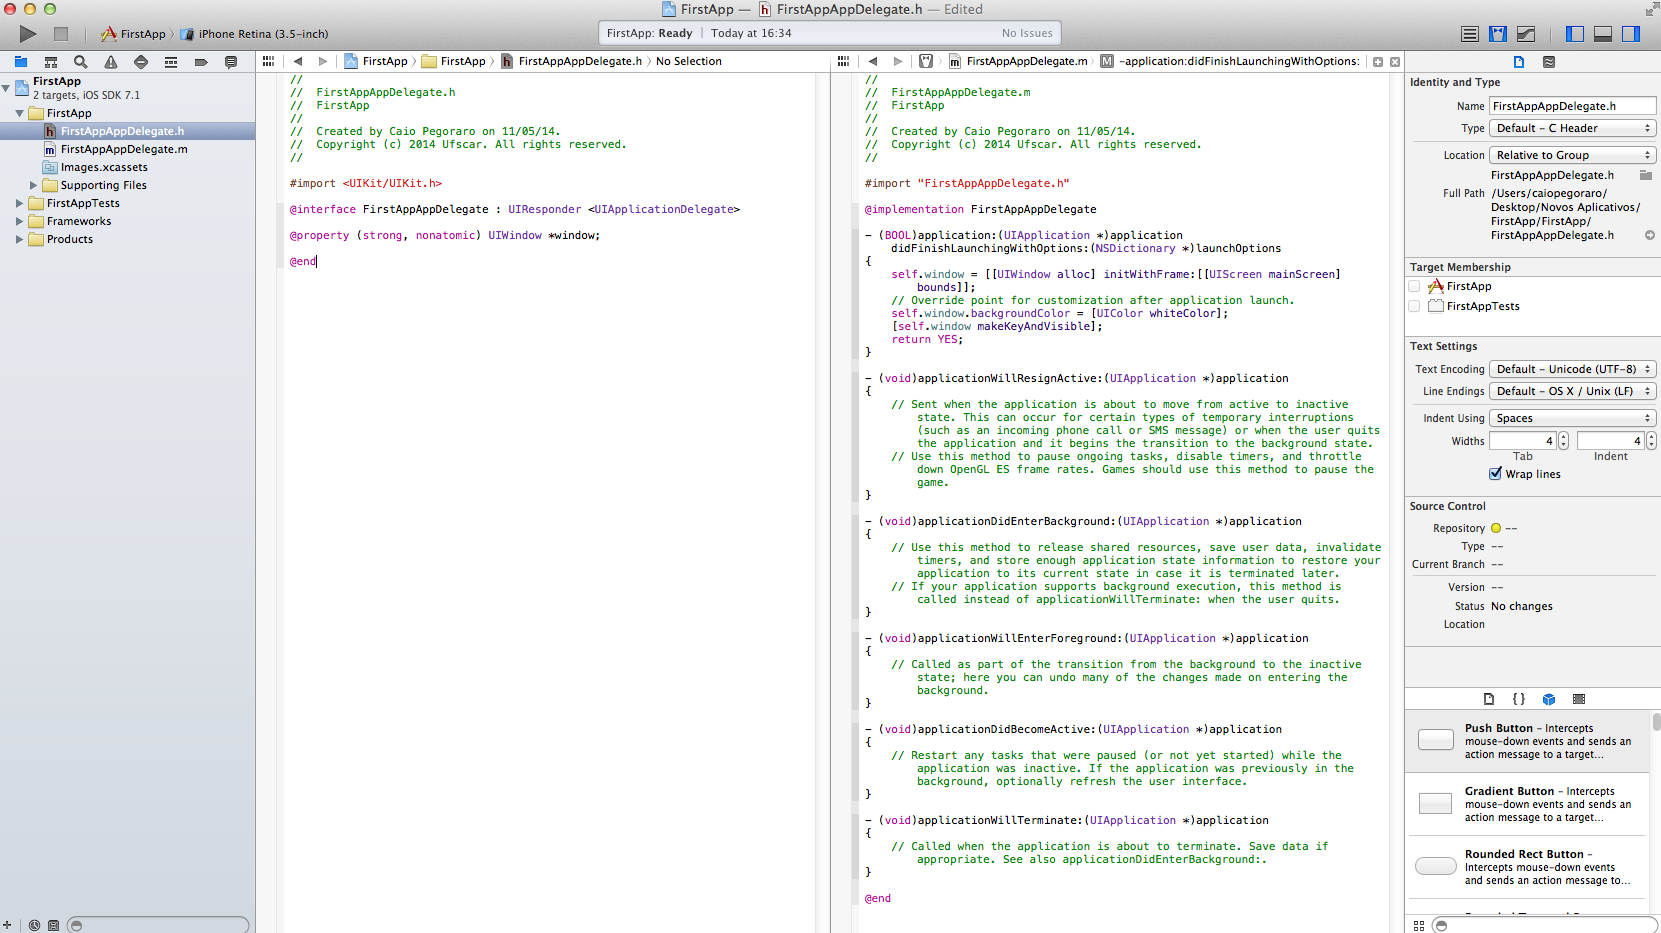
\includegraphics[width=.99\textwidth]{figuras/3/tela_novo_projeto_5.png}
  \caption{Classe principal do projeto}
  \label{fig:a}
\end{figure}


Para prosseguir precisamos criar uma tela inicial para o aplicativo, clique com o botão direito na pasta do projeto (pasta \emph{FirstApp} localizada no \emph{Project Navigator}) e em seguida na opção \emph{New File}.

\begin{figure}[H]
  \centering
  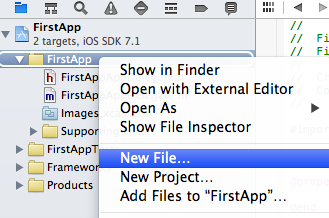
\includegraphics[width=.35\textwidth]{figuras/3/tela_novo_projeto_6.png}
  \caption{Adicionando um novo arquivo ao projeto}
  \label{fig:a}
\end{figure}


Selecione a opção \emph{Objective-C class} dentro da categoria \emph{Cocoa Touch}.

\begin{figure}[H]
  \centering
  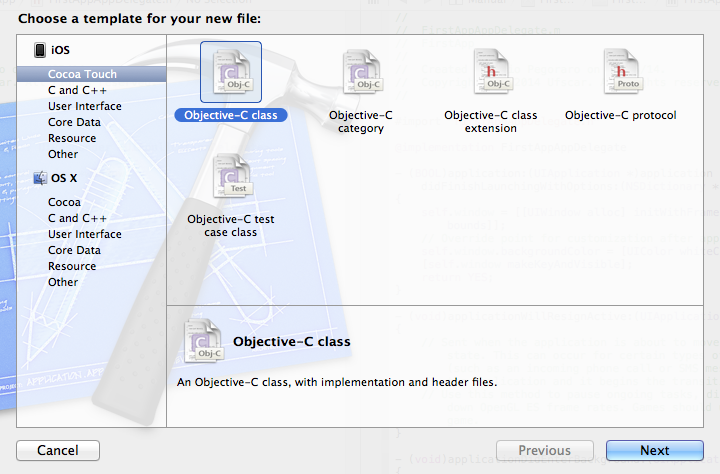
\includegraphics[width=.75\textwidth]{figuras/3/tela_novo_projeto_7.png}
  \caption{Adicionando uma nova interface ao projeto}
  \label{fig:a}
\end{figure}


Em \emph{Class} deixe com o nome padrão de \emph{FirstAppViewController} e em \emph{Subclass of} deixe como \texttt{\textbf{UIViewController}}. Marque a opção \emph{Also create XIB file} e clique em \emph{Next}.

\begin{figure}[H]
  \centering
  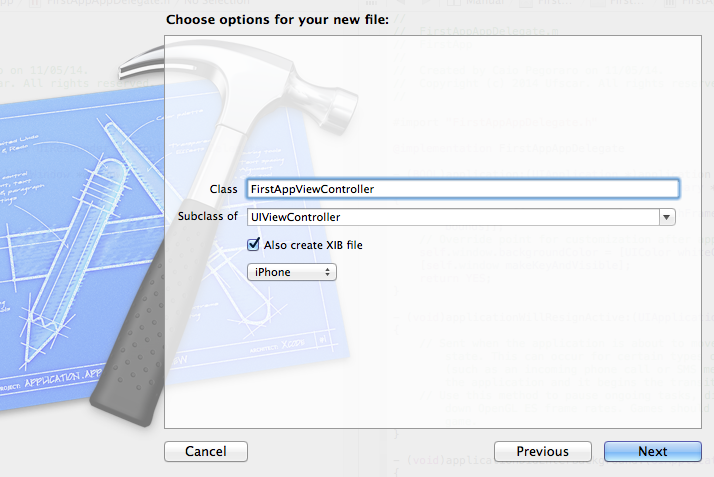
\includegraphics[width=.75\textwidth]{figuras/3/tela_novo_projeto_8.png}
  \caption{Configurando as opções para a nova interface}
  \label{fig:a}
\end{figure}


Na próxima tela clique em \emph{Create} para finalizar.

\begin{figure}[H]
  \centering
  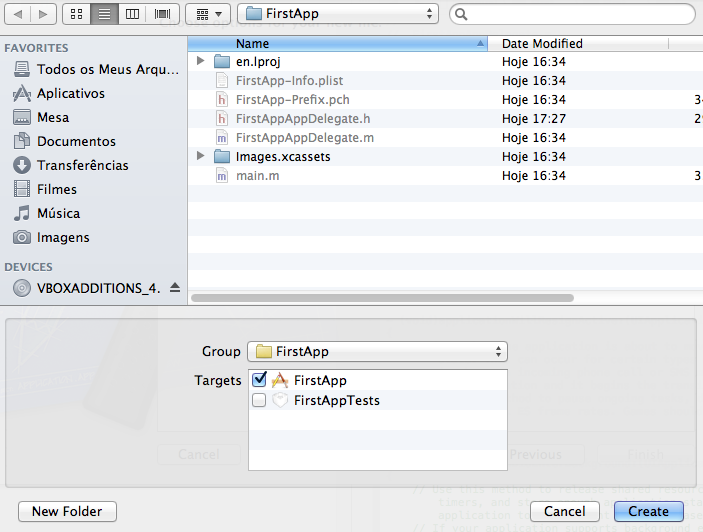
\includegraphics[width=.75\textwidth]{figuras/3/tela_novo_projeto_9.png}
  \caption{Finalizando a adição da nova interface ao projeto}
  \label{fig:a}
\end{figure}


Foram gerados 3 novos arquivos referentes à tela inicial do aplicativo: \emph{FirstAppViewController.h}, \emph{FirstAppViewController.m} e \emph{FirstAppViewController.xib}. Se selecionarmos o \emph{FirstAppViewController.xib} veremos uma tela em branco.

\begin{figure}[H]
  \centering
  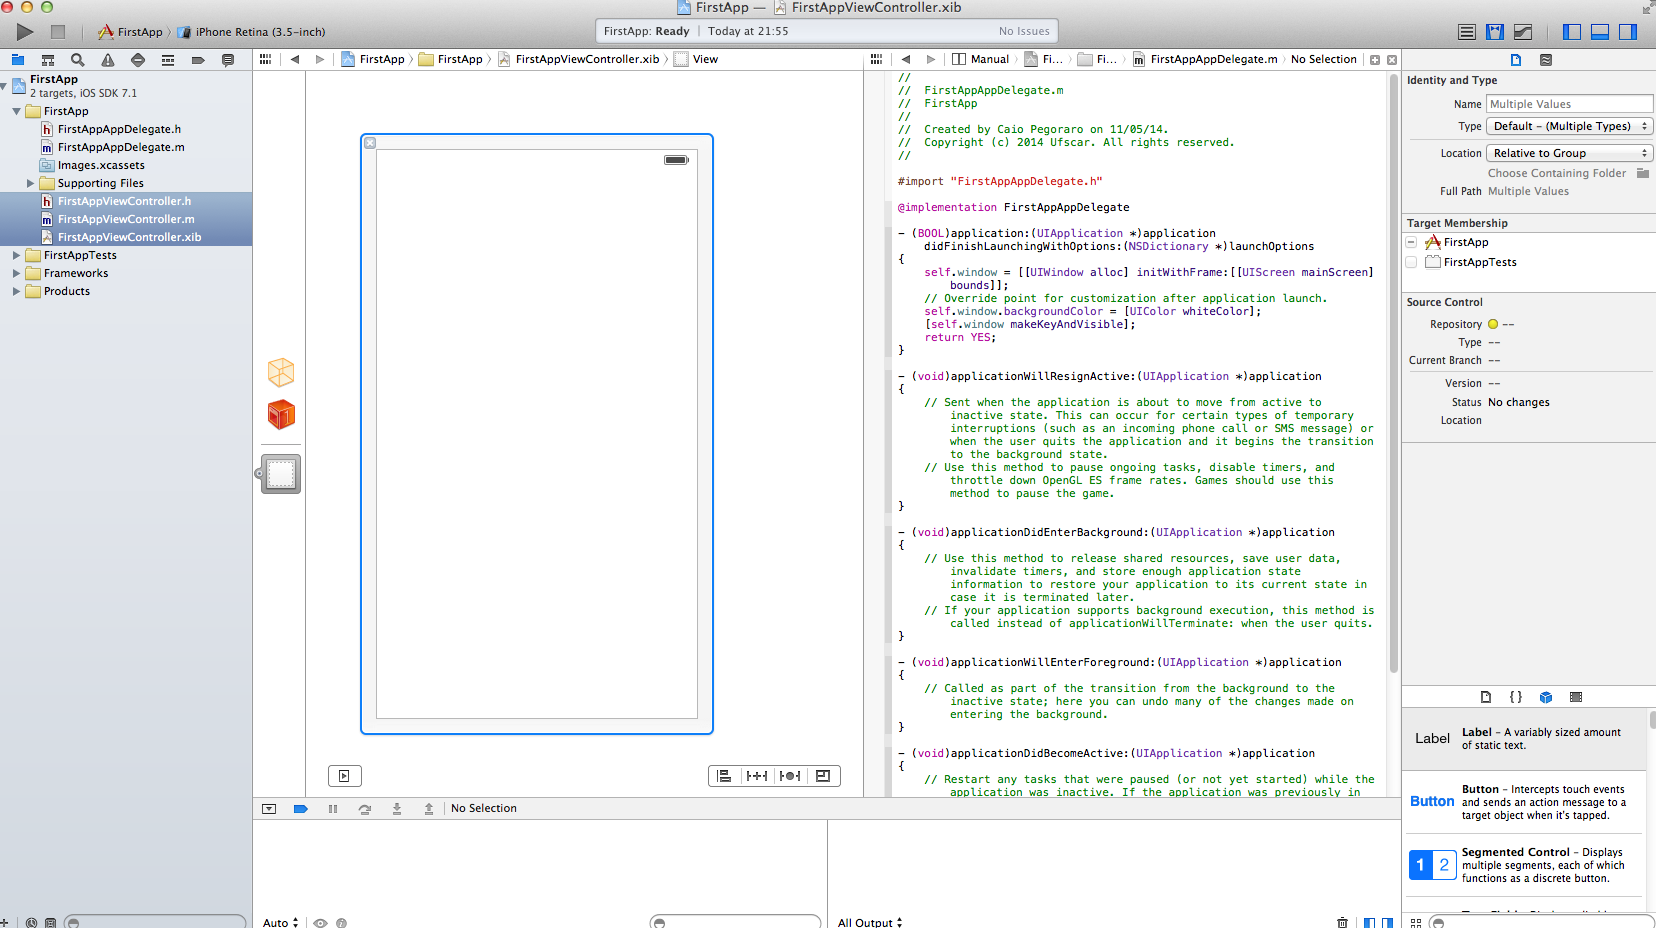
\includegraphics[width=.99\textwidth]{figuras/3/tela_novo_projeto_10.png}
  \caption{Interface builder no Xcode}
  \label{fig:a}
\end{figure}


Arquivos .xib são arquivos de construção de interface (Interface builder) que armazenam a interface do usuário do aplicativo. Ao clicar neles o XCode automaticamente exibirá a interface para que você possa edita-lá através do método \emph{drag-and-drop} (arrastar e soltar).
Os arquivos .h se referem aos arquivos de cabeçalho (header files) e os .m aos arquivos de implementação (implementation files).


No canto superior direito temos 3 conjuntos de ícones. No conjunto dos botões \emph{View Selections}, clique no ícone da direita para abrir a seção de opções do Interface Builder (a \emph{Utility Area}). Nessa parte poderemos ver e editar as características de qualquer objeto selecionado da tela, desde um botão a uma View, e alternar as opções entre as abas.

\begin{figure}[H]
  \centering
  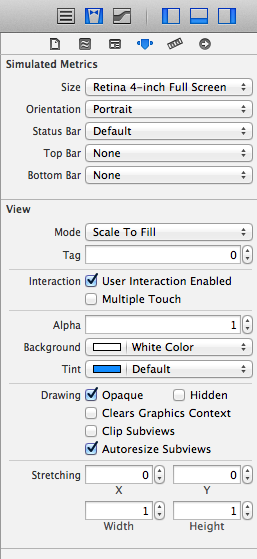
\includegraphics[scale=0.5]{figuras/3/tela_novo_projeto_11.png}
  \caption{Barra lateral de opções do Interface Builder}
  \label{fig:a}
\end{figure}


No canto inferior direito está presente a seção de \emph{Objetos}, os quais podem ser selecionados e arrastados para a interface do aplicativo.

\begin{figure}[H]
  \centering
  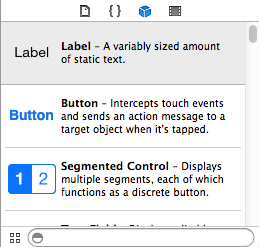
\includegraphics[scale=0.5]{figuras/3/tela_novo_projeto_12.png}
  \caption{Objetos disponíveis no Interface Builder}
  \label{fig:a}
\end{figure}

\begin{framed}

\textbf{Dica}: Para visualizar melhor os componentes, clique no ícone localizado no canto inferior esquerdo da seção de objetos.
\end{framed}

Outro item a ser configurado encontra-se na tela central do XCode, não é um item necessário mas irá facilitar os próximos passos do desenvolvimento. Verifique que ao lado esquerdo da tela central do aplicativo (\emph{Editor Area}) existem 2 blocos e uma caixa circulada de cinza, bem ao lado direito desses itens existe uma barra cinza claro vertical, clique nessa barra e arraste-a para a direita de forma a expandir essa área.

\begin{figure}[H]
  \centering
  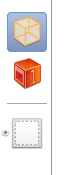
\includegraphics[scale=0.5]{figuras/3/tela_novo_projeto_14.png}
  \caption{Alterar modo de exibição do \emph{Placeholders}}
  \label{fig:a}
\end{figure}


O resultado final é uma exibição mais detalhada dos itens. Utilizaremos esse item mais tarde para fazer a ligação dos componentes da interface com os do código.

\begin{figure}[H]
  \centering
  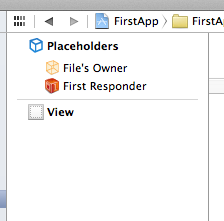
\includegraphics[scale=0.7]{figuras/3/tela_novo_projeto_15.png}
  \caption{Novo modo de exibição do \emph{Placeholders}}
  \label{fig:a}
\end{figure}



Vamos inicialmente adicionar um \texttt{\textbf{UILabel}} e um \texttt{\textbf{UIButton}} com textos de exemplo à tela. Arraste os objetos de forma a obter um layout parecido com o mostrado na figura \ref{fig:arrastando_itens}.

\begin{figure}[H]
  \centering
  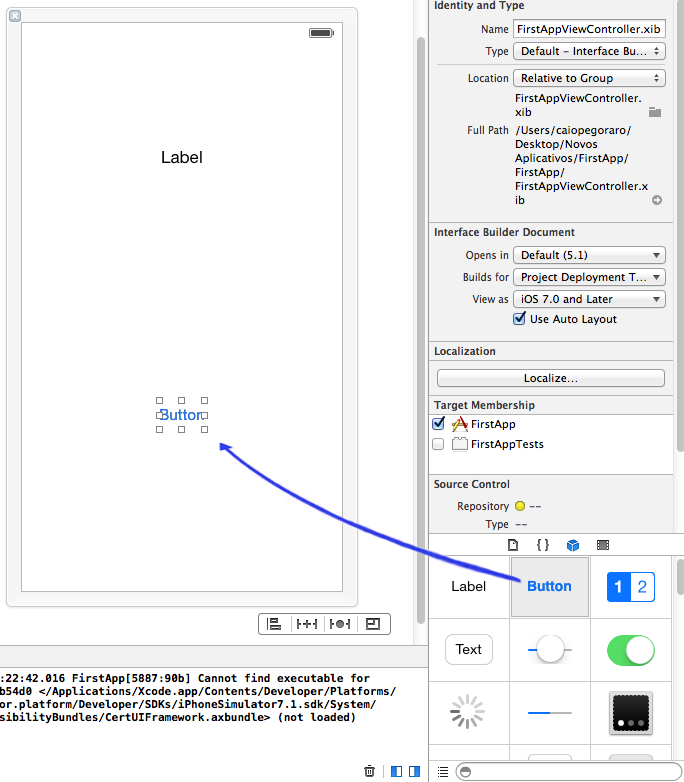
\includegraphics[width=.75\textwidth]{figuras/3/tela_novo_projeto_19.png}
  \caption{Arrastando componentes para interface do aplicativo}
  \label{fig:arrastando_itens}
\end{figure}

\begin{figure}[H]
  \centering
  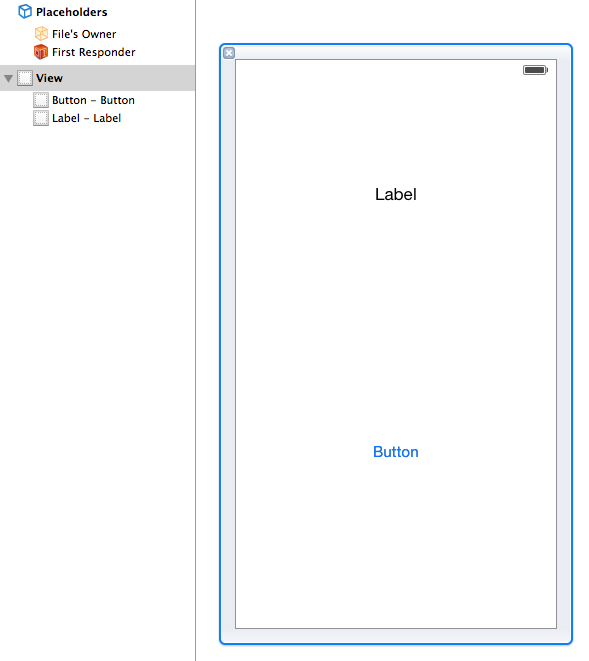
\includegraphics[width=.75\textwidth]{figuras/3/tela_novo_projeto_16.png}
  \caption{Interface com os primeiros objetos criados}
  \label{fig:a}
\end{figure}

Se tentar rodar o aplicativo agora, será exibida uma tela em branco. Isso porque o aplicativo não foi configurado para carregar a nova tela criada. É necessário inserir a importação da classe da interface no arquivo \emph{FirstAppAppDelegate.h}.

\begin{listing}[H]
\begin{minted}[linenos=true,frame=lines,framesep=2mm,tabsize=2,numbersep=5pt]{objective-c}
#import "FirstAppViewController.h"
\end{minted}
\caption{Importando a classe da interface inicial}
\end{listing}


Selecionando o \emph{FirstAppAppDelegate.m} temos o método \emph{didFinishLaunchingWithOptions}, adicione o seguinte código logo após \emph{self.window.backgroundColor = [UIColor whiteColor];}:

\begin{listing}[H]
\begin{minted}[linenos=true,frame=lines,framesep=2mm,tabsize=2,numbersep=5pt]{objective-c}
FirstAppViewController *viewController =[[FirstAppViewController alloc] 
		initWithNibName:@"FirstAppViewController" bundle:nil];
		
self.window.rootViewController = viewController;    
\end{minted}
\caption{Configurando a tela inicial do aplicativo}
\end{listing}


Cria-se, na linha 1, um objeto do tipo \texttt{\textbf{FirstAppViewController}} e na linha 4 definimos como a tela principal que será carregada quando o aplicativo for inicializado. 

Nesse momento, executando o aplicativo através do \emph{Run Button} será exibida a tela do \emph{FirstAppViewController} e não mais uma tela em branco.

\begin{figure}[H]
  \centering
  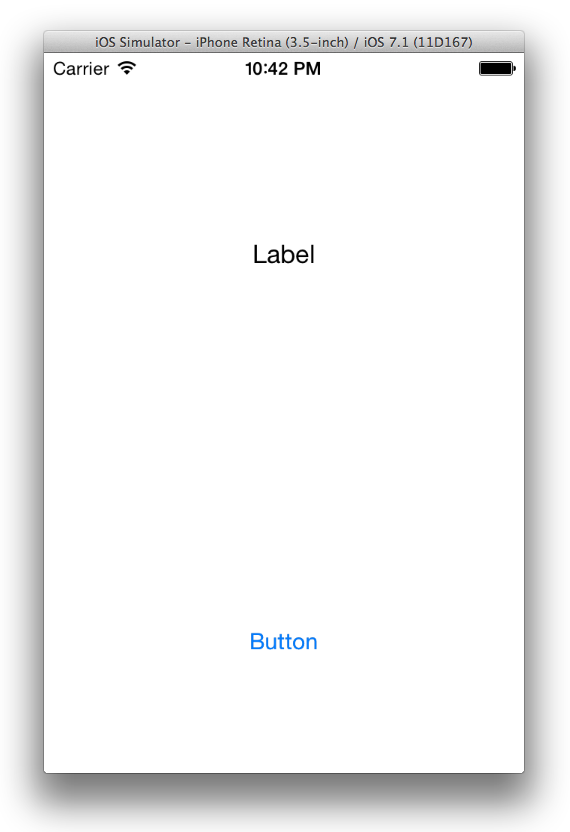
\includegraphics[width=.55\textwidth]{figuras/3/tela_novo_projeto_18.png}
  \caption{Exibindo tela inicial do aplicativo no simulador}
  \label{fig:a}
\end{figure}

\begin{framed}

\textbf{Dica}: Os simuladores do iOS 6.0 e 6.1 apresentam o visual de um iphone, essa característica não está presente nas versões 7.0 e 7.1 (apesar de ainda ser possível alterar o tamanho da tela do simulador pressionando a tecla \textit{Comando} e as teclas 1, 2 ou 3). Para utilizar o simulador da versão 6 é necessário instalar o componente referente a essa versão, alterar o \textit{Deployment Target} localizado nas propriedades do projeto (clicando no ícone do projeto no \textit{Project Navigator}) e por fim alterar o dispositivo do simulador para um que utilize o iOS 6.\end{framed}


Clicando 2 vezes no \emph{button} é possível editar o texto que está sendo exibido, colocaremos como sendo \emph{Primeiro Botão}.

\begin{figure}[H]
  \centering
  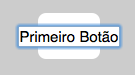
\includegraphics[scale=0.7]{figuras/3/tela_novo_projeto_20.png}
  \caption{Editando o texto do botão criado}
  \label{fig:a}
\end{figure}

\begin{framed}

\textbf{Dica}: Caso esteja utilizando o MAC OS X em um computador com um teclado padrão Windows, a tecla \textit{Windows }é equivalente a tecla \textit{Comando}.
\end{framed}

Para que o botão execute uma ação, é necessário criar uma \texttt{\textbf{IBAction}}. Selecione o arquivo \emph{FirstAppViewController.h} para adicionar o seguinte trecho de código:

\begin{listing}
\begin{minted}[linenos=true,frame=lines,framesep=2mm,tabsize=2,numbersep=5pt]{objective-c}
-(IBAction)mostrarMsg;
\end{minted}
\caption{Adicionando uma \texttt{\textbf{IBAction}} para exibir uma mensagem na tela}
\end{listing}

Em seguida, selecione o arquivo \emph{FirstAppViewController.m} para adicionar o  trecho de código a seguir:

\begin{listing}
\begin{minted}[linenos=true,frame=lines,framesep=2mm,tabsize=2,numbersep=5pt]{objective-c}
-(IBAction)mostrarMsg {
    UIAlertView *AlertaOlaMundo = [[UIAlertView alloc] 
    	initWithTitle:@"Meu primeiro app" message:@"Ola mundo!" 
	delegate:nil cancelButtonTitle:@"Fechar" otherButtonTitles:nil];
    
	[AlertaOlaMundo show];
}
\end{minted}
\caption{Adicionando uma \emph{IBAction}}
\end{listing}


O código cria um objeto do tipo \texttt{\textbf{UIAlertView}} na linha 2, já inicializando-o com alguns textos para exibição. Na linha 6 é invocado um método da classe para que o alerta seja exibido na tela. 

Agora clicando novamente no arquivo \emph{FirstAppViewController.xib} localizado na \emph{Project Navigator}, vemos a tela com a \emph{label} e o \emph{button} criados anteriormente. O botão não realiza nenhuma ação no momento, nesse caso deseja-se que ele execute a \texttt{\textbf{IBAction}} \emph{mostraMsg}, para ligar o botão à essa ação basta segurar a tecla \emph{Control}, clicar no objeto \emph{button} da tela e mover o mouse sobre o \emph{File's Owner}.

\begin{framed}

\textbf{Dica}: A tecla \textit{Control} é equivalente à tecla textit{Ctrl} esquerda em outros formatos de teclado.
\end{framed}

\begin{figure}[H]
  \centering
  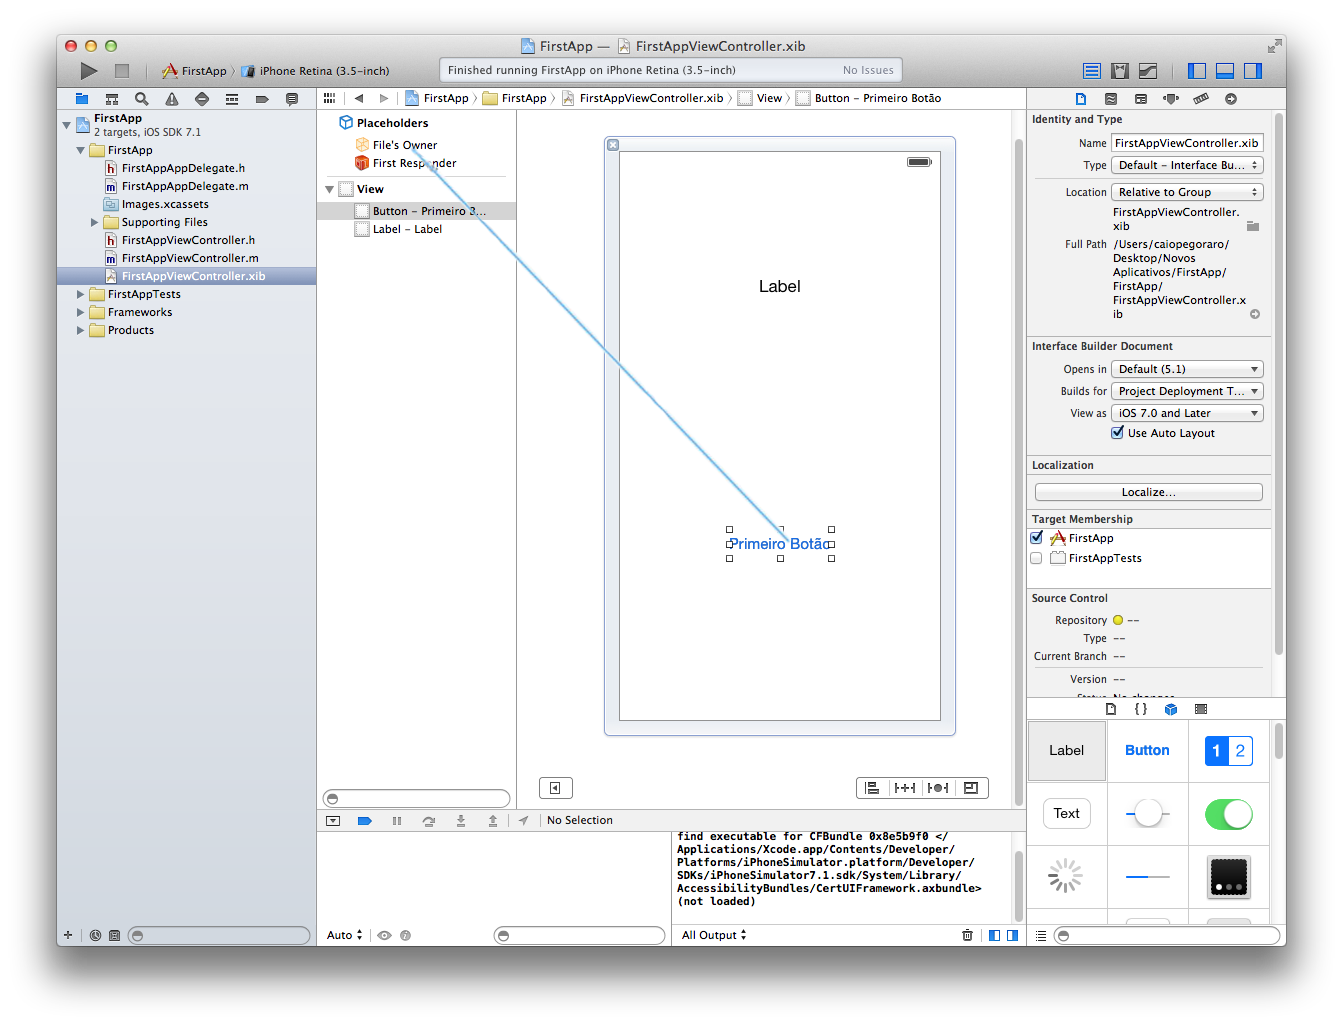
\includegraphics[width=0.7\textwidth]{figuras/3/tela_novo_projeto_23.png}
  \caption{Conectando o \emph{button} com a \texttt{\textbf{IBAction}}}
  \label{fig:a}
\end{figure}

Ao soltar o click será exibida a opção para conectar o botão à \texttt{\textbf{IBAction}}, basta clicar na opção \emph{mostrarMsg} para concluir.

\begin{figure}[H]
  \centering
  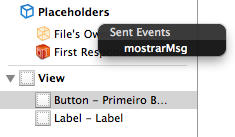
\includegraphics[scale=1]{figuras/3/tela_novo_projeto_24.png}
  \caption{Finalizando a conexão do \emph{button} com a \texttt{\textbf{IBAction}}}
  \label{fig:a}
\end{figure}

Há outra forma de conectar uma \texttt{\textbf{IBAction}} à um botão (também vale para outros tipos), basta clicar em \texttt{\textbf{File's Owner}} e arrastar a opção desejada dentre as listadas no lado direito da interface do XCode até o componente.

\begin{figure}[H]
  \centering
  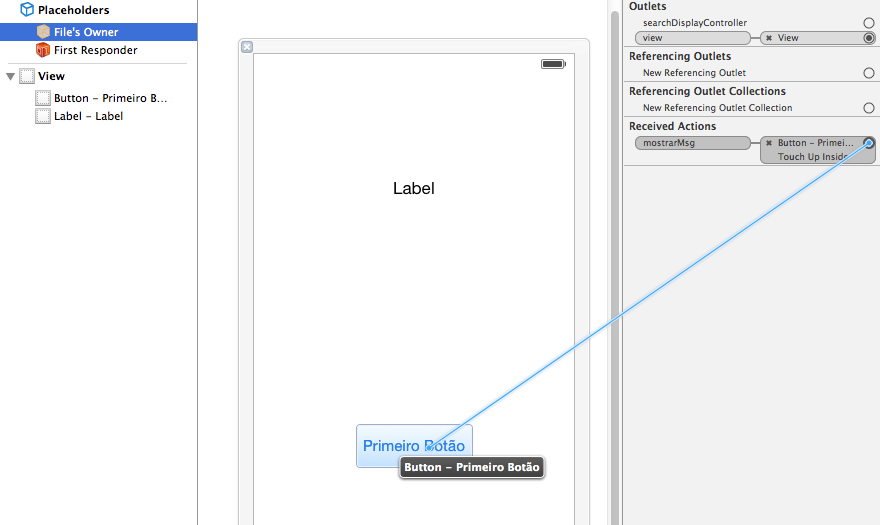
\includegraphics[width=0.7\textwidth]{figuras/3/tela_novo_projeto_52.png}
  \caption{Maneira alternativa para conectar o \emph{button} com a \texttt{\textbf{IBAction}}}
  \label{fig:a}
\end{figure}

Clicando no \emph{Run Button} o projeto será iniciado no simulador e o botão, ao ser clicado, exibirá uma mensagem na tela.

\begin{figure}[H]
  \centering
  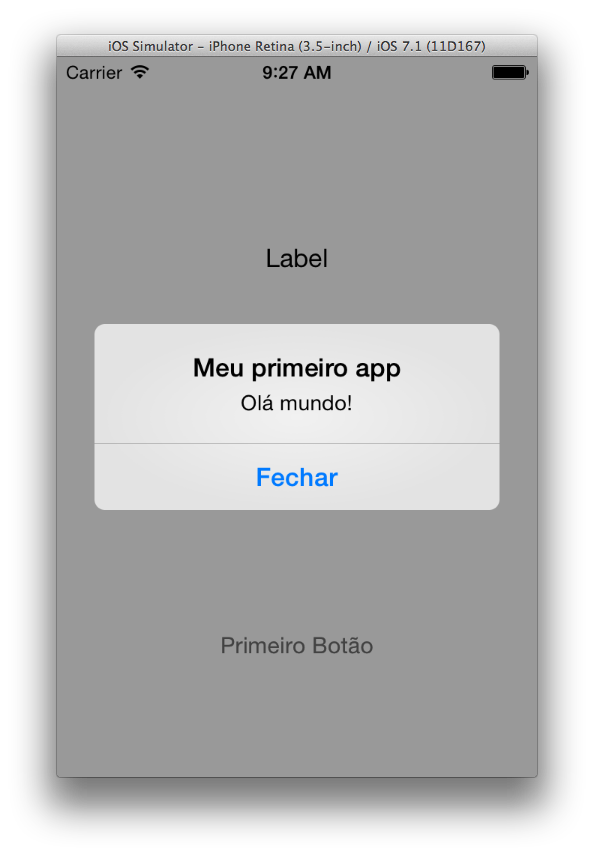
\includegraphics[width=.55\textwidth]{figuras/3/tela_novo_projeto_25.png}
  \caption{Exibindo a mensagem na tela do aplicativo}
  \label{fig:a}
\end{figure}


Agora precisamos definir o funcionamento da \emph{Navigation Controller}, responsável pela navegação entre as telas do aplicativo. Abra o arquivo \emph{FirstAppAppDelegate.h} e adicione a seguinte propriedade:

\begin{listing}
\begin{minted}[linenos=true,frame=lines,framesep=2mm,tabsize=2,numbersep=5pt]{objective-c}
@property (strong, nonatomic) UINavigationController
									   *navController;
\end{minted}
\caption{Definição da \emph{Navigation Controller}}
\end{listing}


Esta propriedade representa a \emph{Navigation Controller} em si. No arquivo \emph{FirstAppAppDelegate.m}, deixaremos o primeiro método deste jeito:

\begin{listing}[H]
\begin{minted}[linenos=true,frame=lines,framesep=2mm,tabsize=2,numbersep=5pt]{objective-c}
- (BOOL)application:(UIApplication *)application 
	didFinishLaunchingWithOptions:(NSDictionary *)launchOptions{
    self.window = [[UIWindow alloc] 
    		initWithFrame:[[UIScreen mainScreen] bounds]];

    self.window.backgroundColor = [UIColor whiteColor];
    
    self.window = [[UIWindow alloc] 
    		initWithFrame:[[UIScreen mainScreen] bounds]];
    
    FirstAppViewController *viewController =
    	[[FirstAppViewController alloc] 
    		initWithNibName:@"FirstAppViewController" bundle:nil];
    
    self.window.rootViewController = viewController;

    self.navController = [[UINavigationController alloc] 
    		initWithRootViewController:viewController];
    
    self.window.rootViewController = self.navController;
    
    [self.window makeKeyAndVisible];
    
    return YES;
}
\end{minted}
\caption{Definições do \emph{AppDelegate}}
\end{listing}


Nesse arquivo é inicializado a \texttt{\textbf{UIWindow}} sendo apontada para \texttt{\textbf{UIScreen}} na linha 3. Como foi dito, a \texttt{\textbf{UIWindow}} é a reponsável por chamar a primeira tela do aplicativo. Nesse código é criado a \emph{Navigation Controller} que utilizaremos para navegar entre as telas do aplicativo, e definimos qual será a primeira tela, chamada \texttt{\textbf{RootNavigationController}}. Na linha 11 é criada e inicializada a \texttt{\textbf{UIViewController}} inicial, e na linha 16 a definimos como a primeira tela da \emph{Navigation Controller}. Na linha 20 fazemos o apontamento final da \texttt{\textbf{UIWindow}} à \emph{Navigation Controller}, que a partir de então será a responsável por todo o gerenciamento das telas do aplicativo.

E pronto, com a \emph{Navigation Controller} criada não modificaremos mais esse arquivo.

Voltando à classe da primeira tela (\emph{FirstAppViewController.m}), podemos agora criar um título para a tela, que aparecerá na barra de navegação. No método \texttt{\textbf{viewDidLoad}} deixe como abaixo:

\begin{listing}[H]
\begin{minted}[linenos=true,frame=lines,framesep=2mm,tabsize=2,numbersep=5pt]{objective-c}
- (void)viewDidLoad
{
    [super viewDidLoad];
    self.navigationItem.title = @"Tela 1";
}
\end{minted}
\caption{Definição do título da primeira tela do aplicativo}
\end{listing}


O método \texttt{\textbf{viewDidLoad}} é onde colocaremos tudo que será definido no carregamento da tela, pois este é o método de inicialização gráfica. Há um grande número de métodos do \texttt{\textbf{UIViewController}} que podemos sobrescrever de acordo com a nossa necessidade. Eles têm a função de controlar o comportamento da tela durante toda a sua existência, desde sua inicialização até finalização, podendo prever respostas a qualquer ação do usuário.

Agora o aplicativo ainda está com uma estrutura bem básica, mas já podemos executá-lo no \emph{iOS Simulator} para ver sua primeira aparência. Basta apertar o \emph{Run Button} no canto superior esquerdo. A figura \ref{fig:app_executanto1} mostra a tela do simulador com o aplicativo rodando.

\begin{figure}[H]
  \centering
  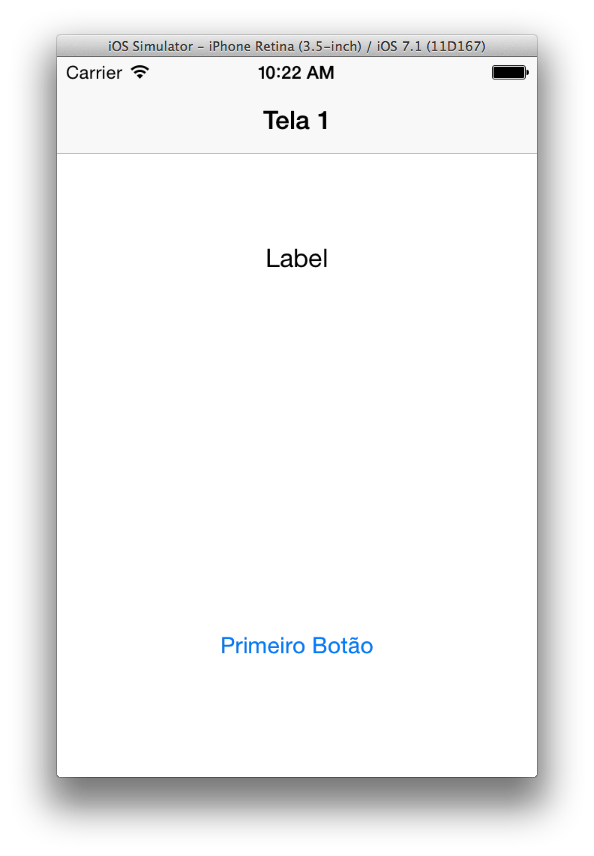
\includegraphics[width=.55\textwidth]{figuras/3/tela_novo_projeto_26.png}
  \caption{Aplicativo executando no iOS Simulator}
  \label{fig:app_executanto1}
\end{figure}

Podemos agora começar a adicionar funcionalidades com o código. Vamos criar outra \texttt{\textbf{IBAction}} bem simples para testar o comportamento do aplicativo com o simulador. Uma maneira mais prática para isso (ao invés de declarar a \texttt{\textbf{IBAction}} antes e depois conectá-la ao botão como feito com o \emph{mostrarMensagem}) é arrastar o botão para o código do arquivo.h segurando \emph{Ctrl}, escolher a opção \texttt{\textbf{IBAction}} e criar um nome para ela, como \texttt{\textbf{okTouched}}. A intenção da nossa \texttt{\textbf{IBAction}} é que os textos do botão e da label troquem quando clicarmos no botão.

\begin{figure}[H]
  \centering
  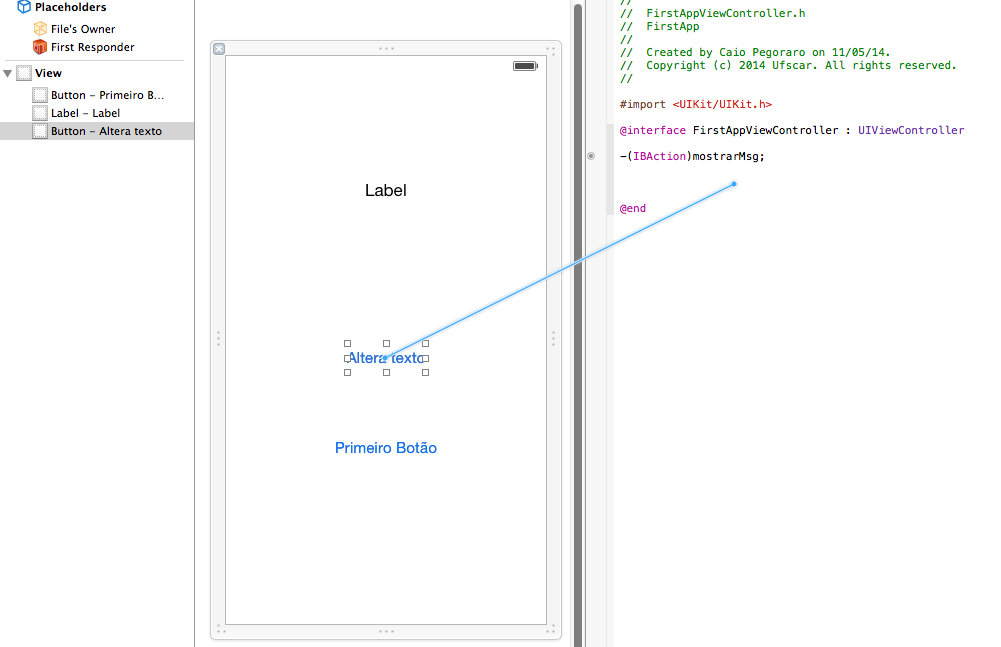
\includegraphics[width=.99\textwidth]{figuras/3/tela_novo_projeto_27.png}
  \caption{Adicionando uma \texttt{\textbf{IBAction}} diretamente no código}
  \label{fig:a}
\end{figure}

\begin{figure}[H]
  \centering
  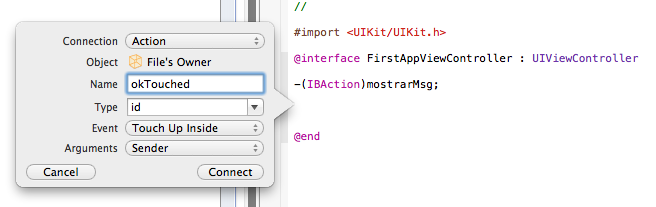
\includegraphics[width=.75\textwidth]{figuras/3/tela_novo_projeto_28.png}
  \caption{Nomeando a \texttt{\textbf{IBAction}}}
  \label{fig:a}
\end{figure}


Além da \texttt{\textbf{IBAction}} precisamos criar 2 \texttt{\textbf{IBOutlets}}, um para a label e outro para o novo botão, possibilitando que alterações sejam feitas nas propriedades (texto, visibilidade, etc.) dos objetos da interface através da manipulação dos objetos do código.
Da mesma forma que a \texttt{\textbf{IBAction}} anterior foi criada, é possível criar a \texttt{\textbf{IBOutlet}} segurando a tecla \emph{Ctrl} esquerdo e levando o mouse até o arquivo.h da classe da interface, o campo \emph{Connection} deve ser selecionado com \texttt{\textbf{IBOutlet}}.
Os nomes dos  \texttt{\textbf{IBOutlet}} devem ter ligação com os objetos da interface para facilitar o uso, o referente ao botão foi nomeado de \emph{botaoAlteraTexto} e da label de \emph{labelExemplo}.

\begin{figure}[H]
  \centering
  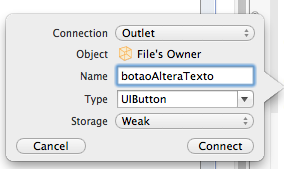
\includegraphics[width=.45\textwidth]{figuras/3/tela_novo_projeto_29.png}
  \caption{Adicionando a \texttt{\textbf{IBOutlet}} ao código}
  \label{fig:a}
\end{figure}

\begin{figure}[H]
  \centering
  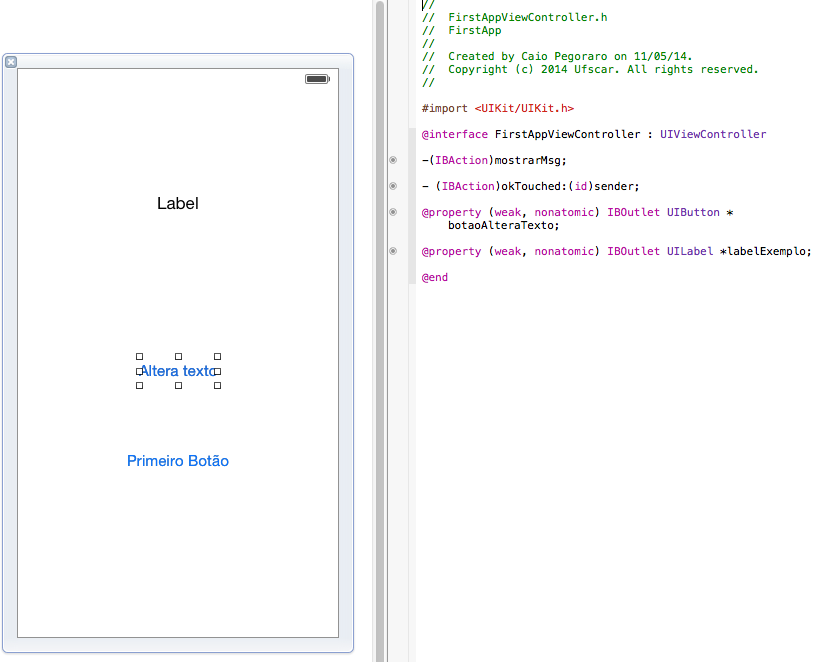
\includegraphics[width=.75\textwidth]{figuras/3/tela_novo_projeto_30.png}
  \caption{Estrutura do código com as \texttt{\textbf{IBOutlet's}} criadas}
  \label{fig:a}
\end{figure}


Veja que no código de implementação da classe da interface (arquivo .m) já será criado o esqueleto do método que será chamado, onde colocaremos nossa lógica.

\begin{listing}[H]
\begin{minted}[linenos=true,frame=lines,framesep=2mm,tabsize=2,numbersep=5pt]{objective-c}
- (IBAction)okTouched:(id)sender {
    
    NSString *aux = [[NSString alloc] 
    		initWithString:self.botaoAlteraTexto.currentTitle];
    
    [self.botaoAlteraTexto setTitle:self.labelExemplo.text 
    		forState:UIControlStateNormal];
    
    self.labelExemplo.text = aux;
}
\end{minted}
\caption{Implementação de uma \texttt{\textbf{IBAction}}}
\end{listing}


O código funciona como uma troca simples. Na linha 3 inicializamos uma variável local com o texto da label, na linha 6 chamamos o método da classe \texttt{\textbf{UIButton}} responsável por modificar o texto do botão pelo texto presente na label e no final o texto salvo do botão é atribuído à label.

Rode o aplicativo no simulador para verificar o funcionamento do botão.

\subsection{Manipulando a Navigation Controller}


Pensando agora na próxima tela, vamos preparar o código para a transição. Adicionamos um novo botão que servirá de chamada para a segunda tela, e criamos um \texttt{\textbf{IBOutlet}} e uma \texttt{\textbf{IBAction}} para ele. Colocaremos no método da \texttt{\textbf{IBAction}} a chamada para a segunda tela, que será através de um \emph{push} da tela na Navigation Controller.


Para chamar uma nova tela é preciso criar uma instância da \emph{View Controller} (uma nova interface) a ser chamada, no caso da SecondScreenViewController (que ainda não criamos), para então jogá-la na pilha com o método de \emph{push}, que recebe como parâmetro a instância criada. Crie um botão na primeira tela do aplicativo (\emph{FirstAppViewController.xib}) com o texto \emph{Ir para tela 2}.


\begin{figure}[H]
  \centering
  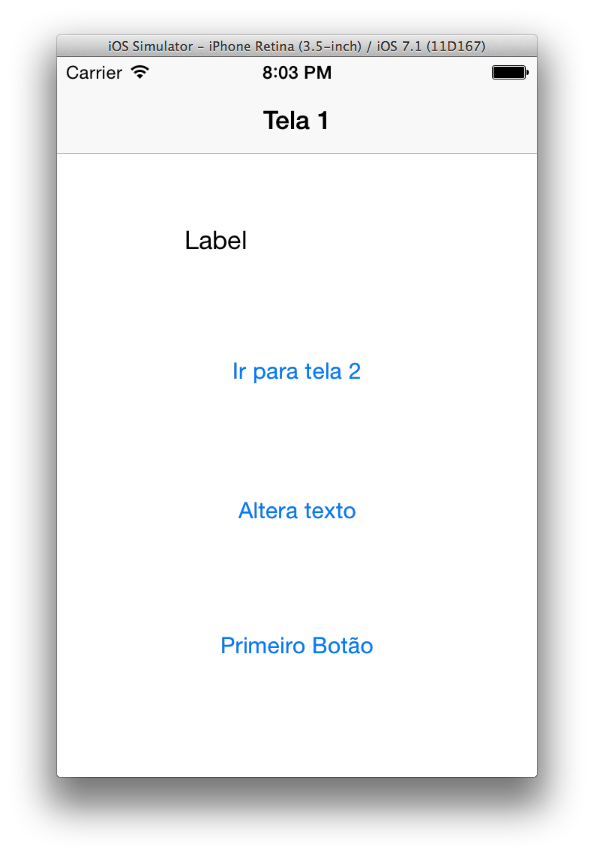
\includegraphics[width=.55\textwidth]{figuras/3/tela_novo_projeto_31.png}
  \caption{Primeira tela com o botão de chamada para segunda tela}
  \label{fig:a}
\end{figure}


Agora precisamos criar a segunda tela que será chamada, clique com direito na pasta do projeto e em \emph{New file}. Selecione \emph{Objective-C class} e clique em \emph{Next}, vamos dar o nome de \emph{SecondScreenViewController} e marcar a opção \emph{Also create a XIB file}.

\begin{figure}[H]
  \centering
  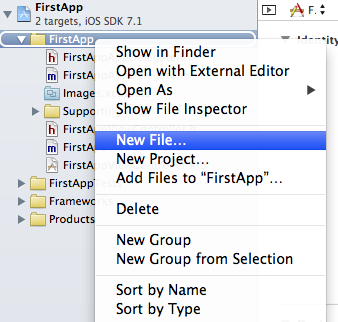
\includegraphics[width=.35\textwidth]{figuras/3/tela_novo_projeto_32.png}
  \caption{Criação da segunda tela do aplicativo}
  \label{fig:a}
\end{figure}

\begin{figure}[H]
  \centering
  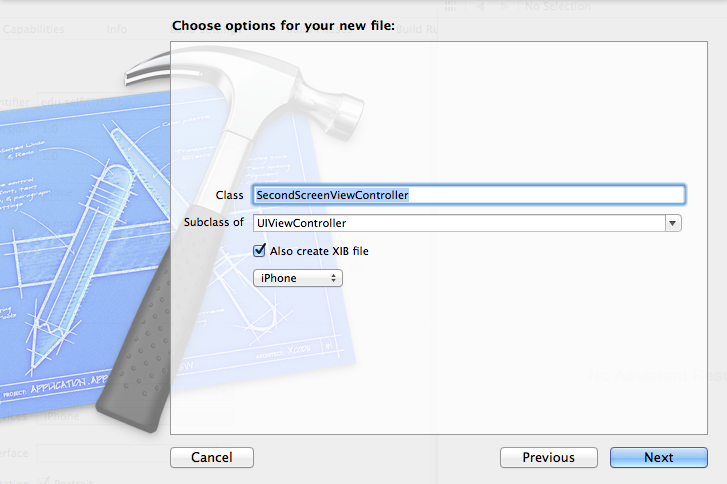
\includegraphics[width=.75\textwidth]{figuras/3/tela_novo_projeto_33.png}
  \caption{Configuração da segunda tela do aplicativo}
  \label{fig:a}
\end{figure}


A tela do projeto deve estar como a figura \ref{fig:app_com_duas_telas}.

\begin{figure}[H]
  \centering
  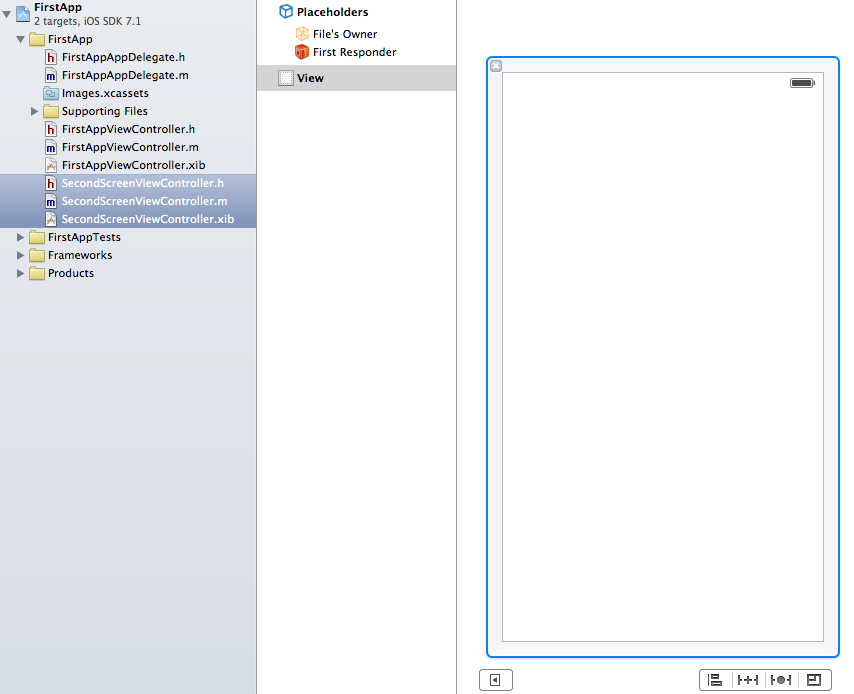
\includegraphics[width=.75\textwidth]{figuras/3/tela_novo_projeto_34.png}
  \caption{Aplicativo com as duas telas criadas}
  \label{fig:app_com_duas_telas}
\end{figure}


Nessa segunda tela vamos colocar uma \texttt{\textbf{UIImageView}}, arrastando da mesma forma que os outros objetos, e por enquanto mais um botão que fará a chamada de uma terceira tela.

\begin{figure}[H]
  \centering
  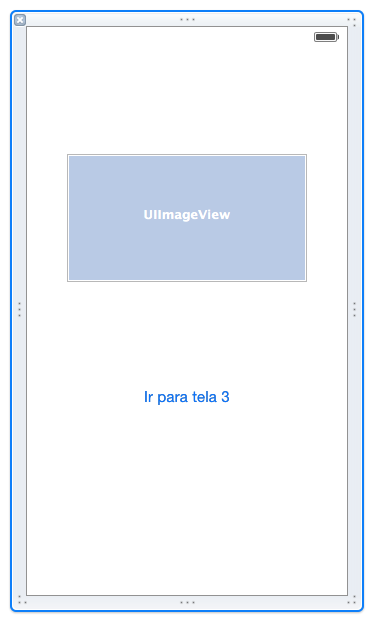
\includegraphics[width=.55\textwidth]{figuras/3/tela_novo_projeto_35.png}
  \caption{Tela 2 com \texttt{\textbf{UIImage}} ainda sem imagem definida}
  \label{fig:a}
\end{figure}


Devemos agora definir uma imagem para a \texttt{\textbf{UIImageView}}, mas antes devemos adicionar a imagem que queremos na pasta \emph{Supporting Files} do projeto. Para isso, basta clicar com o botão direito na pasta e selecionar a opção \emph{Add Files to "First App"...}, sendo \emph{"First App"} o nome dado ao projeto.

\begin{figure}[H]
  \centering
  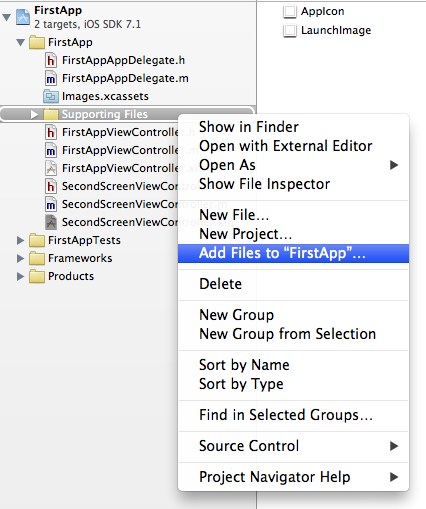
\includegraphics[width=.65\textwidth]{figuras/3/tela_novo_projeto_36.png}
  \caption{Adicionando arquivos ao projeto}
  \label{fig:a}
\end{figure}


Selecione uma imagem (nesse caso foi a de nome \emph{LogoDC.jpg}), agora temos a nova imagem disponível no \emph{Project Navigator}.

\begin{figure}[H]
  \centering
  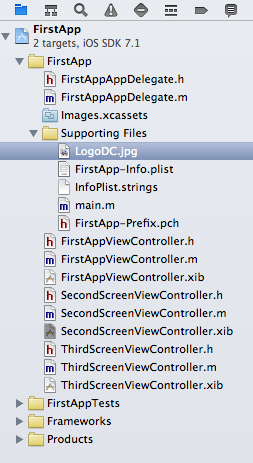
\includegraphics[scale=0.6]{figuras/3/tela_novo_projeto_50.png}
  \caption{Nova imagem adicionada ao projeto}
  \label{fig:a}
\end{figure}


Clicando no nome da imagem é possível alterar suas propriedades nesse projeto (as opções são exibidas no lado direito da tela do XCode). Altere a propriedade \emph{Type} de \emph{Relative to Group} para \emph{Relative to Project}, desse modo o caminho da imagem será relativo ao diretório onde se encontra o projeto.

\begin{figure}[H]
  \centering
  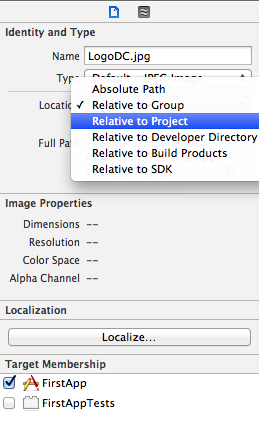
\includegraphics[scale=0.6]{figuras/3/tela_novo_projeto_51.png}
  \caption{Definindo o caminho da imagem relativo ao projeto}
  \label{fig:a}
\end{figure}


Adicionamos a imagem LogoDC.jpg contida no repositório deste turorial. Depois de adicionada,voltando à segunda tela do projeto (\emph{SeCondScreenViewController.xib}), selecionamos a \texttt{\textbf{UIImageView}} e selecionamos a imagem para ser exibida.

\begin{figure}[H]
  \centering
  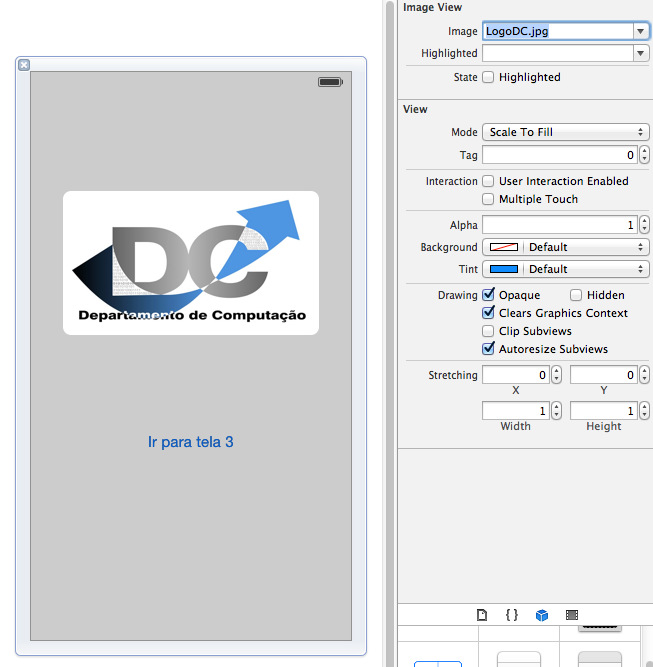
\includegraphics[width=.75\textwidth]{figuras/3/tela_novo_projeto_37.png}
  \caption{Selecionando a nova imagem}
  \label{fig:a}
\end{figure}

Com a segunda tela criada, voltemos para a primeira (\emph{FirstAppViewController.xib}) para configurar o botão \emph{Ir para tela 2}. Para isso vamos criar uma \texttt{\textbf{IBAction}}, segurando a tecla \emph{Ctrl} esquerdo clique no botão e arraste para a parte de código do arquivo \emph{FirstAppViewController.h}.

\begin{figure}[H]
  \centering
  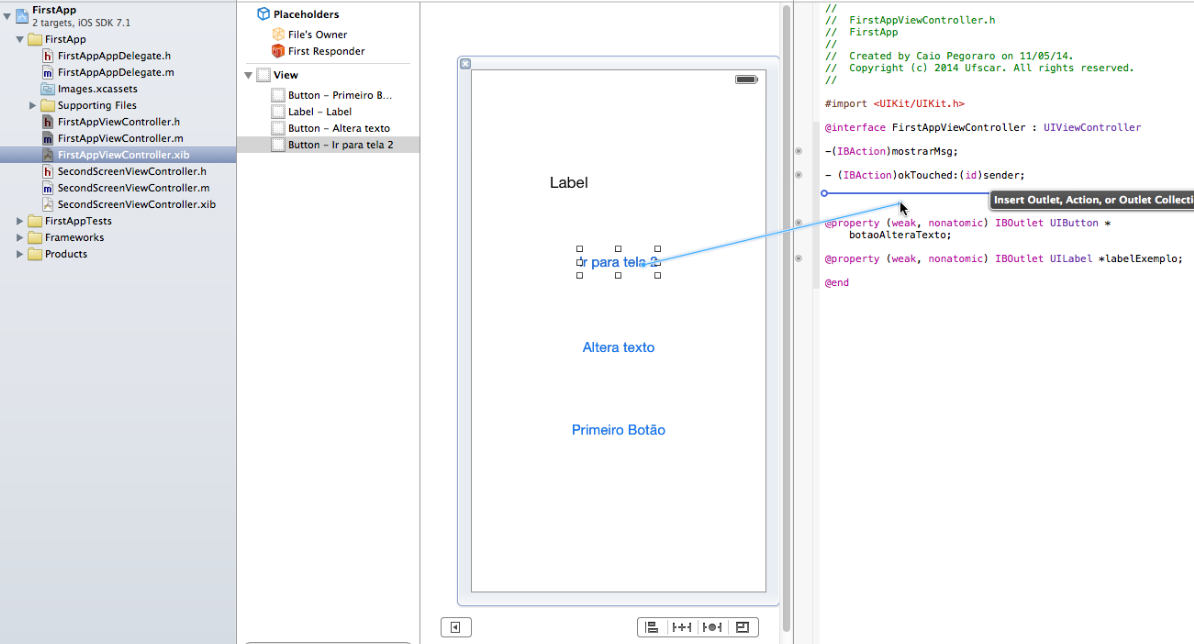
\includegraphics[width=.99\textwidth]{figuras/3/tela_novo_projeto_38.png}
  \caption{Criando uma \texttt{\textbf{IBAction}} diretamente}
  \label{fig:a}
\end{figure}

\begin{figure}[H]
  \centering
  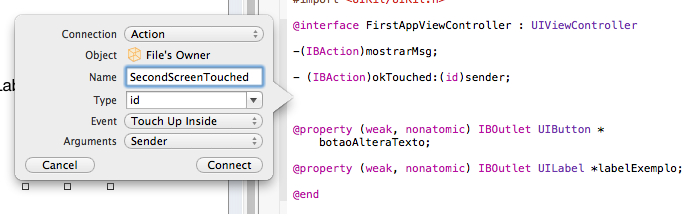
\includegraphics[width=.75\textwidth]{figuras/3/tela_novo_projeto_39.png}
  \caption{Definindo a propriedade da \texttt{\textbf{IBAction}}}
  \label{fig:a}
\end{figure} 

Com a \texttt{\textbf{IBAction}} criada, vamos para o arquivo \emph{FirstAppViewController.m} onde já foi criado automaticamente o esqueleto dessa ação. Para chamar a segunda tela primeiramente inclua nesse arquivo .m a importação da classe referente à segunda tela:

\begin{listing}[H]
\begin{minted}[linenos=true,frame=lines,framesep=2mm,tabsize=2,numbersep=5pt]{objective-c}
#import "SecondScreenViewController.h"
\end{minted}
\caption{Importando a classe de uma nova tela}
\end{listing}


Em seguida deixe o método da \texttt{\textbf{IBAction}} como abaixo:

\begin{listing}[H]
\begin{minted}[linenos=true,frame=lines,framesep=2mm,tabsize=2,numbersep=5pt]{objective-c}
- (IBAction)SecondScreenTouched:(id)sender {
    SecondScreenViewController *SecondViewController = 
    			[[SecondScreenViewController alloc] 
			initWithNibName:@"SecondScreenViewController" bundle:nil];
    
    [self.navigationController pushViewController: 
    						SecondViewController animated:true];
}
\end{minted}
\caption{Chamada da tela 2 do aplicativo}
\end{listing}


Na linha 2 inicializamos a \emph{View Controller} e na linha 6 adicionamos a \emph{View Controller} à pilha da \emph{Navigation Controller}.


Agora vá até o arquivo .m da segunda tela (\emph{SecondScreenViewController.m}) e deixe o método \emph{- (void)viewDidLoad} da seguinte forma:

\begin{listing}[H]
\begin{minted}[linenos=true,frame=lines,framesep=2mm,tabsize=2,numbersep=5pt]{objective-c}
- (void)viewDidLoad
{
    [super viewDidLoad];
    self.navigationItem.title = @"Tela 2";
}
\end{minted}
\caption{Chamada de uma nova tela}
\end{listing}


O código da linha 4 serve para dar um título para a tela que será exibido na \emph{Navigation controller}.

Rode o aplicativo para testar a função, quando estiver na tela 2 é possível retornar à tela 1 através da \emph{Navigation controller} no topo da tela.

\begin{figure}[H]
  \centering
  \includegraphics[width=.55\textwidth]{figuras/3/tela_novo_projeto_40.png}
  \caption{Segunda tela do aplicativo}
  \label{fig:a}
\end{figure} 


Para dar funcionalidade ao botão \emph{Ir para tela 3}, crie a terceira tela com o nome \emph{ThirdScreenViewController}, seguindo o exemplo, e faça a chamada da mesma forma que foi feito na primeira tela. Faça os testes e verifique o funcionamento. É possível retornar às telas anteriores, pois a \emph{Navigation Controller} cria um botão de retorno automaticamente.

\subsection{Trocando informação entre telas}

Ao inicializarmos uma instância de uma \emph{View Controller}, podemos atribuir valores às suas \emph{Properties} antes de fazer o \emph{push} da tela. Dessa forma bem simples, é possível levar informação de uma tela existente para uma tela nova, podendo exibir ou tratar esses dados convenientemente na \emph{View Controller} da próxima tela. Para exemplificar, vamos criar um campo de texto na segunda tela e exibir o seu conteúdo em um rótulo (\emph{label}) na terceira tela.

Para isso vamos precisar de um campo de texto na segunda tela, de um rótulo na terceira tela, e de uma variável do tipo string na terceira tela (ThirdScreenViewController.h), onde vamos armazenar o conteúdo do campo de texto. Além disso, também é preciso editar a \texttt{\textbf{IBAction}} que faz a chamada da terceira tela pelo botão.

A \texttt{\textbf{Property}} da string é criada no arquivo de header da classe da terceira tela da seguinte forma:

\begin{listing}[H]
\begin{minted}[linenos=true,frame=lines,framesep=2mm,tabsize=2,numbersep=5pt]{objective-c}
@property (nonatomic, strong) NSString *textLabel;
\end{minted}
\caption{Propriedade do tipo \emph{NSString}}
\end{listing}

Além da variável NSString é necessário criar o \texttt{\textbf{IBOutlet}} da \emph{label} da tela 3. Dessa forma o valor será passado da tela 2 para a variável NSString e então passado para a label da interface.

\begin{figure}[H]
  \centering
  \includegraphics[width=.99\textwidth]{figuras/3/tela_novo_projeto_45.png}
  \caption{Criação do \texttt{\textbf{IBOutlet}} da caixa de texto da tela 3}
  \label{fig:a}
\end{figure} 

\begin{figure}[H]
  \centering
  \includegraphics[width=.75\textwidth]{figuras/3/tela_novo_projeto_46.png}
  \caption{Configuração do \texttt{\textbf{IBOutlet}} da caixa de texto da tela 3}
  \label{fig:a}
\end{figure} 
 

Na segunda tela deve ser adicionado um \emph{text} que será utilizado para digitar o texto, em seguida criado um \texttt{\textbf{IBOutlet}} para esse \emph{text}.

\begin{figure}[H]
  \centering
  \includegraphics[width=.99\textwidth]{figuras/3/tela_novo_projeto_42.png}
  \caption{Criação da \texttt{\textbf{IBOutlet}} da caixa de texto}
  \label{fig:a}
\end{figure} 

\begin{figure}[H]
  \centering
  \includegraphics[width=.75\textwidth]{figuras/3/tela_novo_projeto_43.png}
  \caption{Configuraçao da \texttt{\textbf{IBOutlet}} da caixa de texto}
  \label{fig:a}
\end{figure} 


\begin{figure}[H]
  \centering
  \includegraphics[width=.99\textwidth]{figuras/3/tela_novo_projeto_44.png}
  \caption{Tela 2 e seus atributos. Repare nas as ligações dos \texttt{\textbf{IBOutlets}} com a interface.}
  \label{fig:a}
\end{figure}

E o método com a chamada da terceira tela será semelhante, apenas com a adição da passagem da variável na linha 7 do código a seguir.

\begin{listing}[H]
\begin{minted}[linenos=true,frame=lines,framesep=2mm,tabsize=2,numbersep=5pt]{objective-c}
- (IBAction)ThirdScreenTouched:(id)sender {

    ThirdScreenViewController *ThirdViewController =
    [[ThirdScreenViewController alloc]
     initWithNibName:@"ThirdScreenViewController" bundle:nil];
    
    ThirdViewController.textLabel = self.labelTexto2.text;
    
    [self.navigationController pushViewController:
    						ThirdViewController animated:true];
    
}
\end{minted}
\caption{Chamada de uma nova tela enviando uma variável}
\end{listing}


Além disso, precisamos tratar o conteúdo da variável na classe da terceira tela. Vamos verificar no método \texttt{\textbf{viewDidLoad}} presente no arquivo \emph{ThirdScreenViewController.m} o conteúdo da variável que recebeu o dado da segunda tela.

\begin{listing}[H]
\begin{minted}[linenos=true,frame=lines,framesep=2mm,tabsize=2,numbersep=5pt]{objective-c}
- (void)viewDidLoad
{
    [super viewDidLoad];
    self.navigationItem.title = @"Tela 3";
    
    if (![self.textLabel isEqualToString:@""]){
        self.labelTela3.text = self.textLabel;
    }
    else {
        self.labelTela3.text = @"Em branco";
    }
}
\end{minted}
\caption{Tratamento da variável recebida na próxima tela}
\end{listing}


De uma forma bem simples, verificamos o conteúdo da string recebida na linha 6 e a atribuimos para o conteúdo do rótulo na linha 7 ou 10, de acordo com a condição.

Note que há ainda um problema gráfico: após a edição do campo de texto na segunda tela, o teclado sobre mas não abaixa automaticamente, mas deixaremos assim por enquanto. Tente posicionar o campo de texto e o botão de forma que o teclado não os cubra, apenas para verificar o funcionamento do código. Resolveremos o problema do teclado mais a frente.

A imagem a seguir mostra a segunda tela no simulador.

\begin{figure}[H]
  \centering
  \includegraphics[width=.55\textwidth]{figuras/3/tela_novo_projeto_47.png}
  \caption{Tela 2 completa}
  \label{fig:a}
\end{figure}

\subsection{O uso do protocolo Delegate}

O protocolo \texttt{\textbf{Delegate}} é uma das ferramentas mais importantes do Objective-C. Na execução do código de um objeto, este não tem como ter acesso ao código do objeto que o instanciou. Com o uso do \texttt{\textbf{Delegate}} um objeto pode enviar dados para um segundo objeto que enxerga o primeiro mas não pode ser enxergado por ele. Assim é possível determinar que a partir de um evento ou uma condição, será enviada uma mensagem, que pode ser uma notificação ou um dado, a partir de um método \texttt{\textbf{Delegate}} que vai saber como e onde encontrar o destino dessa mensagem.

Veremos dois exemplos de uso do \texttt{\textbf{Delegate}} no nosso aplicativo. No primeiro usaremos um método já pronto, que será responsável por enviar o aviso para o teclado de que o campo de texto já terminou de ser usado e ele agora deve desaparecer. No segundo vamos implementar um método para enviar uma string da terceira tela para a tela que a chamou, no nosso caso a segunda tela.

Utilizar o \texttt{\textbf{Delegate}} já implementado do \texttt{\textbf{UITextField}} é bem simples. Fazemos uma referência no header (arquivos .h) de todas as classes em que utilizarmos o teclado em um \texttt{\textbf{UITextField}}, no caso a segunda e terceira tela (SecondScreenViewController e ThirdScreenViewController). Fazemos dessa forma:

\begin{listing}[H]
\begin{minted}[linenos=true,frame=lines,framesep=2mm,tabsize=2,numbersep=5pt]{objective-c}
@interface SecondScreenViewController :
           UIViewController <UITextFieldDelegate>
\end{minted}
\caption{Referência ao \emph{UITextFieldDelegate} na declaração da classe}
\end{listing}


A referência a um \texttt{\textbf{Delegate}} vem sempre entre os símbolos < e > na declaração da classe, separando por vírgula dentro da chave se houver mais de um. Após isso, precisamos apenas atribuir o \texttt{\textbf{Delegate}} à classe no \texttt{\textbf{viewDidLoad}} (encontrado nos arquivos.m) das classes em que utilizaremos o\\ \texttt{\textbf{UITextFieldDelegate}}.

\begin{listing}[H]
\begin{minted}[linenos=true,frame=lines,framesep=2mm,tabsize=2,numbersep=5pt]{objective-c}
self.nameTextField.delegate = self;
\end{minted}
\caption{Definição do \emph{delegate}}
\end{listing}

Pronto, agora é possível que o objeto \texttt{\textbf{UITextField}}, que foi instanciado na classe da tela e consequentemente não enxerga os elementos dessa classe, como o teclado, envie informações à mesma. No caso, queremos que o teclado seja dispensado no momento que terminarmos de editar o campo de texto, e quando isso ocorre há um método a ser chamado. Vamos implementar este método com a lógica que queremos no arquivo de implementação da classe.

\begin{listing}[H]
\begin{minted}[linenos=true,frame=lines,framesep=2mm,tabsize=2,numbersep=5pt]{objective-c}
- (BOOL)textFieldShouldReturn:(UITextField *)textField {
    
    if (textField == self.nameTextField) {
        [textField resignFirstResponder];
    }
    
    return YES;
}
\end{minted}
\caption{Implementação de métodos do \emph{UITextFieldDelegate}}
\end{listing}


Este código verifica na linha 3 se o objeto \texttt{\textbf{UITextField}} que chamou o método é o mesmo objeto instanciado na classe, no caso o \texttt{\textbf{nameTextField}}. Assim, quando há mais de um \texttt{\textbf{UITextField}}, podemos definir comportamentos diferentes para cada um apenas fazendo essa verificação. Execute o projeto e faça o teste, agora o teclado deve sumir quando o campo de texto não está selecionado.

No exemplo anterior, fizemos o uso de um \texttt{\textbf{Delegate}} existente. Agora vamos implementar um novo \texttt{\textbf{Delegate}} a partir do zero para determinar o envio de informações de uma tela para a tela que a chamou. Vamos definir o \texttt{\textbf{Delegate}} na classe da terceira tela, e usar o método na segunda. Criamos um \texttt{\textbf{Protocol}} no header da classe, e dentro inserimos os métodos do \texttt{\textbf{Delegate}}, que no caso será apenas um, que terá a função de enviar como parâmetro o conteúdo de um campo de texto da terceira tela. Ficará assim:

\begin{listing}[H]
\begin{minted}[linenos=true,frame=lines,framesep=2mm,tabsize=2,numbersep=5pt]{objective-c}
@protocol MessageDelegate <NSObject>

-(void)sendMessageFromTextField:(NSString*)message;

@end
\end{minted}
\caption{Declaração de um método \emph{Delegate}}
\end{listing}


Esta é a declaração de um protocolo \texttt{\textbf{Delegate}}. O título é declarado entre \texttt{\textbf{•}{@protocol}} e \texttt{\textbf{<NSObject>}}, e entre a declaração do título e \texttt{\textbf{@end}} é feita a declaração de todos os métodos desse \texttt{\textbf{Delegate}}.

Então criamos uma propriedade no header para o \texttt{\textbf{Delegate}} que criamos, que tem o nome \texttt{\textbf{MessageDelegate}}.

\begin{listing}[H]
\begin{minted}[linenos=true,frame=lines,framesep=2mm,tabsize=2,numbersep=5pt]{objective-c}
@property (assign, nonatomic) id <MessageDelegate> delegate;
\end{minted}
\caption{Declaração da propriedade do \emph{Delegate} criado}
\end{listing}


O que fizemos aqui foi criar a declaração de um \texttt{\textbf{Delegate}}, como fazemos com uma classe, e então instanciamos um objeto do tipo do \texttt{\textbf{Delegate}} que criamos. Este objeto servirá de referência para que outras classes possam implementar e utilizar os métodos criados pelo \texttt{\textbf{Delegate}}.

Definimos o \texttt{\textbf{Delegate}} e seu método, agora basta definir onde será a chamada do método. Criaremos um \emph{Text field} e ligaremos através de uma \texttt{\textbf{IBOUtlet}} chamada de \emph{textoTerceiraTela} e um botão na terceira tela , ligado a uma \texttt{\textbf{IBAction}} de nome \texttt{\textbf{sendMessage}}, nesta \texttt{\textbf{IBAction}} ficará a chamada para o método do \texttt{\textbf{Delegate}}.

\begin{listing}
\begin{minted}[linenos=true,frame=lines,framesep=2mm,tabsize=2,numbersep=5pt]{objective-c}
- (IBAction)sendMessage:(id)sender {
    
    [self.delegate sendMessageFromTextField:
                   self.textoTerceiraTela.text];
}
\end{minted}
\caption{Chamada do método criado no \emph{Delegate}}
\end{listing}

Este é o método da \texttt{\textbf{IBAction}} que criamos, e é acionado quando o botão "Enviar Mensagem" é tocado. Dentro dele fazemos a chamada do método \texttt{\textbf{sendMessageFromTextField}} definido no \texttt{\textbf{MessageDelegate}}, que vai buscar a implementação do método em qualquer classe que tenha referenciado o \texttt{\textbf{MessageDelegate}}.

\begin{figure}[H]
  \centering
  \includegraphics[width=.55\textwidth]{figuras/3/tela_novo_projeto_49.png}
  \caption{Tela 3 com o botão para enviar mensagem}
  \label{fig:a}
\end{figure}


Isso determina que ao apertarmos o botão da tela 3, o método do \texttt{\textbf{Delegate}} que criamos será chamado recebendo o conteúdo do campo como parâmetro. Para receber esse conteúdo na segunda tela, faremos como no caso do teclado, implementando o método criado no \texttt{\textbf{Delegate}} com o comportamento que for desejado.

Na segunda tela, faremos o mesmo processo que fizemos com o \texttt{\textbf{Delegate}} do \texttt{\textbf{UITextField}}. Adicionamos a referência ao nosso \texttt{\textbf{Delegate}} ao header (SecondScreenViewController.h).\\

\begin{listing}[H]
\begin{minted}[linenos=true,frame=lines,framesep=2mm,tabsize=2,numbersep=5pt]{objective-c}
@interface SecondScreenViewController : UIViewController
           <UITextFieldDelegate, MessageDelegate>
\end{minted}
\caption{Referência ao \emph{Delegate} criado}
\end{listing}


Adicione também a importação da Tela 3 ao arquivo \emph{SecondScreenViewController.h}:

\begin{listing}[H]
\begin{minted}[linenos=true,frame=lines,framesep=2mm,tabsize=2,numbersep=5pt]{objective-c}
#import "ThirdScreenViewController.h"
\end{minted}
\caption{Importação da Tela 3}
\end{listing}


No método em que é chamada a terceira tela, atribuímos o nosso \texttt{\textbf{Delegate}} à classe da segunda tela, logo após a instanciação.

\begin{listing}[H]
\begin{minted}[linenos=true,frame=lines,framesep=2mm,tabsize=2,numbersep=5pt]{objective-c}
- (IBAction)ThirdScreenTouched:(id)sender {

    ThirdScreenViewController *ThirdViewController =
    [[ThirdScreenViewController alloc]
     initWithNibName:@"ThirdScreenViewController" bundle:nil];
    
    ThirdViewController.textLabel = self.labelTexto2.text;
    
    ThirdViewController.delegate = self;
    
    [self.navigationController pushViewController:ThirdViewController 
    													animated:true];
}
\end{minted}
\caption{Atribuição do \emph{Delegate} criado}
\end{listing}


Na linha 9 temos a adição da referência da instância do \texttt{\textbf{MessageDelegate}} da tela 3 para a tela 2.

Tudo pronto, agora basta implementar o método. Nossa intenção é que a segunda tela retorne exibindo o texto recebido da terceira tela no campo de texto, ou seja, precisamos chamar a terceira tela e atribuir o texto recebido por parâmetro ao campo de texto \texttt{\textbf{nameTextField}}. Deve ficar assim no arquivo \emph{SecondViewController.m}:

\begin{listing}[H]
\begin{minted}[linenos=true,frame=lines,framesep=2mm,tabsize=2,numbersep=5pt]{objective-c}
-(void)sendMessageFromTextField:(NSString *)message { 

[self.navigationController popToViewController:self 
										animated:YES];
										
    self.textoSegundaTela.text = message;
}
\end{minted}
\caption{Implementação do método do \emph{Delegate} criado}
\end{listing}


Na linha 3 chamamos a tela 3 para a \emph{Navigation Controller}, e na linha 6 salvamos a mensagem que escrevemos como conteúdo do campo de texto criado na tela 3, na segunda tela foi criado um \emph{Text field} ligado através de uma \texttt{\textbf{IBOutlet}} chamada de \emph{textoSegundaTela} .

\section{Criando uma agenda}

Entre os tipos de \emph{Views} mais utilizadas no iOS, temos as tabelas. Qualquer tela exibindo informações bem divididas como playlist de músicas, lista contatos, ou informações estruturadas em linhas, é do tipo \texttt{\textbf{UITableView}} se for uma \emph{View}, ou \texttt{\textbf{UITableViewController}} se for uma controladora. Como já explicado, se for preciso apenas exibir informações estáticas sem interação com o usuário, criamos uma classe herdando de \texttt{\textbf{UITableView}}, porém na maioria dos casos vamos precisar de tabelas com dados dinâmicos e possibilidade de interação por toque, então criamos um classe herdando de \texttt{\textbf{UITableViewController}}.

A classe \texttt{\textbf{UITableViewController}} possui diversos métodos para gerenciar o comportamento de uma tabela. Desde o básico para defininção do número de seções, linhas por seções e o conteúdo de cada linha, até o ajuste das ações para tipos diferentes de toque, como um toque único ou um \emph{slide} na linha para obter novas opções.

Vamos implementar um exemplo simples de uma lista de contatos, exibindo-os em ordem alfabética a partir de um pré-determinado \emph{array} de objetos do tipo \texttt{\textbf{Contato}}, que será a classe modelo que criaremos para contatos com informações como nome completo e número.

\begin{figure}[H]
  \centering
  \includegraphics[width=.75\textwidth]{figuras/apple_table_view_controller_contatos.png}
  \caption{Exemplo de tela com lista de contatos que chama tela com lista de atributos}
  \label{fig:a}
\end{figure}

É interessante que você acompanhe o tutorial junto com a documentação da Apple sobre \texttt{\textbf{UITableViewController}}, e no final busque novos tipos de interação com o usuário e customização da tabela. Não é a toa que essa estrutura é tão explorada nos aplicativos, há uma gama muito grande de possibilidades para seu uso.

Crie um novo projeto da mesma forma que fizemos com o primeiro aplicativo, e coloque "Table" como nome. Agora abra o arquivo \texttt{\textbf{TableViewController.m}} e na declaração da classe adicione \texttt{\textbf{<UITableViewDataSource,UITableViewDelegate>}}.

\begin{listing}[H]
\begin{minted}[linenos=true,frame=lines,framesep=2mm,tabsize=2,numbersep=5pt]{objective-c}
@interface TableViewController : UIViewController
             <UITableViewDataSource,UITableViewDelegate>
\end{minted}
\caption{Declarando o controle de uma \emph{UITableView}}
\end{listing}


Assim teremos a possibilidade de sobrescrever diversos métodos da \texttt{\textbf{UITableView}} que já são chamados pela controladora para gerenciar o comportamento e as configurações da tabela.

Métodos como esse:

\begin{listing}
\begin{minted}[linenos=true,frame=lines,framesep=2mm,tabsize=2,numbersep=5pt]{objective-c}
- (NSInteger)tableView:(UITableView *)tableView
 numberOfRowsInSection:(NSInteger)section
\end{minted}
\caption{Método utilizado por uma \emph{UITableView}}
\end{listing}


Que retorna o número de linhas por seção. E esse:

\begin{listing}
\begin{minted}[linenos=true,frame=lines,framesep=2mm,tabsize=2,numbersep=5pt]{objective-c}
- (UITableViewCell *)tableView:(UITableView *)tableView
         cellForRowAtIndexPath:(NSIndexPath *)indexPath
\end{minted}
\caption{Mais um método utilizado por uma \emph{UITableView}}
\end{listing}


Que é chamado no carregamento de cada célula da tabela e retorna um objeto \texttt{\textbf{UITableViewCell}} que contém as definições dessa celula, como texto, imagem de fundo, ou uma imagem miniatura. O endereço da célula é obtido pelo parâmetro \texttt{\textbf{indexPath}}, que contém dois valores: a seção (\texttt{\textbf{section}}) e a linha (\texttt{\textbf{row}}).

Vamos carregar os dados dos contatos a partir de uma property list chamada \texttt{\textbf{contatos.plist}} já criada e presente no repositório. Adicione este arquivo no projeto e abra-o para entender como os contatos estão estruturados. A ideia é dividir os contatos pela letra inicial, tornando cada letra existente uma chave primária para a estrutura. Dessa forma podemos montar esses dados em um dicionário e facilitar a busca e a ordenação dos contatos.

\subsection{Classe de modelo dos contatos}


Antes dessa leitura, é preciso criar uma classe modelo para o contato. A classe é simples, vai conter apenas nome, sobrenome, e número. Para isso, basta criar um novo arquivo da mesma que fizemos até agora, herdando simplesment de \texttt{\textbf{NSObject}}. Usaremos o nome \texttt{\textbf{DataContato}}.

No arquivo \texttt{\textbf{DataContato.h}} colocaremos apenas as 3 propriedades da classe, e um método construtor.

\begin{listing}[H]
\begin{minted}[linenos=true,frame=lines,framesep=2mm,tabsize=2,numbersep=5pt]{objective-c}
@interface DataContato : NSObject

@property (nonatomic, retain) NSString *firstName;
@property (nonatomic, retain) NSString *lastName;
@property (nonatomic, retain) NSString *numero;

- (id)initWithFirstName:(NSString *)aFirstName
               lastName:(NSString *)aLastName
                 numero:(NSString *)aNumero;

@end
\end{minted}
\caption{Declaração do modelo para contatos}
\end{listing}


E no arquivo \texttt{\textbf{DataContato.m}} colocamos a implementação do construtor.

\begin{listing}[H]
\begin{minted}[linenos=true,frame=lines,framesep=2mm,tabsize=2,numbersep=5pt]{objective-c}
@implementation DataContato

- (id)init
{
    return [self initWithFirstName:@"N/A"
                          lastName:@"N/A"
                            numero:@"N/A"];
}

- (id)initWithFirstName:(NSString *)aFirstName
               lastName:(NSString *)aLastName
                 numero:(NSString *)aNumero;
{    
    self.firstName = aFirstName;
    self.lastName = aLastName;
    self.numero = aNumero;
    
    return self;
}

@end
\end{minted}
\caption{Construtores do modelo de contatos}
\end{listing}

\subsection{Organização da estrutura}


Com o modelo pronto, podemos montar o arquivo \texttt{\textbf{contato.plist}} em um dicionário de uma forma que os dados tenham sentido. É preciso importar a classe em \texttt{\textbf{TableViewController.h}} e criar as propriedades e métodos que utilizaremos para gerenciar a estrutura dos contatos e orderná-los.

Em um projeto maior, o mais correto seria implementar o gerenciamento e lógica da estrutura de dados em uma classe separada, para manter o código organizado. Mas por enquanto vamos colocar a lógica na \texttt{\textbf{TableViewController}} para deixar mais simples o entendimento.

\begin{listing}[H]
\begin{minted}[linenos=true,frame=lines,framesep=2mm,tabsize=2,numbersep=5pt]{objective-c}
#import "DataContato.h"

@interface TableViewController : UIViewController 
           <UITableViewDataSource,UITableViewDelegate>

@property (nonatomic, retain) NSMutableDictionary *dictionary;
@property (nonatomic, retain) NSMutableArray *keysArray;
@property (nonatomic, retain) NSMutableArray *contatoObjArray;

- (void) setDictionaryArray;
- (void) sortObjArray:(NSMutableArray *)arrayObj;

@end
\end{minted}
\caption{Declaração das propriedades da tabela}
\end{listing}


A propriedade \texttt{\textbf{dictionary}} vai ser o nosso dicionário, contendo todos os dados do arquivo \texttt{\textbf{contatos.plist}}, desordenados e sem significado. Em \texttt{\textbf{keysArray}} salvaremos um \emph{array} com as primeiras letras dos contatos, assim podemos buscar os dados em \texttt{\textbf{dictionary}} para enfim transformá-los em objetos \texttt{\textbf{DataContato}}, e salvá-los em \texttt{\textbf{ContatoObjArray}}, divididos entre as letras.

Agora vamos para o arquivo de implementação definir nosso método \texttt{\textbf{viewDidLoad}}.

\begin{listing}[H]
\begin{minted}[linenos=true,frame=lines,framesep=2mm,tabsize=2,numbersep=5pt]{objective-c}
- (void)viewDidLoad
{
    [super viewDidLoad];
    
    self.navigationItem.title = @"Contatos";
    
    NSString *filePath = [[NSBundle mainBundle]
    					pathForResource:@"contatos"
    					ofType:@"plist"];
    
    self.dictionary = [[NSMutableDictionary alloc]
    				   initWithContentsOfFile:filePath];
    
    [self setDictionaryArray];
}
\end{minted}
\caption{Implementação da lista de contatos}
\end{listing}


Nesse código, primeiro damos à tela o título \emph{Contatos}, e então vamos montar o endereço do arquivo \texttt{\textbf{contatos.plist}} na variável \texttt{\textbf{filePath}}. Podemos então inicializar a propriedade \texttt{\textbf{dictionary}} com o conteúdo desse endereço. Por último chamamos o método \texttt{\textbf{setDictionaryArray}}, que será onde montaremos a estrutura dos contatos utilizando as chaves primárias e a classe \texttt{\textbf{DataContato}}.

Agora vamos montar o método \texttt{\textbf{setDictionaryArray}} por partes. Vamos primeiro separar as chaves primárias e ordená-las utilizando um objeto \texttt{\textbf{NSSortDescriptor}}:

\begin{listing}[H]
\begin{minted}[linenos=true,frame=lines,framesep=2mm,tabsize=2,numbersep=5pt]{objective-c}
NSMutableArray *tmpKey, *tmpContato;
    NSString *firstNameAux, *lastNameAux, *numeroAux;
    
    NSSortDescriptor *sort = [NSSortDescriptor
                              sortDescriptorWithKey:nil
                                          ascending:YES];
    
    self.keysArray = [[NSMutableArray alloc] initWithArray:
                                    [self.dictionary allKeys]];
    [self.keysArray sortUsingDescriptors:
                               [NSArray arrayWithObject:sort]];
    
    int countKeys = [self.keysArray count];

    NSMutableArray *arrayObj = [[NSMutableArray alloc] init];
\end{minted}
\caption{Ordenação das letras iniciais}
\end{listing}


Este código mostra um modo mais simples de ordenação de um \texttt{\textbf{NSArray}} 
com um \texttt{\textbf{NSSortDescriptor}}. Criamos o objeto \texttt{\textbf{sort}} e setamos que a ordenação vai ser ascendente, então salvamos em \texttt{\textbf{keysArray}} todas as chaves de \texttt{\textbf{dictionary}} utilizando o método \texttt{\textbf{allKeys}} de \texttt{\textbf{NSDictionary}}. Por fim fazemos a ordenação de \texttt{\textbf{keysArray}} com o método \texttt{\textbf{sortUsingDescriptors}}, onde mandamos como parâmetro um \texttt{\textbf{NSArray}} criado com o \texttt{\textbf{sort}}.

Sempre que vamos fazer uma ordenação de um \texttt{\textbf{NSArray}}, devemos criar um ou mais objeto \texttt{\textbf{NSSortDescriptor}} (podemos ter mais de um fato de ordenação, como veremos mais a frente) e criamos um novo\texttt{\textbf{NSArray}} contendo esses objetos. Com o \texttt{\textbf{NSArray}} a ser ordenado e o \texttt{\textbf{NSArray}} de ordenação, já temos tudo que é preciso para o método resolver o problema.

Agora continuamos com o método, e faremos um laço para separar os contatos de cada letra, utilizando métodos do \texttt{\textbf{NSDictionary}} para obter o conteúdo de cada chave. E dentro mais um laço para separar os dados de cada contato. Assim, podemos criar novas instâncias de \texttt{\textbf{DataContato}} com os dados obtidos da estrutura de \texttt{\textbf{dictionary}}.

\begin{listing}[H]
\begin{minted}[linenos=true,frame=lines,framesep=2mm,tabsize=2,numbersep=5pt]{objective-c}
for (int i=0; i<countKeys; i++)
    {
	 tmpKey = [[NSMutableArray alloc] init];
        tmpKey = [NSMutableArray arrayWithArray:
                  [self.dictionary objectForKey:
                          [self.keysArray objectAtIndex:i]]];
        
        NSMutableArray *arrayObjAux = [[NSMutableArray alloc] init];
        
        for (int j=0; j<[tmpKey count]; j++)
        {
            tmpContato = [[NSMutableArray alloc] initWithArray:
                                     [tmpKey objectAtIndex:j]];

            firstNameAux = [[NSString alloc] initWithString:
                              [tmpContato objectAtIndex:0]];
            lastNameAux = [[NSString alloc] initWithString:
                             [tmpContato objectAtIndex:1]];
            numeroAux = [[NSString alloc] initWithString:
                           [tmpContato objectAtIndex:2]];
            
            DataContato *a = [[DataContato alloc] 
                     initWithFirstName:firstNameAux
                              lastName:lastNameAux
                                numero:numeroAux];
            
            [arrayObjAux addObject:a];            
        }
        
        [arrayObj addObject:arrayObjAux];
    }
\end{minted}
\caption{Separação dos contatos de cada letra}
\end{listing}


Finalizando o método, fazemos a chamada do método que vai ordenar o \emph{array} de objetos \texttt{\textbf{DataContato}} produzido, ordenando internamente os contatos de cada chave primária de acordo com nome e sobrenome.

\begin{listing}[H]
\begin{minted}[linenos=true,frame=lines,framesep=2mm,tabsize=2,numbersep=5pt]{objective-c}
[self sortObjArray:arrayObj];
\end{minted}
\caption{Chamada do método criado para ordenação}
\end{listing}


Neste método \texttt{\textbf{sortObjArray}}, faremos um uso mais específico do \texttt{\textbf{NSSortDescriptor}}, que nos permite alguns truques de ordenação. Vamos ordernar primeiro por nome e depois por sobrenome, e realocar o contato inteiro e não cada atributo separado. Assim como fizemos no método anterior, vamos definir nossas prioridades de ordenação em um \texttt{\textbf{NSArray}}, e utilizar um método parecido de \texttt{\textbf{NSArray}} para ordernar automaticamente o \emph{array} de contatos de cada letra.\\

Vamos criar o método \texttt{\textbf{sortObjArray}} por partes. Primeiro criamos os dois arquivos de ordenação, um pra nome e outro pra sobrenome.

\begin{listing}[H]
\begin{minted}[linenos=true,frame=lines,framesep=2mm,tabsize=2,numbersep=5pt]{objective-c}
self.contatoObjArray = [[NSMutableArray alloc] init];
    
    // ordenar Nomes
    NSString *LASTNAME = @"lastName";
    NSString *FIRSTNAME = @"firstName";
    
    // Descriptor do sobrenome
    NSSortDescriptor *lastDescriptor =
    [[NSSortDescriptor alloc]
      initWithKey:LASTNAME
      ascending:YES
      selector:@selector(localizedCaseInsensitiveCompare:)];
    
    // Descriptor do nome
    NSSortDescriptor *firstDescriptor =
    [[NSSortDescriptor alloc]
      initWithKey:FIRSTNAME
      ascending:YES
      selector:@selector(localizedCaseInsensitiveCompare:)];
\end{minted}
\caption{Ordenação por nome e sobrenome}
\end{listing}


Cada \emph{descriptor} vai ser responsável pela ordenação de um atributo do objeto \texttt{\textbf{DataContato}}. Definimos qual vai ser o atributo nos parâmetros, e utilizamos um \emph{selector} que não vai diferenciar letras maiúsculas e minúsculas.

O \texttt{\textbf{NSSortDescriptor}} é uma biblioteca muito poderosa para ordenação, que vale a pena ser um pouco mais estudada.

Finalizamos o método criando um \emph{array} com a nossa prioridade de ordenação, e criamos um laço que vai pegar o \emph{array} de cada letra e ordenar com o método \texttt{\textbf{sortedArrayUsingDescriptors}} que recebe o nosso \emph{array} com a prioridade.

\begin{listing}[H]
\begin{minted}[linenos=true,frame=lines,framesep=2mm,tabsize=2,numbersep=5pt]{objective-c}
NSArray * descriptors =
    [NSArray arrayWithObjects:firstDescriptor, lastDescriptor, nil];
      
    for(NSMutableArray* array in arrayObj)
        [self.contatoObjArray addObject:[array sortedArrayUsingDescriptors:descriptors]];
\end{minted}
\caption{Finalização da ordenação dos objetos}
\end{listing}

\subsection{A lista de contatos}


Com a nossa estrutura de dados pronta, podemos enfim criar um objeto \texttt{\textbf{UITableView}} em \texttt{\textbf{UITableViewController}} para começarmos a lidar com os dados na tela.

Adicione a tabela pelo \emph{Interface Builder} da mesma forma que já fizemos. Apague tudo que já existir na tela, selecione \texttt{\textbf{Table View}} entre os objetos e arraste para a tela. Então selecione a tabela adicionada e arraste-a com o Control apertado para o código do \emph{header} ao lado para criar um \texttt{\textbf{IBOutlet}}. Crie-o com o nome \texttt{\textbf{table}}. Além disso, é preciso fazer a ligação com o \emph{File's Owner} para indicar que as alterações feitas no código da \texttt{\textbf{UITableViewController}} terão efeito na tabela. Para isso, basta selecionar a tabela e arrastar com o Ctrl apertado até o quadrado amarelo no lado esquerdo. Selecione \texttt{\textbf{dataSource}}, e faça mais uma vez para selecionar \texttt{\textbf{delegate}}.

\begin{figure}[H]
  \centering
  \includegraphics[width=.75\textwidth]{figuras/table/table8.png}
  \caption{UITableViewController nos Objetos}
  \label{fig:a}
\end{figure}

\begin{figure}[H]
  \centering
  \includegraphics[width=.75\textwidth]{figuras/table/table9.png}
  \caption{UITableViewController dentro da View principal}
  \label{fig:a}
\end{figure}

Agora temos nossa tabela pronta para uso, devemos então customizá-la sobrescrevendo seus métodos. Para definir características de exibição da tabela, utilizaremos por enquanto 5 métodos básicos: número de seções (total de letras), número de linhas por seção (total de contatos por letra), título de cada seção (cada letra), o índice de seções na lateral (o \emph{array} de letras), e o que será exibido em cada célula (cada contato). Vamos passar devagar por cada um dos métodos.

Os métodos de contagem são bem simples, retornando simplesmente o total de cada \texttt{\textbf{NSArray}}.

\begin{listing}[H]
\begin{minted}[linenos=true,frame=lines,framesep=2mm,tabsize=2,numbersep=5pt]{objective-c}
- (NSInteger)numberOfSectionsInTableView:
                          (UITableView *)tableView
{
    return [self.keysArray count];
}

- (NSInteger)tableView:(UITableView *)tableView
 numberOfRowsInSection:(NSInteger)section
{
    return [[self.dictionary objectForKey:
                 [self.keysArray objectAtIndex:section]] count];
}
\end{minted}
\caption{Definição do tamanho da lista de contatos}
\end{listing}


No primeiro método, retornamos o total de elementos de \texttt{\textbf{keysArray}}. O segundo método tem a mesma ideia, mas é necessário utilizar o parâmetro \texttt{\textbf{section}} para buscar o total de contatos de acordo com a letra, já que esse valor é variável.

O método \texttt{\textbf{objectForKey}} de \texttt{\textbf{NSDictionary}} retorna o conteúdo de uma dada chave do dicionário, e o método \texttt{\textbf{objectAtIndex}} de \texttt{\textbf{NSArray}} retorna o conteúdo de uma dada posição do \emph{array}.

\begin{listing}[H]
\begin{minted}[linenos=true,frame=lines,framesep=2mm,tabsize=2,numbersep=5pt]{objective-c}
- (NSString *)tableView:(UITableView *)tableView
             titleForHeaderInSection:(NSInteger)section
{
    return [self.keysArray objectAtIndex:section];
}

- (NSArray *)sectionIndexTitlesForTableView:
                          (UITableView *)tableView
{    
    return [self.keysArray];
}
\end{minted}
\caption{Definição do índice da lista}
\end{listing}


Seguindo a mesma ideia dos métodos anteriores, neste primeiro método retornamos a letra contida na posição correspondente ao valor de \texttt{\textbf{section}} em \texttt{\textbf{keysArray}}. No segundo método, definimos um índice para a lista de contatos retornando o próprio \texttt{\textbf{keysArray}} que contém todas as letras ordenadas.

Por enquanto já temos definido a organização das seções e linhas da tabela, faltando apenas determinar o que cada célula vai exibir. Vamos definir a construção e conteúdo das celulas método a seguir.

\begin{listing}[H]
\begin{minted}[linenos=true,frame=lines,framesep=2mm,tabsize=2,numbersep=5pt]{objective-c}
- (UITableViewCell *) tableView:(UITableView *)tableView
               cellForRowAtIndexPath:(NSIndexPath *)indexPath
{
    static NSString *MyIdentifier = @"MyIdentifier";
    
    UITableViewCell *cell = [tableView 
              dequeueReusableCellWithIdentifier:MyIdentifier];
    if(cell == nil) {
        cell = [[UITableViewCell alloc] 
                     initWithStyle:UITableViewCellStyleDefault
                   reuseIdentifier:MyIdentifier];
    }

    DataContato *a = [[self.contatoObjArray
                   objectAtIndex:indexPath.section]
                   objectAtIndex:indexPath.row];

    NSString *texto = a.firstName;
    cell.textLabel.text = texto;
        
    UIImage *cellImage = [UIImage imageNamed:@"apple.png"];
        
    cell.imageView.image = cellImage;
    
    return cell;
}
\end{minted}
\caption{Definição do conteúdo de cada célula}
\end{listing}


A primeira parte do método é um código padrão que serve para reutilizar células, e criar apenas o número de células exibidas na tela, atualizando o conteúdo de acordo com a rolagem feita pelo usuário. O processo de criação das células é custoso, sendo desnescessário criar uma célula para cada linha que será exibida, bastando apenas criar um número fixo e reutilizar. Não é preciso entender exatamente o que esse trecho faz, apenas copie-o.

Na segunda parte temos a criação do conteúdo de fato, utilizando o parâmetro \texttt{\textbf{indexPath}}. Como dito anteriormente, o \texttt{\textbf{indexPath}} possui os atributos \texttt{\textbf{section}}, com o número da seção, e \texttt{\textbf{row}}, com o número da linha. Ele funciona como o posicionamento de uma matriz, e graças a ela podemos definir conteúdo variável nas células.

Este método é chamado na criação de cada célula da tabela, e retorna o objeto \texttt{\textbf{cell}} do tipo \texttt{\textbf{UITableViewCell}}, que nada mais é que o pacote de conteúdo e características de uma célula, com diversos atributos que definem a célula.

Vamos então instanciar um objeto \texttt{\textbf{DataContato}} de acordo com os valores de \texttt{\textbf{section}} e \texttt{\textbf{row}}, que darão a posição do objeto em \texttt{\textbf{contatoObjArray}}. Então salvamos apenas a \emph{string} do primeiro nome em \texttt{\textbf{cell.textLabel.text}}, onde \texttt{\textbf{textLabel}} é um atributo do tipo \texttt{\textbf{UILabel}} que determina o texto que é exibido na célula e suas características.

Além disso, vamos determinar uma imagem a ser exibida na célula. No caso utilizei uma imagem bem simples, contida no repositório, com o logo da Apple, mas você pode colocar outra imagem em .png se quiser, bastando colocar o nome da imagem no parâmetro correspondente. Essa imagem será então salva em \texttt{\textbf{cell.imageView.image}}. Note que, se cada contato tiver uma imagem customizada, é possível determinar um \texttt{\textbf{NSArray}} com o nome da imagem correspondente a cada contato, e utilizar o \texttt{\textbf{indexPath}} da mesma forma que o utilizamos para determinar o texto da célula.

\begin{figure}[H]
  \centering
  \includegraphics[width=.75\textwidth]{figuras/table/table3.png}
  \caption{Lista de contatos no simulador}
  \label{fig:a}
\end{figure}

\subsection{Tela de detalhes}


Pronto, já temos a exibição dos contatos funcionando. O próximo passo é criar uma tela de exibição dos detalhes do contato, que também usará uma \texttt{\textbf{UITableView}} e que será chamada quando a célula de um contato for clicado.

Crie uma nova tela herdando de \texttt{\textbf{UIViewController}} chamada \texttt{\textbf{Detail}}. Assim como fizemos na \texttt{\textbf{TableViewController}}, adicione uma \texttt{\textbf{UITableView}} na tela (que chamei de \texttt{\textbf{tableDetail}}), crie o \texttt{\textbf{IBOutlet}}, faça as ligações com o \texttt{\textbf{File's Owner}}, e por fim mude a declaração da classe no arquivo header \texttt{\textbf{Detail.h}}.

\begin{listing}[H]
\begin{minted}[linenos=true,frame=lines,framesep=2mm,tabsize=2,numbersep=5pt]{objective-c}
@interface Detail : UIViewController
         <UITableViewDataSource,UITableViewDelegate>
\end{minted}
\caption{Definindo o controle de uma nova tabela}
\end{listing}


Por último, faremos uma alteração no \emph{layout} da tabela. No \emph{Interface Builder}, abra o menu \emph{Utilities} à direita, selecione a tabela e vá em \emph{Attributes Inspector}, e lá mude o atributo \emph{Style} de \emph{Plain} para \emph{Grouped}. Como teremos uma lista pequena com apenas uma \texttt{\textbf{section}}, esse layout parece mais adequado.

Além da tabela, vamos criar mais uma única propriedade que será uma instância de\\
\texttt{\textbf{DataContato}}, que chamaremos simplesmente de \texttt{\textbf{contato}}. A ideia é que quando uma célula de \texttt{\textbf{TableViewController}} for tocada, a tela \texttt{\textbf{Detail}} será chamada e o contato correspondente à celula será salvo em \texttt{\textbf{contato}} para que todos seus atributos sejam exbidos na tabela.

A classe em \texttt{\textbf{Detail.h}} deve ficar assim:

\begin{listing}[H]
\begin{minted}[linenos=true,frame=lines,framesep=2mm,tabsize=2,numbersep=5pt]{objective-c}
@interface Detail : UIViewController
           <UITableViewDataSource,UITableViewDelegate>

@property (weak, nonatomic) IBOutlet UITableView *tableDetail;

@property (nonatomic, retain) DataContato *contato;

@end
\end{minted}
\caption{Declaração da classe da tela de detalhes}
\end{listing}


Partiremos agora para a implementação. O código nessa tela é bem mais simples que em \texttt{\textbf{TableViewController}}, já que o tamanho da tabela é fixo e o conteúdo a ser exibido virá sempre de \texttt{\textbf{contato}}.

Os métodos de contagem vão retornar valores fixos, sendo 1 seção com 2 linhas.

\begin{listing}[H]
\begin{minted}[linenos=true,frame=lines,framesep=2mm,tabsize=2,numbersep=5pt]{objective-c}
- (NSInteger)numberOfSectionsInTableView:
                               (UITableView *)tableView
{        
    return 1;
}

- (NSInteger)tableView:(UITableView *)tableView
 numberOfRowsInSection:(NSInteger)section
{
    return 2;
}
\end{minted}
\caption{Definição do tamanho da tabela de detalhes}
\end{listing}


As duas células servirão para exibir, respectivamente, o nome completo e o número de telefone do contato. Para isso, vamos ler o nome e número do atributo \texttt{\textbf{DataContato}} da tela, salvá-los em um array, e assim definir qual deles será exibido de acordo com a posição da linha da tabela.

\begin{listing}[H]
\begin{minted}[linenos=true,frame=lines,framesep=2mm,tabsize=2,numbersep=5pt]{objective-c}
- (UITableViewCell *) tableView:(UITableView *)tableView
               cellForRowAtIndexPath:(NSIndexPath *)indexPath
{
    NSString *fullname = [[NSString alloc] init];
    fullname = [contato.firstName stringByAppendingFormat:
                                    @" %@",contato.lastName];
    
    NSString *fullnumber = [[NSString alloc] init];
    fullnumber = [@"(" stringByAppendingFormat:
                  @"%@) %@",[contato.numero substringToIndex:2],
                         [contato.numero substringFromIndex:2]];
    
    NSMutableArray *textoArray = [[NSMutableArray alloc]
                  initWithObjects:fullname, fullnumber, nil];

    cell.textLabel.text = [textoArray objectAtIndex:
                                               indexPath.row];
    
    return cell;
}
\end{minted}
\caption{Definição do contéudo das células de detalhes}
\end{listing}


Como o nome está dividido em \texttt{\textbf{firstName}} e \texttt{\textbf{lastName}}, utilizamos o método\\
\texttt{\textbf{stringByAppendingFormat}} de \texttt{\textbf{NSString}} para unirmos as duas strings e uma só. Utilizamos o mesmo método também para formatar o número, colocando o DDD entre parênteses.

E por último, determinamos o comportamento do toque na célula do número. Aqui vamos fazer o uso do componente \texttt{\textbf{UIApplication}} para efetuar uma chamada no iPhone.

\begin{listing}[H]
\begin{minted}[linenos=true,frame=lines,framesep=2mm,tabsize=4,numbersep=3pt]{objective-c}
- (void)tableView:(UITableView *)tableView didSelectRowAtIndexPath:
                  (NSIndexPath *)indexPath {
    if (indexPath.row == 1) {
        if ([[[UIDevice currentDevice] model] isEqualToString:
                                                   @"iPhone"]) {
            NSString *phoneString = [[NSString alloc] 
             initWithFormat:@"tel:%@",
                                  (NSString *)contato.numero];
            [[UIApplication sharedApplication] openURL:
                    [NSURL URLWithString:phoneString]];
        }
    }
    
    [tableView deselectRowAtIndexPath:indexPath animated:YES];
}
\end{minted}
\caption{Definição do comportamento do toque nas células}
\end{listing}


Na linha 4 colocamos a condição de que o dispositivo é um iPhone, pois iPad, iPod, e o próprio simulador não possuem discador. Fazemos essa verificação comparando o retorno do método \texttt{\textbf{currentDevice}} de \texttt{\textbf{UIDevice}}. Na linha 9 o \texttt{\textbf{UIApplication}} é referenciado e o método para efetuar chamadas recebe um único parâmetro: uma string com o número a ser chamado. O método só terá efeito em um iPhone, que possui o discador, não fazendo nada em dispositivos como iPod, iPad e o próprio simulador.

O método da \texttt{\textbf{UITableView}} chamado por último serve apenas para que a célula não permaneça selecionada após o toque, é um detalhe puramente visual.

\begin{figure}[H]
  \centering
  \includegraphics[width=.75\textwidth]{figuras/table/table5.png}
  \caption{Tela de detalhes no simulador}
  \label{fig:a}
\end{figure}

\subsection{Busca dos contatos}


A essa altura já temos o aplicativo funcionando do jeito planejado, visualizando de forma organizada quaisquer contatos contidos na nossa \emph{Property List}. A última funcionalidade a ser implementada no aplicativo será a busca dos contatos.

O primeiro passo para a busca é adicionar uma \texttt{\textbf{SearchDisplayController}} através do Interface Builder na classe \texttt{\textbf{TableViewController}}. Selecione o elemento em \emph{Objects} no Interface Builder, e posicione-o dentro da \texttt{\textbf{View}}, acima da \texttt{\textbf{UITableView}}. Com a barra de busca posicionada, pressione a tecla Control e arraste-a até o cubo laranja (File's Owner), assim como fez com a tabela no início, e clique em \texttt{\textbf{delegate}}. Faça o mesmo processo novamente, mas arrastando para o arquivo .h, e salve o \texttt{\textbf{IBOutlet}} como \texttt{\textbf{searchBar}}.

\begin{figure}[H]
  \centering
  \includegraphics[width=.75\textwidth]{figuras/table/table2.png}
  \caption{UISearchDisplayController nos Objetos}
  \label{fig:a}
\end{figure}

\begin{figure}[H]
  \centering
  \includegraphics[width=.75\textwidth]{figuras/table/table1.png}
  \caption{UISearchDisplayController junto da lista de contatos na View}
  \label{fig:a}
\end{figure}

Agora podemos partir para o código de implementação da classe \texttt{\textbf{TableViewController}} para determinar a lógica da busca com os métodos o \texttt{\textbf{Delegate}} da\\
\texttt{\textbf{UISearchDisplayController}}. Vamos implementar apenas 3 métodos do \texttt{\textbf{Delegate}}, os quais serão responsáveis pelo comportamento de busca automática, bastando que o usuário comece a digitar para exibir os resultados na tela.

\begin{figure}[H]
  \centering
  \includegraphics[width=.75\textwidth]{figuras/table/table7.png}
  \caption{Busca automática por substring}
  \label{fig:a}
\end{figure}

\begin{listing}[H]
\begin{minted}[linenos=true,frame=lines,framesep=2mm,tabsize=2,numbersep=5pt]{objective-c}
- (BOOL)searchDisplayController:(UISearchDisplayController *)
   controller shouldReloadTableForSearchString:(NSString *)
   searchString
{
    [self filterContentForSearchText:searchString];

    return YES;
}
\end{minted}
\caption{Método para busca automática dos contatos com botão}
\end{listing}

\begin{listing}[H]
\begin{minted}[linenos=true,frame=lines,framesep=2mm,tabsize=2,numbersep=5pt]{objective-c}
- (BOOL)searchDisplayController:(UISearchDisplayController *)
   controller shouldReloadTableForSearchScope:(NSInteger)
   searchOption
{
    [self filterContentForSearchText:
          [self.searchDisplayController.searchBar text]];
    
    return YES;
}
\end{minted}
\caption{Método que executa a busca automática ao digitar}
\end{listing}

O primeiro método é chamado se adicionarmos um botão junto da\\
\texttt{\textbf{UISearchDisplayController}}, o que não é o caso, mas é bom já deixar o método implementado. O segundo método é o verdadeiro responsável pela mágica que queremos, e que vai forçar a atualização da tabela sempre que o texto na barra de busca for alterado. Os dois métodos chamam um terceiro método, que é onde vai a lógica da busca.

\begin{listing}[H]
\begin{minted}[linenos=true,frame=lines,framesep=2mm,tabsize=2,numbersep=5pt]{objective-c}
- (void)filterContentForSearchText:(NSString*)searchText
{
    [self searchTable];
}

- (void) searchTable
{
    NSString *searchText = self.searchBar.text;
    NSMutableArray *searchArray =
              [[NSMutableArray alloc] init];
    self.searchList = [[NSMutableArray alloc] init];
    
    for (NSArray *array in self.contatoObjArray)
        for (DataContato *contato in array)
            [searchArray addObject:contato];
    
    for (DataContato *contato in searchArray)
    {
        NSRange range = [contato.firstName
                         rangeOfString:searchText
                         options:NSCaseInsensitiveSearch];
        
        if (range.length > 0)
            [self.searchList addObject:contato];
    }
}
\end{minted}
\caption{Lógica da busca dos contatos}
\end{listing}


Coloquei a lógica em um método separado, que é chamado dentro de\\
\texttt{\textbf{filterContentForSearchText}}, apenas para deixar mais claro onde está o mecanismo da busca em si. A ideia é passar todos contatos, que estão divididos em arrays de acordo com as iniciais, para um array único. Este array será então percorrido e o primeiro nome de cada contato será comparado com a string inserida pelo usuário na barra de busca. Todo contato que tiver em seu nome uma substring igual à string da busca será adicionado a um array com o resultado final da busca.

Para começar, crie uma nova propriedade do tipo \texttt{\textbf{NSArray}} chamada \texttt{\textbf{searchList}}, que será nosso array contendo o resultado final. Este array de busca será percorrido pela\\
\texttt{\textbf{UITableView}} para exibir os resultados nas suas células, mas chegamos nisso daqui a pouco.

Agora percorremos os arrays de contatos de cada inicial, contidos em \texttt{\textbf{contatoObjArray}}, para adicionar todos os contatos a um array único que chamei de \texttt{\textbf{searchArray}}. Podemos então percorrer esse array único de objetos \texttt{\textbf{DataContato}}, e comparar a string \texttt{\textbf{firstName}} com a string obtida em \texttt{\textbf{self.searchBar.text}} (self também pode ser trocado por \_) e salva em \texttt{\textbf{searchText}}. Essa comparação é feita com o método\\
\texttt{\textbf{rangeOfString:options:}} de \texttt{\textbf{NSString}}, onde fazemos a referência da string onde buscaremos a substring, e passamos como parâmetro a substring em questão e o tipo da busca, que no caso será feita sem diferenciar letras maiúsculas e minúsculas. Este método retorna um objeto do tipo \texttt{\textbf{NSRange}}, o qual será útil pelo seu atributo \texttt{\textbf{length}}. Se \texttt{\textbf{length}} for maior que zero, sabemos que a busca encontrou algo na string, e assim o objeto \texttt{\textbf{DataContato}} é adicionado ao array de resultados.

Certo, temos o array de busca sendo preenchido, mas como exibiremos o resultado na tabela? Como a tabela que exibirá os resultados da busca é a mesma que exibe os contatos, devemos criar uma condição nos métodos da tabela para verificar se a barra de busca está em uso, sendo necessário exibir o array de resultados da busca. Essa condição é bem simples, e será necessária nos métodos de contagem dos elementos da tabela, no método de exibição do contéudo da célula, e no método que determina o comportamento caso a célula seja selecionada.

\begin{listing}[H]
\begin{minted}[linenos=true,frame=lines,framesep=2mm,tabsize=2,numbersep=5pt]{objective-c}
- (NSInteger)numberOfSectionsInTableView:(UITableView *)
   tableView
{
    if ([tableView isEqual:
        self.searchDisplayController.searchResultsTableView])
        return 1;
    else
        return [self.keysArray count];
}
\end{minted}
\caption{Comportamento da tabela com busca}
\end{listing}

\begin{listing}[H]
\begin{minted}[linenos=true,frame=lines,framesep=2mm,tabsize=2,numbersep=5pt]{objective-c}
- (NSInteger)tableView:(UITableView *)tableView
   numberOfRowsInSection:(NSInteger)section
{
    if ([tableView isEqual:
        self.searchDisplayController.searchResultsTableView])
        return [self.searchList count];
    else
        return [[self.dictionary objectForKey:
                [self.keysArray objectAtIndex:section]] count];
}
\end{minted}
\caption{Definição do tamanho da tabela com busca}
\end{listing}

\begin{listing}[H]
\begin{minted}[linenos=true,frame=lines,framesep=2mm,tabsize=2,numbersep=5pt]{objective-c}
- (NSString *)tableView:(UITableView *)tableView
   titleForHeaderInSection:(NSInteger)section
{
    
    if ([tableView isEqual:
        self.searchDisplayController.searchResultsTableView])
        return @"Resultados";
    else
        return [self.keysArray objectAtIndex:section];
}
\end{minted}
\caption{Definição do título da tabela com busca}
\end{listing}


A condição será a mesma sempre. Verificamos se a \texttt{\textbf{UITableView}} recebida por parâmetro é a tabela criada pela \texttt{\textbf{UISearchDisplayController}}, e se for a tabela terá uma única seção com o título "Resultados" e o número de células será o tamanho do array \texttt{\textbf{searchList}}.

No método que define o que será exibido na célula, adicionamos a condição, e instanciamos o objeto \texttt{\textbf{DataContato}} a partir de \texttt{\textbf{searchList}} e retornamos o \texttt{\textbf{firstName}} da mesma forma.

\begin{listing}[H]
\begin{minted}[linenos=true,frame=lines,framesep=2mm,tabsize=2,numbersep=5pt]{objective-c}
if ([tableView isEqual:
    self.searchDisplayController.searchResultsTableView])
    {
        [self.table reloadData];
        DataContato *contato =
        [self.searchList objectAtIndex:indexPath.row];
        cell.textLabel.text = contato.firstName;
    }
    else
    {
        NSString *texto;
        DataContato *a;
        a = [[self.contatoObjArray objectAtIndex:
             indexPath.section] objectAtIndex:indexPath.row];
        texto = a.firstName;
        cell.textLabel.text = texto;
        
        UIImage *cellImage = [UIImage imageNamed:@"apple.png"];
        
        cell.imageView.image = cellImage;
    }
\end{minted}
\caption{Definição da exibição condicional do conteúdo da célula}
\end{listing}


Dessa forma, resta apenas adicionar a condição no método que define o resultado do toque na célula. O resultado continua o mesmo, mas temos que ter o cuidado de enviar o contato salvo em \texttt{\textbf{searchList}}, e não de \texttt{\textbf{contatoObjArray}}.

\begin{listing}[H]
\begin{minted}[linenos=true,frame=lines,framesep=2mm,tabsize=2,numbersep=5pt]{objective-c}
- (void)tableView:(UITableView *)tableView didSelectRowAtIndexPath:
   (NSIndexPath *)indexPath
{

    Detail *detailView = [[Detail alloc]
                     initWithNibName:@"Detail" bundle:nil];
    
    if ([tableView isEqual:
        self.searchDisplayController.searchResultsTableView])
    {
        DataContato *a =
        [self.searchList objectAtIndex:indexPath.row];
        detailView.contato = a;
    }

    else
    {
        DataContato *a =
        [[self.contatoObjArray objectAtIndex:
         indexPath.section] objectAtIndex:indexPath.row];
        detailView.contato = a;
    }
    
    [tableView deselectRowAtIndexPath:indexPath animated:YES];
    
    [self.navigationController pushViewController:
                                  detailView animated:YES];
    
}
\end{minted}
\caption{Definição do comportamento condicional do toque na célula}
\end{listing}


Pronto, temos uma funcionalidade de busca prática e eficaz para a nossa agenda.

\begin{framed}

\textbf{Dica}:Agora que o aplicativo está do jeito que definimos, aproveite para revisar o funcionamento de todos os métodos que utilizamos até aqui. Estude o que pode ser feito com \texttt{\textbf{NSArray}}, \texttt{\textbf{NSString}} e \texttt{\textbf{NSDictionary}} e como seus métodos facilitaram as estruturas. Além disso, revise os métodos da \texttt{\textbf{UITableView}} e entenda melhor o que foi feito. Como desafio, implemente a adição de contatos, desde a tela de adição até a reorganização das estruturas e gravação no arquivo da \emph{Property List}.
\end{framed}

\chapter{APIs e bibliotecas especiais}

Nesta parte do documento faremos uso de APIs do Objective-C que tratam de implementações mais específicas para os aplicativos, nos dando a possibilidade de uso de elementos básicos do sistema assim como a integração com partes internas dos dispositivos iOS. Faremos uso de algumas bibliotecas externas bastante utilizadas pela comunidade, assim como APIs do próprio sistema que adicionaremos ao projeto com apenas alguns cliques.

\section{Adicionando uma API do sistema}

O SDK do iOS possui um extenso pacote de bibliotecas de integração com o sistema, porém o XCode adiciona a um novo projeto apenas os 3 frameworks básicos: \emph{Foundation Framework}, \emph{UIKit Framework} e \emph{QuartzCore Framework}. Isso evita um peso desnecessário ao projeto já que as outras bibliotecas são voltadas para o acesso a elementos específicos. Como o foco deste capítulo é justamente esse uso específico, em alguns casos será necessário adicionar manualmente um framework do sistema ao projeto.

Para adicionar um framework, selecione seu projeto em \texttt{Project Navigator} e na janela ao lado selecione o seu \texttt{target}.

\begin{figure}[H]
  \centering
  \includegraphics[width=.75\textwidth]{figuras/framework3.png}
  \caption{Tela do Target do projeto}
  \label{fig:a}
\end{figure}

Na aba \emph{Build Phases}, desça até \emph{Link Binaries With Libraries} e clique no símbolo de \texttt{+}.

\begin{figure}[H]
  \centering
  \includegraphics[width=.45\textwidth]{figuras/framework4.png}
  \caption{Frameworks que podem ser adicionados ao projeto}
  \label{fig:a}
\end{figure}

Esta é a lista de todos os frameworks do iOS, bastando pesquisar o nome do framework desejado para adicioná-lo ao projeto. Constará no documento quando isso for necessário e o nome do framework a ser adicionado.

\section{Armazenamento em cache}

Existem muitos casos em que precisamos guardar informação em um cache e recuperá-la em outro momento, mesmo após fechar o aplicativo. Podemos ter um formulário não finalizado, ou então dados que devem ser enviados a um web service mas não há conexão no momento. Para estes e diversos outros casos o iOS nos oferece uma estrutura chamada \texttt{\textbf{NSUserDefaults}}.

O \texttt{\textbf{NSUserDefaults}} funciona exatamente como um \texttt{\textbf{NSDictionary}}, seguindo a lógica de valores associados a chaves, porém só aceita dados básicos, como strings, arrays, valores núméricos, além de outros dicionários. Os dados dessa estrutura permanecem salvos e acessíveis a qualquer aplicativo, bastante buscar a informação de acordo com a chave determinada.

Construimos a interface do aplicativo da forma como ilustrado na imagem \ref{fig:app_interface_cache}.

\begin{figure}[H]
  \centering
  \includegraphics[width=.55\textwidth]{figuras/4/interface_api_cache.png}
  \caption{Interface do aplicativo para armazenamento em cache}
  \label{fig:app_interface_cache}
\end{figure}

Salvar e recuperar informação da estrutura \texttt{\textbf{NSUserDefaults}} é algo bem simples e direto, e lidamos com seus dados de forma parecida com um \texttt{\textbf{NSDictionary}}. Primeiro criamos uma variável de ponteiro para a estrutura no arquivo.h da interface do aplicativo.

\begin{listing}[H]
\begin{minted}[linenos=true,frame=lines,framesep=2mm,tabsize=2,numbersep=5pt]{objective-c}
@property (nonatomic, strong) NSUserDefaults *userDefaults;
\end{minted}
\caption{Declaração do objeto \emph{NSUserDefaults}}
\end{listing}

Adicionamos um \texttt{\textbf{IBOutlet}} chamado \emph{*textField} que está conectado ao textbox da interface, além de duas \texttt{\textbf{IBActions}}, a \emph{saveText} para o botão Salvar e \texttt{\textbf{retrieveText}} para o botão Recuperar.
As \texttt{\textbf{IBActions}} nomeadas de \emph{clearBox} e \emph{completeBox} são auxiliares e servirão para manipular o conteúdo da textbox.

\begin{listing}[H]
\begin{minted}[linenos=true,frame=lines,framesep=2mm,tabsize=2,numbersep=5pt]{objective-c}
@property (weak, nonatomic) IBOutlet UITextField *textField;
- (IBAction)saveText:(id)sender;
- (IBAction)retrieveText:(id)sender;
- (IBAction)clearBox:(id)sender;
- (IBAction)completeBox:(id)sender;
\end{minted}
\caption{Declaração do \texttt{\textbf{IBOutlet}} e das \texttt{\textbf{IBActions}} para armazenamento em cache}
\end{listing}

Adicione também a referência ao \emph{AppDelegate} para que seja possível utilizar o recurso de ocultar o teclado após digitar o texto na textbox.

\begin{listing}[H]
\begin{minted}[linenos=true,frame=lines,framesep=2mm,tabsize=2,numbersep=5pt]{objective-c}
@interface APICacheViewController : UIViewController 
									<UITextFieldDelegate>
\end{minted}
\caption{Referência ao \emph{AppDelegate}}
\end{listing}

No arquivo.m da interface temos a estrutura das \texttt{\textbf{IBActions}} criadas.
Modifique o método \emph{viewDidLoad}:

\begin{listing}[H]
\begin{minted}[linenos=true,frame=lines,framesep=2mm,tabsize=2,numbersep=5pt]{objective-c}
- (void)viewDidLoad
{
    [super viewDidLoad];
    self.textField.delegate = self;
    self.userDefaults = [NSUserDefaults standardUserDefaults];
}
\end{minted}
\caption{Método \emph{viewDidLoad} da interface do aplicativo para armazenamento em cache}
\end{listing}

Na linha 5 inicializamos o objeto \emph{NSUserDefaults}.

Para salvar temos um método de setter para objetos e um método para cada tipo de valor númerico. O método para objetos aceita strings, arrays e dicionários.

\begin{listing}[H]
\begin{minted}[linenos=true,frame=lines,framesep=2mm,tabsize=2,numbersep=5pt]{objective-c}
[userDefaults setObject:@"Texto" forKey:@"StringTeste"];
[userDefaults setInteger:10 forKey:@"InteiroTeste"];
\end{minted}
\caption{Gravação de dados em cache}
\end{listing}


A sincronização com a estrutura é feita automaticamente, mas não exatamente em tempo real. Prevendo qualquer tipo de travamento no aplicativo, é possível forçar a sincronização após inserir os dados.

\begin{listing}[H]
\begin{minted}[linenos=true,frame=lines,framesep=2mm,tabsize=2,numbersep=5pt]{objective-c}
[userDefaults synchronize];
\end{minted}
\caption{Sincronização dos dados salvos}
\end{listing}


Complete a \texttt{\textbf{IBAction}} \emph{saveText} para salvar o texto da textbox em cache.

\begin{listing}[H]
\begin{minted}[linenos=true,frame=lines,framesep=2mm,tabsize=2,numbersep=5pt]{objective-c}
- (IBAction)saveText:(id)sender {
    
[self.userDefaults setObject:self.textField.text 
						forKey:@"StringTeste"];
[self.userDefaults synchronize];
    
UIAlertView *alertaOk = [[UIAlertView alloc] 
				initWithTitle:@"iOS Cache" 
	message:@"Armazenado no cache com sucesso!"
	delegate:nil cancelButtonTitle:@"Fechar" otherButtonTitles:nil];
    
    [alertaOk show];
    [self.textField setText:@"Insira seu texto"];
}
\end{minted}
\caption{Método \emph{saveText} para salvar o texto de uma textbox em cache}
\end{listing}


Na linha 3 efetuamos a gravação em cache definindo uma identificação para ser possível recuperar esse texto posteriormente, na linha 5 forçamos a sincronização, na linha 11 temos uma chamada para um alerta que exibe uma mensagem de sucesso configurada na linha 7 e na linha 12 definimos o texto inicial de volta à textbox.


Para recuperar é o mesmo esquema, com a diferença que temos métodos de getter específicos para arrays, strings, e dicionários, além dos métodos para cada tipo de valor.

\begin{listing}[H]
\begin{minted}[linenos=true,frame=lines,framesep=2mm,tabsize=2,numbersep=5pt]{objective-c}
NSString *string = [userDefaults stringForKey:@"StringTeste"];
NSArray *array = [userDefaults arrayForKey:@"ArrayTeste"];
NSDictionary *dictionary = [userDefaults dictionaryForKey:
                                         @"DictionaryTeste"];
NSInteger int = [userDefaults integerForKey:@"InteiroTeste"];
NSString *string = [userDefaults stringForKey:@"StringTeste"];
\end{minted}
\caption{Recuperação dos dados salvos em cache}
\end{listing}


Para esse projeto o método responsável por recuperar (\emph{retrieveText}) deve ser editado de forma a recuperar uma string da memória cache.

\begin{listing}[H]
\begin{minted}[linenos=true,frame=lines,framesep=2mm,tabsize=2,numbersep=5pt]{objective-c}
- (IBAction)retrieveText:(id)sender {
    NSString *string = 
    		[self.userDefaults stringForKey:@"StringTeste"];
    
    [self.textField setText:string];
}
\end{minted}
\caption{Método \emph{retrieveText} para recuperar a string salva em cache}
\end{listing}


A  \texttt{\textbf{IBAction}} \emph{clearBox} serve para apagar o texto da textbox e o \emph{completeBox} verifica que o texto atual é em branco, caso positivo preenche com o texto padrão definido como "Insira seu Texto".
As duas \texttt{\textbf{IBActions}} estão conectadas a texbox e são executadas quando há o evento de iniciar a digitação do texto (chama-se o \emph{clearBox}) e quando a digitação é encerrada (agora o \emph{completeBox}).

\begin{figure}[H]
  \centering
  \includegraphics[width=.75\textwidth]{figuras/4/app_cache_ibaction.png}
  \caption{Métodos para apagar e completar o texto da texbox}
  \label{fig:app_cache_ibaction}
\end{figure}

\begin{listing}[H]
\begin{minted}[linenos=true,frame=lines,framesep=2mm,tabsize=2,numbersep=5pt]{objective-c}
- (IBAction)clearBox:(id)sender {
    [self.textField setText:@""];
}

- (IBAction)completeBox:(id)sender {
    if([self.textField.text isEqualToString:@""]){
        [self.textField setText:@"Insira seu texto"];
    }
}
\end{minted}
\caption{Método \emph{retrieveText} para recuperar a string salva em cache}
\end{listing}


Um último método que deve inserido é o \emph{textFieldShouldReturn}, é utilizado para controlar quando o teclado deve ser ocultado na interface.

\begin{listing}[H]
\begin{minted}[linenos=true,frame=lines,framesep=2mm,tabsize=2,numbersep=5pt]{objective-c}
- (BOOL)textFieldShouldReturn:(UITextField *)textField {
    
    [textField resignFirstResponder];
    return YES;
}
\end{minted}
\caption{Método \emph{textFieldShouldReturn} para controlar quando o teclado deve ser ocultado na interface}
\end{listing}

\begin{framed}

\textbf{Dica}: Documentação oficial da Apple para a estrutura \texttt{\textbf{NSUserDefaults}}:\\
\(https://developer.apple.com/library/mac/documentation/Cocoa/Reference\\/Foundation/Classes/nsuserdefaults_Class/Reference/Reference.html
\)
\end{framed}

\section{Contatos}

É possível acessar os dados dos contatos salvos em um dispositivo iOS e manipulá-los como for conveniente através das classes de \texttt{\textbf{AddressBook Framework}}. Adicione esse framework ao projeto, e em seguida importe as seguintes classes:

\begin{listing}[H]
\begin{minted}[linenos=true,frame=lines,framesep=2mm,tabsize=2,numbersep=5pt]{objective-c}
#import <AddressBook/AddressBook.h>
#import <AddressBook/ABPerson.h>
\end{minted}
\caption{Importação das classes do \emph{AdressBook}}
\end{listing}


Essa biblioteca nos permite obter a lista de completa dos contatos, retirar dados como nome, e-mail, e telefone do contato, e então armazená-los em um array apenas com os dados retirados.
 
Antes de acessar a lista de contatos precisamos obter a permissão do usuário, caso contrário o aplicativo não vai ser capaz de obter os dados da lista de contatos.

\begin{listing}[H]
\begin{minted}[linenos=true,frame=lines,framesep=2mm,tabsize=2,numbersep=5pt]{objective-c}
- (BOOL)application:(UIApplication *)application
didFinishLaunchingWithOptions:(NSDictionary *)launchOptions
{
self.window = [[UIWindow alloc] initWithFrame:[[UIScreen mainScreen] 
                                                                                          bounds]];
self.window.backgroundColor = [UIColor whiteColor];
ABAddressBookRef referenciaContatos = 
ABAddressBookCreateWithOptions(NULL, NULL);
    
if (ABAddressBookGetAuthorizationStatus() == 
						kABAuthorizationStatusNotDetermined) {
						
  ABAddressBookRequestAccessWithCompletion(referenciaContatos, 
  							^(bool granted, CFErrorRef error) {
if (granted) {
 ApiContatosViewController *viewController = [[ApiContatosViewController 
      alloc] initWithNibName:@"ApiContatosViewController" bundle:nil];
  self.window.rootViewController = viewController;
  [self.window makeKeyAndVisible]; 
  });
 }
else if (ABAddressBookGetAuthorizationStatus() == 
   							kABAuthorizationStatusAuthorized) {
							
 ApiContatosViewController *viewController = [[ApiContatosViewController 
     alloc] initWithNibName:@"ApiContatosViewController" bundle:nil];
  self.window.rootViewController = viewController;
  [self.window makeKeyAndVisible];
 }
  return YES;
}
\end{minted}
\caption{Obtendo permissão para acessar dados dos contatos salvos no aparelho}
\label{cod:permissao1}
\end{listing}

Deixe o método \emph{didFinishLaunchingWithOptions} da classe principal como descrito no algoritmo \ref{cod:permissao1}.

Na linha 7 criamos uma variável para fazer referência a lista de contatos, na linha 10 verificamos se o usuário não definiu a permissão ainda,na linha 13 chamamos um método para exibir o alerta pedindo permissão, se o acesso for autorizado o aplicativo carrega a tela onde faremos as operações com a agenda de contatos. Uma vez liberado o acesso as outras vezes em que o aplicativo for iniciado não será exibido o aviso pedindo novamente a permissão, isso porque na linha 21 checa-se se já foi autorizado o acesso previamente, se foi o aplicativo também irá carregar a próxima tela.

\begin{figure}[H]
  \centering
  \includegraphics[totalheight=0.55\textheight]{figuras/4/api_contatos2.png}
  \caption{Tela do pedido de permissão do aplicativo para acessar os contatos salvos.}
  \label{fig:permissaoApp2}
\end{figure}

A figura \ref{fig:permissaoApp2} mostra o pedido de permissão para que o aplicativo possa acessar a lista de contatos do aparelho.

Para organizar melhor os dados vamos criar um objeto chamado pessoa, os atributos serão correspondentes aos dados que escolhermos para extrair da agenda de contatos.
Crie um novo arquivo para o projeto, do tipo \emph{Objective-C Class}.

No arquivo Pessoa.h deixe como o algoritmo \ref{cod:objetoPessoaH}.

\begin{listing}[H]
\begin{minted}[linenos=true,frame=lines,framesep=2mm,tabsize=2,numbersep=5pt]{objective-c}
#import <Foundation/Foundation.h>
@interface Pessoa : NSObject

@property (nonatomic, strong) NSString *primeiroNome;
@property (nonatomic, strong) NSString *ultimoNome;
@property (nonatomic, strong) NSString *nomeCompleto;
@property (nonatomic, strong) NSString *email;
@property (nonatomic, strong) NSString *celular;

@end
\end{minted}
\caption{Implementação dos atributos da classe Pessoa}
\label{cod:objetoPessoaH}
\end{listing}

E no arquivo Pessoa.m deixe como o algoritmo \ref{cod:objetoPessoaM}.

\begin{listing}[H]
\begin{minted}[linenos=true,frame=lines,framesep=2mm,tabsize=2,numbersep=5pt]{objective-c}
#import "Pessoa.h"
@implementation Pessoa : NSObject
- (id)init
{
    self = [super init];
    if (self) {        
    }
    return self;
}
@end
\end{minted}
\caption{Implementação do método da classe Pessoa}
\label{cod:objetoPessoaM}
\end{listing}

Em seguida arraste um objeto do tipo \emph{table view} para a interface da tela que exibirá os contatos da agenda. Faça as conexões da \emph{table view} com \emph{delegate} e \emph{dataSource} (do mesmo modo que se adicionaria uma conexão com um \emph{IBOutlet}.

\begin{figure}[H]
  \centering
  \includegraphics[totalheight=0.55\textheight]{figuras/4/api_contatos1.png}
  \caption{Ligação do \emph{table view} com o \emph{delegate} e \emph{dataSource}.}
  \label{fig:a}
\end{figure}

Agora no arquivo.m da interface que adicionamos o \emph{table view} precisamos adicionar os protocolos \emph{delegate} e \emph{dataSource}, incluir o arquivo \emph{Pessoa.h} para utilizar o objetvo que criamos e criar um vetor que irá salvar a lista de contatos do aparelho.

\begin{listing}[H]
\begin{minted}[linenos=true,frame=lines,framesep=2mm,tabsize=2,numbersep=5pt]{objective-c}
#import "ApiContatosViewController.h"
#import <AddressBook/AddressBook.h>
#import "Pessoa.h"

@interface ApiContatosViewController () 
				<UITableViewDataSource, UITableViewDelegate>
@property (nonatomic, strong) NSMutableArray *tabelaPessoas;
@end
\end{minted}
\caption{Adição dos protocolos \emph{dataSource}, \emph{delegate} e outras referências.}
\end{listing}

Em seguida criaremos o método que vai acessar a lista de contatos e para salvar cada um no vetor criado anteriormente.

\begin{listing}[H]
\begin{minted}[linenos=true,frame=lines,framesep=2mm,tabsize=2,numbersep=5pt]{objective-c}
- (void)listarContatosSalvos
{
CFErrorRef erro = NULL;
ABAddressBookRef contatos = ABAddressBookCreateWithOptions(NULL, &erro);
if (contatos != nil)
 {
 NSArray *todosContatos = 
 (__bridge_transfer NSArray *)ABAddressBookCopyArrayOfAllPeople(contatos);
        NSUInteger i = 0;
    for (i = 0; i < [todosContatos count]; i++)
    {
     Pessoa *pessoa = [[Pessoa alloc] init];
     ABRecordRef contatoPessoa = (__bridge ABRecordRef)todosContatos[i];
            
       NSString *primeiroNome = 
 	 (__bridge_transfer NSString *)ABRecordCopyValue(contatoPessoa, 
	      								kABPersonFirstNameProperty);
       NSString *ultimoNome =  
       (__bridge_transfer NSString *)ABRecordCopyValue(contatoPessoa, 
            								kABPersonLastNameProperty);
       NSString *nomeCompleto = 
       [NSString stringWithFormat:@"%@ %@", primeiroNome, ultimoNome];
            
       pessoa.primeiroNome = primeiroNome;
       pessoa.ultimoNome = ultimoNome;
       pessoa.nomeCompleto = nomeCompleto;
            
       ABMultiValueRef emails = ABRecordCopyValue(contatoPessoa, 
         								kABPersonEmailProperty);
       pessoa.email = 
   (__bridge_transfer NSString *)ABMultiValueCopyValueAtIndex(emails, 0);
            
       ABMultiValueRef celulares = 
      	 ABRecordCopyValue(contatoPessoa, kABPersonPhoneProperty);
			
       pessoa.celular = 
   (__bridge_transfer NSString *)ABMultiValueCopyValueAtIndex(celulares,0);
            
       [self.tabelaPessoas addObject:pessoa];   
        }
    }
    CFRelease(contatos);
}
\end{minted}
\caption{Implementação do método para acessar a lista de contatos salvos}
\end{listing}

Na linha 4 inicializamos a variável que referencia a agenda de contatos salvos, na linha 7 copiamos todos os contatos para um vetor, na 10 iniciamos o processo de acessar cada posição do vetor e criar um objeto do tipo Pessoa para cada contato existente, nas linhas 15, 18, 20, 28, 30, 33 e 36 acessamos as informações detalhadas do contato.
No caso do email e do número do telefone pode ser que existam mais de um, nesse caso pegamos o principal cadastrado de cada um deles, os adicionais são armazenados nas outras posições do vetor.
Na linha 39 adicionamos a nova Pessoa ao vetor chamado \emph{tabelaPessoas}.

No método \emph{viewDidLoad} devemos inicializar o vetor e incluir a chamada para a função \emph{listarContatosSalvos}.

\begin{listing}[H]
\begin{minted}[linenos=true,frame=lines,framesep=2mm,tabsize=2,numbersep=5pt]{objective-c}
- (void)viewDidLoad
{
    [super viewDidLoad];
    self.title = @"Contatos";
    self.tabelaPessoas = [[NSMutableArray alloc] init];
    [self listarContatosSalvos];   
}
\end{minted}
\caption{Implementação do método da classe Pessoa}
\end{listing}

Na linha 5 inicializamos o vetor que receberá os contatos e, na linha 6, chamamos o método que vai acessar a agenda do dispositivo. 

O último passo é implementar os métodos \emph{delegate} da \emph{tableView}.

\begin{listing}[H]
\begin{minted}[linenos=true,frame=lines,framesep=2mm,tabsize=2,numbersep=5pt]{objective-c}
- (NSInteger)tableView:(UITableView *)tableView 
				numberOfRowsInSection:(NSInteger)section
{
    return [self.tabelaPessoas count];
}

- (UITableViewCell *)tableView:(UITableView *)tableView 
			cellForRowAtIndexPath:(NSIndexPath *)indexPath
{
    static NSString *cellIdentifier = @"Identificador";
    UITableViewCell *cell = 
    [tableView dequeueReusableCellWithIdentifier:cellIdentifier];
    
    if (cell == nil) {
        cell = [[UITableViewCell alloc] 
        initWithStyle:UITableViewCellStyleDefault 
         reuseIdentifier:cellIdentifier];
    }
    Pessoa *pessoa = 
    	[self.tabelaPessoas objectAtIndex:indexPath.row];
    cell.textLabel.text = pessoa.nomeCompleto;
    return cell;
}

- (void)tableView:(UITableView *)tableView 
	didSelectRowAtIndexPath:(NSIndexPath *)indexPath
{
    Pessoa *pessoa = [self.tabelaPessoas objectAtIndex:indexPath.row];
    
    NSString *detalhesContato = 
    [NSString stringWithFormat:
     @"NOME: %@\n CEL: %@\n EMAIL: %@\n",
     pessoa.nomeCompleto,pessoa.celular,pessoa.email];
    
    UIAlertView *detalhesBox = [[UIAlertView alloc] 
    initWithTitle:@"Contato selecionado" message:detalhesContato
     delegate:self cancelButtonTitle:@"Sair" otherButtonTitles:nil];    
     
    [detalhesBox show];   
}
\end{minted}
\caption{Implementação dos métodos da \emph{tableView}.}
\end{listing}

Na linha 19 pegamos a Pessoa armazenada no vetor e na linha 21 adicionamos o atributo \emph{nomeCompleto} em uma das linhas da tabela que é exibida na interface da aplicação. Na linha 25 está o método que é chamado quando selecionamos uma das linhas da tabela, a função vai exibir um \emph{alert box} contendo informações detalhadas do contato, na linha 30 formamos a \emph{NSString} que será exibida e na linha 39 chamamos o método para exibir o alerta na tela.

O resultado final é um aplicativo que lista os contatos em uma tabela, quando uma linha for selecionada exibe um \emph{alert box} com outras informações do contato, conforme mostrado na figura \ref{fig:detalhesContato}.

\begin{figure}[H]
  \centering
  \includegraphics[totalheight=0.55\textheight]{figuras/4/api_contatos3.png}
  \caption{Dados adicionais do contato salvo na agenda}
  \label{fig:detalhesContato}
\end{figure}

\begin{framed}

\textbf{Dica}: Verifique todas as possibilidades de controle dos contatos no iOS com a documentação oficial da Apple em:\\ https://developer.apple.com/library/ios/documentation/ContactData/Conceptual/\\AddressBookProgrammingGuideforiPhone/Introduction.html
\end{framed}

\section{Agenda de compromissos}


O iOS permite que um aplicativo crie agendas e compromissos de modo simplificado especificando título e horário. Devemos adicionar \texttt{\textbf{EventKit Framework}} ao projeto, e então importar a seguinte biblioteca na sua classe.

\begin{listing}[H]
\begin{minted}[linenos=true,frame=lines,framesep=2mm,tabsize=2,numbersep=5pt]{objective-c}
#import <EventKit/EventKit.h>
\end{minted}
\caption{Importação do \emph{EventKit}}
\end{listing}

Agora vamos construir dois métodos básicos: criar calendário e adicionar evento. Um evento é adicionado a um dado calendário através do identificador desse calendário, e deixaremos isso explicito ao criarmos um calendário novo e adicionarmos um evento com o identificador gerado. Crie um novo \texttt{\textbf{UIButton}} e ligue a ele uma nova \texttt{\textbf{IBAction}} chamada \texttt{\textbf{createCalendar}}.

\begin{listing}[H]
\begin{minted}[linenos=true,frame=lines,framesep=2mm,tabsize=2,numbersep=5pt]{objective-c}
- (IBAction)createCalendar:(id)sender
{
}
\end{minted}
\caption{Declaração do método de criação do novo calendário}
\end{listing}

Começamos então com as especificações do calendário.

\begin{listing}[H]
\begin{minted}[linenos=true,frame=lines,framesep=2mm,tabsize=2,numbersep=5pt]{objective-c}
EKEventStore *eventStore = [[EKEventStore alloc] init];
[eventStore requestAccessToEntityType:EKEntityTypeEvent
                               completion:^(BOOL granted,NSError* error){
EKCalendar *calendar = [EKCalendar calendarForEntityType:
						EKEntityTypeEvent eventStore:eventStore];
calendar.title = self.calendarTitle.text;
\end{minted}
\caption{Especificações do novo calendário}
\end{listing}

Na linha 1 é alocado um objeto \texttt{\textbf{EKEventStore}} que será responsável por salvar o calendário quando ele estiver pronto. Em seguida é criado um objeto \texttt{\textbf{EKCalendar}} que representa o calendário em si, e nos seus parâmetros definimos que o calendário será para eventos, e além disso definimos o objeto responsável por controlar esse calendário, no caso o objeto \texttt{\textbf{EKEventStore}} que acabamos de criar.

Na linha 2 solicitamos a permissão do usuário para obter acesso ao calendário e na linha 3 definimos o nome do calendário como sendo o valor inserido na \emph{textbox};

Em seguida temos que definir qual será o \texttt{\textbf{EKSource}}, que é a fonte do calendário. Temos as seguintes possibilidades: \texttt{\textbf{EKSourceTypeLocal}}, \texttt{\textbf{EKSourceTypeExchange}},\\ \texttt{\textbf{EKSourceTypeCalDAV}}, \texttt{\textbf{EKSourceTypeMobileMe}}, \texttt{\textbf{EKSourceTypeSubscribed}},\\ e \texttt{\textbf{EKSourceTypeBirthdays}}. Para o nosso caso usaremos \texttt{\textbf{EKSourceTypeLocal}}, o que significa que nosso calendário será local, que é o mais comum para eventos.

\begin{listing}[H]
\begin{minted}[linenos=true,frame=lines,framesep=2mm,tabsize=2,numbersep=5pt]{objective-c}
EKSource *theSource = nil;
for (EKSource *source in eventStore.sources) {
    if (source.sourceType == EKSourceTypeLocal) {
        theSource = source;
        break;
    }
}
    
if (theSource) {
    calendar.source = theSource;
}
\end{minted}
\caption{Definição da fonte do novo calendário}
\end{listing}

Não se instancia um \texttt{\textbf{EKSource}}, nós apenas definimos qual o tipo e utilizamos o mesmo para todos, e por isso devemos procurá-lo para então utilizá-lo. É o que temos da linha 1 à linha 7. E finalizamos com a definição da fonte escolhida para o calendário.

Com as especificações do calendário definidas, basta salvá-lo efetivamente.

\begin{listing}[H]
\begin{minted}[linenos=true,frame=lines,framesep=2mm,tabsize=2,numbersep=5pt]{objective-c}
BOOL result = [eventStore saveCalendar:calendar commit:YES
                                 error:&error];
\end{minted}
\caption{Gravação do novo calendário}
\end{listing}

Se estiver tudo certo, o método retornará verdadeiro, e com isso podemos salvar o identificador do calendário em uma propriedade da classe.

Criamos outra tela para adicionar eventos aos calendários, será possível selecionar detalhes como tempo, data, título e em qual calendário será adicionado cada evento.
O primeiro passo é definir o cabeçalho das \emph{IBOutlets} e \emph{IBActions} no arquivo.h.

\begin{listing}[H]
\begin{minted}[linenos=true,frame=lines,framesep=2mm,tabsize=2,numbersep=5pt]{objective-c}
@interface AddEventoViewController : UIViewController 
	<UITextFieldDelegate, UIPickerViewDelegate,
		 UIPickerViewDataSource>
- (IBAction)addEvent:(id)sender;
@property (weak, nonatomic) IBOutlet UIPickerView *calendarList;
@property (nonatomic, strong) NSString *calendarIdentifier;
@property (weak, nonatomic) IBOutlet UITextField *eventTitle;
@property (weak, nonatomic) IBOutlet UITextField *timeField;
@property (weak, nonatomic) IBOutlet UITextField *day;
@property (weak, nonatomic) IBOutlet UITextField *month;
@property (weak, nonatomic) IBOutlet UITextField *year;
\end{minted}
\caption{Implementação dos elementos da tela de adição de eventos}
\end{listing}

As referência \emph{UIPickerViewDataSource} e \emph{UIPickerViewDelegate} são necessárias na medida em que faremos a listagem de todos os calendários já cadastrados no aparelho. Na linha 4 definimos a função que irá salvar o evento. Na linha 5 o elemento referenciado é uma espécie de \emph{list box} que irá exibir todos os dados de calendários.
Nas linhas restantes apenas temos \emph{IBOutlets} para capturar alguns textos da tela e para utilizar como  auxiliar para outra operação.

Quando salvamos um calendário ele possui um nome e um identificador, este é utilizado para o cadastro de eventos pois é com ele que encontra-se o calendário correspondente. Cada vez que a tela carregar faremos uma varredura por todos os calendários já salvos e vamos guardar os valores lidos em vetores de string.

\begin{listing}[H]
\begin{minted}[linenos=true,frame=lines,framesep=2mm,tabsize=2,numbersep=5pt]{objective-c}
@interface AddEventoViewController ()
{
    NSMutableArray *_pickerData;
    NSMutableArray *_identifierData;
}
@end
\end{minted}
\caption{Implementação dos vetores para recuperar os calendários salvos}
\end{listing}

Nas linhas 3 e 4 definimos os vetores mutáveis que vão ser utilizados posteriormente.

\begin{listing}[H]
\begin{minted}[linenos=true,frame=lines,framesep=2mm,tabsize=2,numbersep=5pt]{objective-c}
- (void)viewDidLoad
{
    [super viewDidLoad];
    EKEventStore * eventStore = [[EKEventStore alloc] init];
    [eventStore requestAccessToEntityType:EKEntityTypeEvent 
    		completion:^(BOOL granted,NSError* error){
        
EKEntityType type = EKEntityTypeEvent;
NSArray * calendars = [eventStore 
        			calendarsForEntityType:type];
EKCalendar *thisCalendar;
      
  _pickerData = [[NSMutableArray alloc] init];
  _identifierData = [[NSMutableArray alloc]init];
       
  for(thisCalendar in calendars){
  [_pickerData addObject:thisCalendar.title];
  [_identifierData addObject:thisCalendar.calendarIdentifier];
 }
   self.calendarList.dataSource = self;
   self.calendarList.delegate = self;
}];
self.eventTitle.delegate = self;
self.timeField.delegate = self;
self.day.delegate = self;
self.month.delegate = self;
self.year.delegate = self;
}
\end{minted}
\caption{Método para atualizar a lista de cardápios cadastrados}
\end{listing}

Na linha 16 i \emph{loop} vai adicionar um título de calendário cadastrado a cada passagem, esse texto será utilizado para preencher a \emph{UIPickerView}. Em conjunto também são salvos os identificadores de cada calendário para que possamos adicionar um evento personalizado no mesmo, cada vez que essa tela for aberta a lista será atualizada e recarregada.

\begin{listing}[H]
\begin{minted}[linenos=true,frame=lines,framesep=2mm,tabsize=2,numbersep=5pt]{objective-c}
-(int)numberOfComponentsInPickerView:(UIPickerView *)pickerView
{
    return 1;
}
-(int)pickerView:(UIPickerView *)pickerView 
	numberOfRowsInComponent:(NSInteger)component{
    return _pickerData.count;
}
-(NSString*)pickerView:(UIPickerView*)pickerView 
titleForRow:(NSInteger)row forComponent:(NSInteger)component{
    return _pickerData[row];
}
- (void)pickerView:(UIPickerView *)pickerView 
didSelectRow:(NSInteger)row inComponent:(NSInteger)component{
    self.calendarIdentifier = _identifierData[row];
}
\end{minted}
\caption{Declaração dos métodos visando o \emph{UIPickerView}}
\end{listing}

Esses métodos são utilizados as vezes de forma implícita, o declarado na linha 11 será acionado cada vez que uma linha da lista de calendários é selecionada e então salvamos o identificador do mesmo calendário (lendo a posição correspondente no vetor de identificadores) em uma variável local.

\begin{listing}[H]
\begin{minted}[linenos=true,frame=lines,framesep=2mm,tabsize=2,numbersep=5pt]{objective-c}
- (IBAction)addEvent:(id)sender {
 EKEventStore *eventStore = [[EKEventStore alloc] init];
 [eventStore requestAccessToEntityType:EKEntityTypeEvent
                               completion:^(BOOL granted,NSError* error){

EKEvent *event = [EKEvent eventWithEventStore:eventStore];
EKCalendar *calendar = [eventStore 
				calendarWithIdentifier:self.calendarIdentifier];
                                   event.calendar = calendar;

NSDateComponents *dateComponents = [[NSDateComponents alloc] init];
dateComponents.day = [self.day.text intValue];
dateComponents.year = [self.year.text intValue];
NSDate *startDate = [[NSCalendar currentCalendar] 
				dateFromComponents:dateComponents];
event.startDate = startDate;
float time = [self.timeField.text floatValue]*3600;
event.endDate = [startDate dateByAddingTimeInterval:time];
event.title = self.eventTitle.text;
BOOL result = [eventStore 
	saveEvent:event span:EKSpanThisEvent commit:YES error:&error];
  }];
}
\end{minted}
\caption{Declaração do método \emph{addEvent}}
\end{listing}

Alocamos um objeto EKEventStore para controlar o evento e um objeto EKEvent representando o evento em si. Na linha 7 instanciamos um objeto  \texttt{\textbf{EKCalendar}} que vai representar o calendário que vamos criar com o primeiro método, utilizando o identificador salvo.
Nas linhas seguintes capturamos os dados referentes à data do evento e por fim o comando para salvar no calendário, se a variável \texttt{\textbf{result}} retornar verdadeiro então o evento foi adicionado com sucesso ao nosso recém criado calendário.

\begin{framed}

\textbf{Dica}:Verifique todas as possibilidades para criação de agenda e eventos no iOS com a documentação oficial da Apple em:\\ https://developer.apple.com/library/mac/documentation/cocoa/conceptual/DatesAndTimes/\\Articles/dtCalendars.html
\end{framed}

\section{Chamadas}

O código para efetuar uma chamada no iOS é bem simples. Já utilizamos este recurso na tela de detalhes do aplicativo de Agenda, mas falaremos desta ação rapidamente por aqui.
Dentro do método chamado como \texttt{\textbf{IBAction}} de um \texttt{\textbf{UIButton}} criado para efetuar a chamada, execute o seguinte método:

\begin{listing}[H]
\begin{minted}[linenos=true,frame=lines,framesep=2mm,tabsize=2,numbersep=5pt]{objective-c}
NSString *phoneString = @"tel:0123456789";
[[UIApplication sharedApplication] openURL:
                            [NSURL URLWithString:phoneString]];
\end{minted}
\caption{Chamada do método que efetua ligação}
\end{listing}


Basta substituir o número do exemplo pelo número real e manter o padrão na string. Lembrando que este método não terá efeito no iOS Simulator ou em um iPad, sendo que o único dispositivo iOS que efetua ligações é o iPhone.

\begin{framed}

\textbf{Dica}: Este método também funciona para abrir uma URL no Safari. Basta colocar no lugar da string "numero" uma string com a URL em questão, utilizando o formato "http://www.url.com".
\end{framed}


\section{SMS}


Para mandar um SMS, utilizaremos a classe \texttt{\textbf{MFMessageComposeViewController}} que fará todo o trabalho por nós. Para ter acesso a essa classe, adicione \texttt{\textbf{MessageUI Framework}} ao projeto. Em um método do seu \texttt{\textbf{Delegate}} determinamos o corpo da mensagem e o destinatário, e então exibir a \texttt{ViewController} responsável pelo envio do SMS.

Comece importando a classe no código.

\begin{listing}[H]
\begin{minted}[linenos=true,frame=lines,framesep=2mm,tabsize=2,numbersep=5pt]{objective-c}
#import <MessageUI/MFMessageComposeViewController.h>
\end{minted}
\caption{Importação do \emph{MessageUI}}
\end{listing}


E então declare o seu \texttt{\textbf{Delegate}} na declaração da classe no seu arquivo header.

\begin{listing}[H]
\begin{minted}[linenos=true,frame=lines,framesep=2mm,tabsize=2,numbersep=5pt]{objective-c}
@interface SendSMSViewController : UIViewController
                     <MFMessageComposeViewControllerDelegate>
{
	
}
\end{minted}
\caption{Referência ao \emph{Delegate} de SMS}
\end{listing}


Utilizaremos dois métodos, sendo que o primeiro será chamado pelo \texttt{\textbf{UIButton}} para determinar os dados do SMS e seu envio.

\begin{listing}[H]
\begin{minted}[linenos=true,frame=lines,framesep=2mm,tabsize=2,numbersep=5pt]{objective-c}
- (void)sendSMS:(NSString *)bodyOfMessage recipientList:
                                         (NSArray *)recipients
{
  MFMessageComposeViewController *controller =
                 [[MFMessageComposeViewController alloc] init];

  MFMessageComposeViewController *controller =
    [[MFMessageComposeViewController alloc] init];
    
    if([MFMessageComposeViewController canSendText]) {
        controller.body = bodyOfMessage;
        controller.recipients = recipients;
        controller.messageComposeDelegate = self;
        [self presentViewController:controller animated:YES
                                             completion:nil];
    }
}
\end{minted}
\caption{Definições do conteúdo do SMS}
\end{listing}


Este método recebe como parâmetros uma string correspondente ao corpo da mensagem que será enviada, e um array contendo strings com os números que servirão de destinatários. Dentro do método será criada uma instância de \texttt{\textbf{MFMessageComposeViewController}}, a \texttt{ViewController} que abriremos para enviar o SMS.

A condição seguinte serve para garantir que é possível enviar um SMS com o dispositivo em questão. Lembre-se que só é possível enviar SMS a partir de um iPhone, seguindo o exemplo das ligações. Passada a condição, determinamos o corpo da mensagem e os destinatários a partir dos parâmetros recebidos no método, direcionamos o \texttt{\textbf{Delegate}} da classe para \texttt{\textbf{Delegate}} e fazemos a execução da \texttt{ViewController} a partir de um \texttt{\textbf{ModalViewController}}.

Um \texttt{\textbf{ModalViewController}} é, na maioria dos casos, utilizado quando fazemos um desvio no fluxo de uma \texttt{Navigation Controller}. Um Modal abre de uma forma diferente, dando ao usuário a ideia de que essa tela é temporária.

Para finalizar, utilizaremos o seguinte método:

\begin{listing}[H]
\begin{minted}[linenos=true,frame=lines,framesep=2mm,tabsize=2,numbersep=5pt]{objective-c}
- (void)messageComposeViewController:
        (MFMessageComposeViewController *)controller
        didFinishWithResult:(MessageComposeResult)result
{
  [self dismissViewControllerAnimated:YES completion:nil];  
}
\end{minted}
\caption{Metódo chamado para finalizar o SMS}
\end{listing}


Este método é chamado quando confirmamos ou cancelamos o envio da mensagem. Com ele podemos utilizar o método \texttt{\textbf{dismissViewControllerAnimated:completion:}} para que o \texttt{\textbf{ModalViewController}} desapareça e retornemos à tela anterior, de forma similar com que fazemos quando voltamos de uma tela em uma \texttt{Navigation Controller}, utilizando o método \texttt{\textbf{popToViewController}}. Além de fechar o \texttt{\textbf{ModalViewController}}, podemos utilizar este método para retornar mensagens ao usuário, notificando o sucesso ou cancelamento do envio do SMS.

\begin{framed}

\textbf{Dica}: Para complementar as possibilidades da \texttt{\textbf{MFMessageComposeViewController}}, não deixe de estudar a documentação oficial da Apple:\\
\(https://developer.apple.com/library/ios/documentation/MessageUI/Reference/\\MFMessageComposeViewController_class/Reference/Reference.html\)
\end{framed}


\section{Compartilhamento em redes sociais}


A biblioteca nativa do iOS para redes sociais permite lidar com compartilhamento de conteúdo no \emph{Facebook} e no \emph{Twitter} de forma muito simples, e se assemelha bastante ao que é feito com envio de SMS. Para começarmos, adicione \texttt{\textbf{Social Framework}} ao projeto, e então importe ela e o \texttt{\textbf{UIKit}} no código.

\begin{listing}[H]
\begin{minted}[linenos=true,frame=lines,framesep=2mm,tabsize=2,numbersep=5pt]{objective-c}
#import <UIKit/UIKit.h>
#import <Social/Social.h>
\end{minted}
\caption{Importação do \emph{Social}}
\end{listing}


Agora crie no \texttt{\textbf{Interface Builder}} um \texttt{\textbf{UITextField}} e um \texttt{\textbf{UIButton}} para cada serviço, e crie um \texttt{\textbf{IBOutlet}} para os \texttt{\textbf{UITextField}} e uma \texttt{\textbf{IBAction}} para os \texttt{\textbf{UIButton}}.

\begin{listing}[H]
\begin{minted}[linenos=true,frame=lines,framesep=2mm,tabsize=2,numbersep=5pt]{objective-c}
@property (weak, nonatomic) IBOutlet UITextField *twitterField;
@property (weak, nonatomic) IBOutlet UITextField *facebookField;

- (IBAction)postTwitter:(id)sender;
- (IBAction)postFacebook:(id)sender;
\end{minted}
\caption{Declaração das ações de compartilhamento social}
\end{listing}


Usamos os mesmos métodos para os dois serviços, mudando apenas um parâmetro que indica qual serviço queremos usar.

\subsection{Twitter}


Faremos uma postatem no \emph{Twitter} a partir do \texttt{\textbf{UIButton}} que criamos com o conteúdo do \texttt{\textbf{twitterField}}. 

\begin{listing}[H]
\begin{minted}[linenos=true,frame=lines,framesep=2mm,tabsize=2,numbersep=5pt]{objective-c}
- (IBAction)postTwitter:(id)sender {
    if ([SLComposeViewController isAvailableForServiceType:
                                 SLServiceTypeTwitter])
    {
        SLComposeViewController *controller = 
              [SLComposeViewController
               composeViewControllerForServiceType:
                                       SLServiceTypeTwitter];
        [controller setInitialText:self.twitterField.text];
        
        [self presentViewController:controller
                           animated:YES
                         completion:nil];
    }
}
\end{minted}
\caption{Método para postagem no \emph{Twitter}}
\end{listing}


A verificação inicial serve apenas para garantir que o \emph{Twitter} está configurado na versão do iOS do dispositivo. Em seguida criamos a tela de composição da mensagem a ser postada e definimos o tipo de serviço com \texttt{\textbf{SLServiceTypeTwitter}} como parâmetro. Na linha 9 o método \texttt{\textbf{setInitialText:}} define o texto inicial da mensagem, que será o conteúdo de \texttt{\textbf{twitterField}}. Na linha 11 finalizamos ao chamar a tela de composição na forma de um \texttt{\textbf{ModalViewController}}.

\subsection{Facebook}


A postagem no \emph{Facebook} seguirá exatamente o mesmo modelo, apenas com duas possibilidades a mais. Além do texto inicial, vamos definir também uma URL e uma imagem para acompanharem o texto.

\begin{listing}[H]
\begin{minted}[linenos=true,frame=lines,framesep=2mm,tabsize=2,numbersep=5pt]{objective-c}
- (IBAction)postFacebook:(id)sender {
    if([SLComposeViewController isAvailableForServiceType:
                                SLServiceTypeFacebook])
    {
        SLComposeViewController *controller =
              [SLComposeViewController
               composeViewControllerForServiceType:
                                       SLServiceTypeFacebook];
        
        [controller setInitialText:self.facebookField.text];
        [controller addURL:
            [NSURL URLWithString:@"http://mobile.dc.ufscar.br"]];
        [controller addImage:[UIImage imageNamed:@"LogoDC.jpg"]];

        [self presentViewController:controller
                           animated:YES
                         completion:nil];
    }
}
\end{minted}
\caption{Método para postagem no \emph{Facebook}}
\end{listing}


Para definir o serviço, mudamos o parâmetro na linha 8 para \texttt{\textbf{SLServiceTypeFacebook}}. Na linha 10 definimos o texto inicial, assim como feito com o \emph{Twitter}. Na linha 11 o método \texttt{\textbf{addURL:}} recebe um objeto \texttt{\textbf{NSURL}} para adicionar um link à postagem, e na linha 13 o método \texttt{\textbf{addImage:}} recebe uma \texttt{\textbf{UIImage}} para adicionar uma imagem à postagem. Terminamos o método chamando a tela de composição da mensagem como um um \texttt{\textbf{ModalViewController}}.

\begin{framed}

\textbf{Dica}: Para informações detalhadas sobre integração com redes sociais veja a documentação oficial da Apple da biblioteca \texttt{\textbf{Social Framework}}:\\
\(https://developer.apple.com/library/ios/documentation/Social/Reference/\\Social_Framework\)
\end{framed}

\section{Áudio}


É possível executar e controlar mídia de forma bem simples no iOS. Veremos sobre o controle e um pouco sobre algumas propriedades de áudio que podemos obter, como o nível em decibéis dos canais de áudio. Para o nosso exemplo, faremos uso dessa propriedade para construir um medidor simplificado para acompanhar o ritmo da música enquanto ela toca.

Para trabalhar com mídia é preciso importar \texttt{\textbf{AVFoundation Framework}} para o projeto e importar a seguinte biblioteca na sua classe.

\begin{listing}[H]
\begin{minted}[linenos=true,frame=lines,framesep=2mm,tabsize=2,numbersep=5pt]{objective-c}
#import <AVFoundation/AVFoundation.h>
\end{minted}
\caption{Importação do \emph{AVFoundation}}
\end{listing}


Através dessa biblioteca vamos criar nosso controlador de áudio, que será um objeto do tipo \texttt{\textbf{AVAudioPlayer}}. Vamos instanciá-lo como uma propriedade da classe, pois o utilizaremos em diversas partes do código.

\begin{listing}[H]
\begin{minted}[linenos=true,frame=lines,framesep=2mm,tabsize=2,numbersep=5pt]{objective-c}
@property (strong, nonatomic) AVAudioPlayer *audioPlayer;
\end{minted}
\caption{Declaração do \emph{player}}
\end{listing}


Antes de tudo precisamos configurar o controlador de áudio. Vamos dividir essa configuração em dois métodos que serão chamados em sequência no carregamento da tela.

O primeiro será chamado \texttt{\textbf{configureAudioSession}}.

\begin{listing}[H]
\begin{minted}[linenos=true,frame=lines,framesep=2mm,tabsize=2,numbersep=5pt]{objective-c}
- (void)configureAudioSession {
    NSError *error;
    [[AVAudioSession sharedInstance]
                     setCategory:AVAudioSessionCategoryPlayback
                           error:&error];
}
\end{minted}
\caption{Configuração da sessão de áudio}
\end{listing}


Esse método vai definir como o áudio do nosso aplicativo será executado. Temos diversas possibilidades, como permitir que o áudio se misture com outros aúdios em andamento, ou permitir que o áudio toque em \texttt{background}. No nosso caso não usaremos nada disso, sendo assim o que for que executarmos em nosso aplicativo será executado sozinho e somente enquanto o aplicativo estiver em primeiro plano.

Com isso definido, podemos definir o arquivo de mídia a ser executado no segundo método, que será chamado \texttt{\textbf{configureAudioPlayer}}.

\begin{listing}[H]
\begin{minted}[linenos=true,frame=lines,framesep=2mm,tabsize=2,numbersep=5pt]{objective-c}
- (void)configureAudioPlayer {
    NSURL *audioFileURL = [[NSBundle mainBundle]
                            URLForResource:@"DemoSong"
                             withExtension:@"m4a"];
    NSError *error;
    self.audioPlayer = [[AVAudioPlayer alloc]
                         initWithContentsOfURL:audioFileURL
                                         error:&error];
    
    [_audioPlayer setMeteringEnabled:YES];
}
\end{minted}
\caption{Configuração do \emph{player}}
\end{listing}


Na linha 2 definimos o nome e a extensão do arquivo a ser executado, lembrando que no caso ele deve ser previamente adicionado ao projeto. Feito isso, na linha 6 é dado início ao nosso controlador de áudio com o arquivo definido na linha 2. Por último, na linha 10, definimos com o método \texttt{\textbf{setMeteringEnabled}} que poderemos obter as medidas em decibéis dos canais de áudio.

Temos agora nosso áudio configurado e pronto para tocar. Vamos então definir mais dois métodos: um controle de play/pause, e um método para obter os níveis dos canais de áudio e atualizar nossa barra a cada décimo de segundo.

O primeiro método é simples, e será uma \texttt{\textbf{IBAction}} chamada \texttt{\textbf{playMusic}} a ser controlada por um \texttt{\textbf{UIButton}}, para que o usuário tenha controle sobre o áudio.

\begin{listing}[H]
\begin{minted}[linenos=true,frame=lines,framesep=2mm,tabsize=2,numbersep=5pt]{objective-c}
- (IBAction)playMusic:(id)sender {
    if (self.audioPlayer.isPlaying) {
        [_audioPlayer pause];
    }
    else {
        [_audioPlayer play];
    }
}
\end{minted}
\caption{Método para tocar ou pausar o áudio}
\end{listing}


De forma bem direta, os métodos \texttt{\textbf{play}} e \texttt{\textbf{pause}} controlam quando o áudio será tocado ou não. Primeiro verificamos se o áudio está tocando ou não, através da propriedade \texttt{\textbf{isPlaying}} do nosso controlador, para então definir se o áudio vai parar ou vai voltar a tocar.

Para completar o aplicativo, vamos criar nosso medidor de áudio. Isso será feito através de um objeto \texttt{\textbf{UIProgressView}} a ser adicionado na tela e ligado ao código com o nome \texttt{\textbf{progressBar}} na forma de \texttt{\textbf{IBOutlet}}. Podemos então criar o método responsável por atualizar nossa barra, que será chamado \texttt{\textbf{updateSoundMeter}}.

\begin{listing}[H]
\begin{minted}[linenos=true,frame=lines,framesep=2mm,tabsize=2,numbersep=5pt]{objective-c}
- (void)updateSoundMeter {
    if (self.audioPlayer.isPlaying) {
        [self.audioPlayer updateMeters];
    
        float power = 0.0f;
        for (int i = 0; i < [_audioPlayer numberOfChannels]; i++)
        {
            power += [_audioPlayer averagePowerForChannel:i];
        }
        power /= [_audioPlayer numberOfChannels];
        power = power/-30;
        
        [self.progressBar setProgress:power animated:YES];
    }
}
\end{minted}
\caption{Método para obter os níveis do áudio em decibéis}
\end{listing}


Criamos uma condição que verifica se o áudio está em execução, e só assim a barra é atualizada. Em seguida, na linha 3, o método \texttt{\textbf{updateMeters}} do nosso controlador atualiza os medidores para que possamos obter os valores atuais. Na linha 5 criamos uma variável \texttt{\textbf{power}} do tipo float que vai armazenar o nível médio em decibéis. Da linha 6 à 9 é feito uma varredura pelo canais de áudio (que são 2 se estiver em modo estéreo) e somado o valor em decibéis na variável \texttt{\textbf{power}} com o método \texttt{\textbf{averagePowerForChannel}} que obtém a média daquele canal específico, para então na linha 10 obtermos a média dos canais.

Na linha 11 começamos a preparar o valor de \texttt{\textbf{power}} para ser utilizado na barra. O valor obtido em decibéis é negativo, e por isso é preciso multiplicar por -1, e além disso dividimos por 30 para que os valores se mantenham na maior parte do tempo entre 0.0 e 1.0, limites da barra de progresso. Esse tratamento do valor é necessário para dar o efeito visual na barra, ou então a barra ficaria sempre cheia devido aos altos valores obtidos. Por fim é feita a atualização do valor da barra com o método \texttt{\textbf{setProgress:animated:}}.

Pronto, agora basta fazer a chamada dos métodos dentro de \texttt{\textbf{viewDidLoad}}.

\begin{listing}[H]
\begin{minted}[linenos=true,frame=lines,framesep=2mm,tabsize=2,numbersep=5pt]{objective-c}
- (void)viewDidLoad
{
    [super viewDidLoad];
    
    [self configureAudioSession];
    
    [self configureAudioPlayer];
    
    [NSTimer scheduledTimerWithTimeInterval:0.1
                            target:self
                          selector:@selector(updateSoundMeter)
                          userInfo:nil
                           repeats:YES];
}
\end{minted}
\caption{Chamada dos métodos de definição da sessão de áudio}
\end{listing}


Na última linha utilizamos a classe \texttt{\textbf{NSTimer}} para programar o tempo de chamada do método \texttt{\textbf{updateSoundMeter}}. Este método será chamado a cada décimo de segundo para atualizar a barra de progresso, dando um efeito visual de acompanhamento da música.

\begin{framed}

\textbf{Dica}: Não deixe de estudar a documentação oficial da Apple para a biblioteca\\  \texttt{\textbf{AV Foundation}}:\\
\(https://developer.apple.com/library/ios/documentation/AVFoundation/Reference/\\AVFoundationFramework\)
\end{framed}

\section{Câmera}


Para acessar a câmera de um dispositivo iOS não é preciso adicionar nenhuma biblioteca extra ao projeto. A classe responsável por lidar com a câmera e a biblioteca de imagens do usuário é a \texttt{\textbf{UIImagePickerController}}, inclusa no \texttt{\textbf{UIKit Framework}}. Lembrando que, como ocorre em outras APIs, não é possível acessar a câmera a partir do \texttt{\textbf{iOS Simulator}}, sendo necessário executar o aplicativo em um dispositivo real para que vejamos os resultados.

Começamos importando o \texttt{\textbf{UIKit}} na nossa classe.

\begin{listing}[H]
\begin{minted}[linenos=true,frame=lines,framesep=2mm,tabsize=2,numbersep=5pt]{objective-c}
#import <UIKit/UIKit.h>
\end{minted}
\caption{Importação do \emph{UIKit}}
\end{listing}


Em seguida adicionamos os seguintes protocolos \texttt{\textbf{Delegate}} à declaração da classe. Deve ficar assim:

\begin{listing}[H]
\begin{minted}[linenos=true,frame=lines,framesep=2mm,tabsize=2,numbersep=5pt]{objective-c}
@interface APICameraViewController : UIViewController
                    <UIImagePickerControllerDelegate>
\end{minted}
\caption{Referência ao \emph{Delegate} do \emph{UIImagePicker}}
\end{listing}


Agora temos que ajeitar os componentes gráficos necessários antes de implementar o código. Com o \texttt{\textbf{Interface Builder}} vamos adicionar um \texttt{\textbf{UIImageView}} para exibir a foto tirada na câmera, e um \texttt{\textbf{UIButton}} que terá a função de chamar a câmera para tirar uma nova foto. Coloque os dois elementos na tela de forma que a \texttt{\textbf{UIImageView}} tome boa parte do espaço, já que precisamos de espaço para exibir a foto, com o \texttt{\textbf{UIButton}} embaixo ocupando apenas o espaço necessário.

Após ajeitá-los espacialmente, é preciso ligá-los ao código. Crie um \texttt{\textbf{IBOutlet}} da \texttt{\textbf{UIImageView}} chamado \texttt{\textbf{imageView}}, e uma \texttt{\textbf{IBAction}} para o \texttt{\textbf{UIButton}} chamada \texttt{\textbf{takePhoto}}.

\begin{listing}[H]
\begin{minted}[linenos=true,frame=lines,framesep=2mm,tabsize=2,numbersep=5pt]{objective-c}
@property (weak, nonatomic) IBOutlet UIImageView *imageView;
\end{minted}
\caption{Declaração da tela de exibição da foto tirada}
\end{listing}


Com a base da classe pronta, vamos para a implementação dos métodos. Temos que implementar a chamada da câmera dentro de \texttt{\textbf{takePhoto}} e implementar um método do \texttt{\textbf{UIImagePickerControllerDelegate}} a ser chamado quando uma foto é tirada.

\begin{listing}[H]
\begin{minted}[linenos=true,frame=lines,framesep=2mm,tabsize=2,numbersep=5pt]{objective-c}
- (IBAction)takePhoto:(id)sender {
    if ([UIImagePickerController isSourceTypeAvailable:
        UIImagePickerControllerSourceTypeCamera])
    {
        UIImagePickerController *picker =
                   [[UIImagePickerController alloc] init];
        picker.delegate = self;
        picker.allowsEditing = YES;
        picker.sourceType = UIImagePickerControllerSourceTypeCamera;
        
        [self presentViewController:picker animated:YES
                                         completion:NULL];
    }
}
\end{minted}
\caption{Método que chama a câmera}
\end{listing}


A verificação inicial na linha 2 serve para garantir que o dispositivo em questão possui uma câmera a ser utilizada. Isso serve apenas para garantir que se o aplicativo não vai fechar caso for executado no simulador ou em um dispositivo iOS sem câmera, como um iPod antigo.

Passada a verificação, criamos uma instância de \texttt{\textbf{UIImagePickerController}} na linha 5, e configuramos 3 detalhes importantes nas linhas seguintes. Na linha 7 nós definimos o uso do \texttt{\textbf{Delegate}} do objeto, pois assim podemos utilizar o método chamado após a foto ser tirada, que será explicado logo mais. Na linha 8 definimos que o usuário pode ajustar o tamanho da foto após tirá-la. E na linha 9 é onde definimos que o nosso objeto \texttt{\textbf{UIImagePickerController}} terá a função de câmera.

Com o objeto definido como queremos, fazemos a chamada dele em um\\ \texttt{\textbf{ModalViewController}} na linha 11, exatamente como fazemos com um SMS. Essa nova tela aberta mostrará a câmera do dispositivo e todas as opções disponíveis.

A chamada da câmera está pronta, mas precisamos tratar do retorno da câmera para o aplicativo principal, além de exibir a foto na \texttt{\textbf{UIImageView}} que criamos. O método que nos interessa do \texttt{\textbf{UIImagePickerControllerDelegate}} é o\\ \texttt{\textbf{imagePickerController:didFinishPickingMediaWithInfo:}}, que é chamado assim que o usuário termina de ajustar o tamanho da foto tirada.

\begin{listing}[H]
\begin{minted}[linenos=true,frame=lines,framesep=2mm,tabsize=2,numbersep=5pt]{objective-c}
- (void)imagePickerController:(UIImagePickerController *)picker
        didFinishPickingMediaWithInfo:(NSDictionary *)info
{
    UIImage *chosenImage =
            info[UIImagePickerControllerEditedImage];
    self.imageView.image = chosenImage;
    
    [picker dismissViewControllerAnimated:YES completion:NULL];
}
\end{minted}
\caption{Método que finaliza a câmera e mostra a foto tirada}
\end{listing}


Na linha 4 obtemos a imagem da foto tirada e ajustada pelo usuário, e na linha 5 a colocamos na nossa \texttt{\textbf{UIImageView}} para ser exibida ao usuário. Por fim, na linha 7 chamamos o método \texttt{\textbf{dismissViewControllerAnimated:completion:}} para fechar o\\ \texttt{\textbf{ModalViewController}} aberto com a câmera.

Como último detalhe, podemos definir um segundo método do\\ \texttt{\textbf{UIImagePickerControllerDelegate}}.

\begin{listing}[H]
\begin{minted}[linenos=true,frame=lines,framesep=2mm,tabsize=2,numbersep=5pt]{objective-c}
- (void)imagePickerControllerDidCancel:
        (UIImagePickerController *)picker
{
    [picker dismissViewControllerAnimated:YES completion:NULL];
}
\end{minted}
\caption{Método que cancela o uso da câmera}
\end{listing}


Este método é chamado caso o usuário cancele a ação sem tirar nenhuma foto. Isso fará simplesmente com que o \texttt{\textbf{ModalViewController}} seja fechado e o usuário retorne à tela principal do aplicativo.

\begin{framed}

\textbf{Dica}: Acompanhe a documentação oficial da Apple sobre boas práticas para trabalhar com fotos e vídeo através da câmera em:\\
\(https://developer.apple.com/library/ios/documentation/AudioVideo/Conceptual/\\CameraAndPhotoLib_TopicsForIOS/Articles/TakingPicturesAndMovies.html\)
\end{framed}


\section{Requisições HTTP}


O iOS permite nativamente a comunicação com \emph{web services} a partir requisições HTTP do tipo GET e POST, e existem diversas APIs externas que extendem essas classes de forma a complementar a ferramenta e facilitar o seu uso. Para lidar com recebimento e envio de dados básicos (do tipo string, inteiro, ou booleano), utiliza-se principalmente arquivos no modelo JSON.

Um arquivo JSON define uma hierarquia de dados isolados e sem significado agregado, permitindo uma comunicação HTTP eficiente pela simplicidade da sua estrutura. Dessa forma é necessário apenas saber previamente a estrutura dos dados a serem recebidos, para então fazer o \emph{parsing} local dos dados de acordo com a necessidade.

\begin{framed}

\textbf{Dica}:  Se não estiver familiarizado com o formato dos dados utilizados em um JSON, recomendo a leitura deste resumo:\\
\(http://www.w3schools.com/json/json_syntax.asp\)

\end{framed}



Para efetuarmos requisições HTTP com arquivos JSON utilizaremos uma API externa muito popular chamada \texttt{\textbf{AFNetworking}}. Ela nos permite fazer requisições de forma simples e reutilizável em todo o projeto, lidando com o envio de estruturas do tipo \texttt{\textbf{NSDictionary}} e \texttt{\textbf{NSArray}} com conversão automática para JSON, e o recebimento de um arquivo JSON com conversão automática para um objeto \texttt{\textbf{NSDictionary}}.

Será feita uma abordagem simplificada da criação dos métodos de requisição e do uso deles na prática, adaptando o aplicativo de Agenda para que ele receba os dados a partir de um JSON na web ao invés da \texttt{\textbf{Property List}} local, mas mantendo a mesma estrutura de dados.

Na página do \texttt{\textbf{AFNetworking}} no \emph{Github} (\textit{github.com/AFNetworking/AFNetworking}) temos o código completo disponível, junto da documentação e de um guia simples de como inserir as classes no seu projeto no XCode. A versão utilizada como base para este documento foi 1.3.1, presente no nosso repositório.

lembre-se que tudo que for feito aqui terá o aplicativo Agenda como base, assim como as classes já existentes no projeto.

\subsection{Uso de blocks}


Os métodos da \texttt{\textbf{AFNetworking}} utilizam um elemento muito utilizado em Objective-C chamado \texttt{\textbf{block}}. Um \texttt{\textbf{block}} consiste em um trecho de código passado como parâmetro para métodos como se fosse uma variável única. Este trecho de código possui seus próprios parâmetros, funcionando como um método \texttt{\textbf{void}} separado, que roda em uma \emph{thread} separada da \emph{thread} principal. Com um \texttt{\textbf{block}} podemos executar ações de forma assíncrona enquanto a \emph{thread} principal continua executando as ações normais do aplicativo, sem alterar o fluxo normal. No caso de uma requisição HTTP, precisamos esperar o tempo de resposta do \emph{web service} e tratar os dados recebidos caso a requisição obtiver sucesso, sem que o aplicativo pare para esperar essa resposta, ou que ele tente gerar as mudanças para o usuário sem ter recebido os dados.

\begin{framed}

\textbf{Dica}:  Para entender melhor o uso de blocks e seu funcionamento detalhado, estude este artigo contido na documentação da Apple:\\
\(https://developer.apple.com/library/ios/documentation/cocoa/conceptual/\\ProgrammingWithObjectiveC/WorkingwithBlocks/WorkingwithBlocks.html\)
\end{framed}

\subsection{Criando a classe WebService}


Para utilizar os métodos da \texttt{\textbf{AFNetworking}} criamos uma classe de controle para o \emph{web service} a ser acessado no aplicativo. A classe será um \emph{singleton}, ou seja, ela vai instanciar um objeto dela mesma de forma que teremos uma única instância sendo chamada para todo o aplicativo.

Começando a sua construção, crie uma nova classe chamada \texttt{\textbf{WebService}} herdando da classe \texttt{\textbf{HTTPClient}}. Com a classe criada, é preciso importar a \texttt{\textbf{AFNetworking}} no seu header.

\begin{listing}[H]
\begin{minted}[linenos=true,frame=lines,framesep=2mm,tabsize=2,numbersep=5pt]{objective-c}
#import <Foundation/Foundation.h>
#import "AFHTTPClient.h"
#import "AFNetworking.h"
\end{minted}
\caption{Importação do \emph{AFNetworking}}
\end{listing}


Ainda no header, precisamos declarar o método estático \texttt{\textbf{sharedInstance}}, que será responsável por tornar a classe um \emph{singleton}. Sua declaração fica assim:

\begin{listing}[H]
\begin{minted}[linenos=true,frame=lines,framesep=2mm,tabsize=2,numbersep=5pt]{objective-c}
@interface WebService : AFHTTPClient

+ (id)sharedInstance;

@end
\end{minted}
\caption{Definindo uma classe como \emph{singleton}}
\end{listing}


Agora partiremos para a implementação dos métodos de inicialização da classe. Vamos sobrescrever o método \texttt{\textbf{initWithBaseURL:}} de \texttt{\textbf{HTTPClient}}.

\begin{listing}[H]
\begin{minted}[linenos=true,frame=lines,framesep=2mm,tabsize=2,numbersep=5pt]{objective-c}
- (id)initWithBaseURL:(NSURL *)url
{
    self = [super initWithBaseURL:url];
    if(self) {
    
    }
    
    return self;
}
\end{minted}
\caption{Implementação do construtor da classe do serviço web}
\end{listing}


Esse é um padrão muito utilizado para sobrescrever métodos de inicialização. Garantimos que o método original será executado através do \texttt{\textbf{super}}, que é uma referência à classe pai, no caso  \texttt{\textbf{HTTPClient}}. Em seguida verificamos se o método retornou algo válido, e se tudo deu certo podemos escrever nosso código para continuar a inicialização do objeto. O método recebe como parâmetro a URL do nosso \emph{web service} e será usada como padrão em toda a classe.

O seguinte código vai dentro da condição.

\begin{listing}[H]
\begin{minted}[linenos=true,frame=lines,framesep=2mm,tabsize=2,numbersep=5pt]{objective-c}
[self registerHTTPOperationClass:[AFJSONRequestOperation class]];
[self setDefaultHeader:@"Accept" value:@"application/json"];
[self setParameterEncoding:AFJSONParameterEncoding];

[[AFNetworkActivityIndicatorManager sharedManager] setEnabled:YES];
\end{minted}
\caption{Defininções do serviço web}
\end{listing}


Na linha 1 o método \texttt{\textbf{registerHTTPOperationClass:}} define o tipo arquivo que a classe vai fazer requisição, no caso usaremos JSON. Na linha 2 o método\\ \texttt{\textbf{setDefaultHeader:value:}} informa o servidor que tipo de arquivo deve ser retornado, que será JSON. Na linha 3 o método \texttt{\textbf{setParameterEncoding:}} define o formato dos parâmetros enviados quando for feito um POST, e a opção \texttt{\textbf{AFJSONParameterEncoding}} faz com que o parâmetro enviado, que será um objeto \texttt{\textbf{NSDictionary}}, vai ser convertido e enviado como JSON para o servidor. A última linha define simplesmente que sempre que houver uma requisição em andamento o ícone de rede do iOS será animado, e deixará de ser animado assim que a requisição terminar.

O método de inicialização está pronto, e agora precisamos implementar o método\\ \texttt{\textbf{sharedInstance}}, que vai controlar a instanciação da classe e chamar o método de inicialização se for preciso.

\begin{listing}[H]
\begin{minted}[linenos=true,frame=lines,framesep=2mm,tabsize=2,numbersep=5pt]{objective-c}
+ (WebService *)sharedInstance
{
    static dispatch_once_t pred;
    static WebService *_sharedManager = nil;
    
    dispatch_once(&pred,
                  ^{ _sharedManager = [[self alloc]
                    initWithBaseURL:[NSURL URLWithString:
                     @"https://dl.dropboxusercontent.com"]];
                   });
    return self.sharedManager;
}
\end{minted}
\caption{Implementação do método que instancia a classe \emph{singleton}}
\end{listing}


O uso do método \texttt{\textbf{dispatch\_once}} é uma recomendação da Apple para se criar um \emph{singleton}. A variável do tipo \texttt{\textbf{dispatch\_once\_t}} é um contador que começa com o valor zero e é incrementada caso o método \texttt{\textbf{dispatch\_once}} tenha sucesso. Esse código garante que o método \texttt{\textbf{initWithBaseURL:}} só será chamado uma vez, que é quando o contador está em zero.

Como no nosso caso faremos apenas uma requisição GET bem simples, estamos usando o Dropbox para buscarmos o arquivo dos contatos. Substitua o parâmetro com a URL do seu \emph{web service} real.

Agora vamos criar mais dois métodos: um método chamado \\ \texttt{\textbf{connectionWithURL:method:path:httpClient:parameters:completion:}} que fará todas as requisições de fato para o \emph{web service}, e um método que vai criar nossa requisição específica de contatos e então chamar o primeiro método para finalizar.

\begin{listing}[H]
\begin{minted}[linenos=true,frame=lines,framesep=2mm,tabsize=2,numbersep=5pt]{objective-c}
- (void)connectionWithURL:(NSURL*)url method:(NSString*)method
        path:(NSString*)path
        httpClient:(AFHTTPClient*)httpClient
        parameters:(NSDictionary*)parameters
        completion:(void (^)(BOOL success,
                             NSInteger message,
                             id data))completionBlock
{
    NSMutableURLRequest *request = [httpClient
                                    requestWithMethod:method
                                                 path:path
                                           parameters:parameters];
    
    AFJSONRequestOperation *operation =
    [AFJSONRequestOperation
	JSONRequestOperationWithRequest:request
               success:^(NSURLRequest *request,
                         NSHTTPURLResponse *response,
                         id JSON)
                         {
                         	completionBlock(YES,
                         	                0,
                         	                JSON);
                         	NSLog(@"Success");
                         }
               failure:^(NSURLRequest *request,
                         NSHTTPURLResponse *response,
                         NSError *error,
                         id JSON)
                         {
                         	completionBlock(NO,
                         	                response.statusCode,
                         	                JSON);
                         	NSLog(@"Failure");
                         }];
                   
    [AFJSONRequestOperation addAcceptableContentTypes:
                            [NSSet setWithObject:@"text/plain"]];
    
    [operation start];
    [operation waitUntilFinished];
}
\end{minted}
\caption{Método que faz a requisição HTTP}
\end{listing}


É neste método que é feita a requisição e onde temos se a chamada obteve sucesso e os dados recebidos, ou se a chamada terminou com falha e o erro recebido. Essa resposta é devolvida através do parâmetro \texttt{\textbf{completionBlock}} que é um \texttt{\textbf{block}} que guarda os parâmetros de resposta da requisição: se foi sucesso, uma mensagem caso tenha ocorrido um problema, e os dados recebidos do servidor. Esses dados são recebidos como \texttt{\textbf{id}} mas eles vêm no formato de um \texttt{\textbf{NSDictionary}}.

No final do método temos alguns detalhes a serem citados. O método\\ \texttt{\textbf{addAcceptableContentTypes:}} garante que se o servidor não enviar o arquivo como um JSON e sim como se fosse um arquivo texto normal, que é o que ocorre com o Dropbox, a requisição vai entender que é um arquivo válido. Na penúltima linha temos a chamada de fato da requisição, nada acontece de fato sem essa linha. A última linha é opcional e foi citada apenas como curiosidade, e ela faz com que o aplicativo pare tudo e espere a requisição terminar. Como já foi dito, a \texttt{\textbf{AFNetworking}} garante que a requisição seja feita de forma assíncrona, sem atrapalhar o fluxo normal do aplicativo, mas ela permite com o método \texttt{\textbf{waitUntilFinished}} que o fluxo seja interrompido caso for conveniente.

Por último criaremos o método que vai definir o que precisamos para fazer a requisição dos contatos.

\begin{listing}[H]
\begin{minted}[linenos=true,frame=lines,framesep=2mm,tabsize=2,numbersep=5pt]{objective-c}
- (void)requestContactsWithCompletion:(void (^)
                                       (BOOL success,
                                        NSInteger message,
                                        id data))completionBlock
{
    BOOL state;
    state = NO;
    NSURL *url = [[NSURL alloc] initWithString:
                  @"https://dl.dropboxusercontent.com"];
    
    AFHTTPClient *httpClient = [[AFHTTPClient alloc]
                                initWithBaseURL:url];
    [httpClient registerHTTPOperationClass:
                [AFJSONRequestOperation class]];
    [httpClient setDefaultHeader:@"Accept"
                           value:@"application/json"];
    [httpClient setParameterEncoding:AFFormURLParameterEncoding];
    
    [self connectionWithURL:url
                     method:@"GET"
                       path:@"/u/57270874/contatos.json"
                 httpClient:httpClient
                 parameters:nil
                 completion:completionBlock];
}
\end{minted}
\caption{Definição da requisição da lista de contatos}
\end{listing}


O método segue as opções que já definimos na classe. Aqui definimos mais uma vez a URL padrão do \emph{web service}, colocamos o caminho do arquivo que nos interessa no parâmetro \texttt{\textbf{path}}, e o tipo de requisição no parâmetro \texttt{\textbf{method}}. No caso faremos um simples GET, mas se fosse um POST os nossos parâmetros a serem enviados ao \emph{web service} seriam definidos no parâmetro \texttt{\textbf{parameters}} como um objeto  \texttt{\textbf{NSDictionary}}.

Não se esqueça de declarar o método no header da classe \texttt{\textbf{WebService}} pois precisamos enxergá-lo de fora da classe.

\subsection{Requisição e parsing dos dados}


Vamos fazer a chamada do serviço na classe \texttt{\textbf{TableViewController}}, onde os contatos são exibidos. Antes de tudo importe a classe \texttt{\textbf{WebService}} no código.

\begin{listing}[H]
\begin{minted}[linenos=true,frame=lines,framesep=2mm,tabsize=2,numbersep=5pt]{objective-c}
#import <UIKit/UIKit.h>
#import "DataContato.h"
#import "Detail.h"
#import "WebService.h"
\end{minted}
\caption{Importação da classe do serviço web na classe da lista dos contatos}
\end{listing}


Agora podemos chamar o método \texttt{\textbf{requestContactsWithCompletion:}} que criamos para fazer a requisição dos contatos. Criaremos um método chamado \texttt{\textbf{connecting}} que vai ser chamado por último no \texttt{\textbf{viewDidLoad}}, e dentro dele chamaremos a requisição.

O \texttt{\textbf{viewDidLoad}} deve ficar assim:

\begin{listing}[H]
\begin{minted}[linenos=true,frame=lines,framesep=2mm,tabsize=2,numbersep=5pt]{objective-c}
- (void)viewDidLoad
{
    [super viewDidLoad];

    self.navigationItem.title = @"Contatos";
    
    [self connecting];
}
\end{minted}
\caption{Chamada do método de chamada do serviço web}
\end{listing}


E assim vai ficar nosso novo método:

\begin{listing}[H]
\begin{minted}[linenos=true,frame=lines,framesep=2mm,tabsize=2,numbersep=5pt]{objective-c}
- (void)connecting {
    [[WebService sharedInstance] requestContactsWithCompletion:
                    ^(BOOL success, NSInteger message, id data)
     {
         if (success) {
             NSDictionary *dict = data;
             self.dictionary = 
             [NSMutableDictionary dictionaryWithDictionary:dict];
             
             [self setDictionaryArray];
         }
     }];
}
\end{minted}
\caption{Chamada do serviço web e tratamento dos dados}
\end{listing}


Chamamos o método a partir de \texttt{\textbf{sharedInstance}}, que cria a instância única de\\ \texttt{\textbf{WebService}}. A chamada de um método com \texttt{\textbf{block}} nos parâmetros é um pouco confusa no começo, afinal temos um trecho de código como parâmetro, mas essa dificuldade inicial passa rápido. Nosso \texttt{\textbf{block}} recebe as 3 variáveis de resposta da requisição, e assim podemos tratar  do \emph{parsing} dos nossos dados dentro do \texttt{\textbf{block}}.

Na linha 4 temos a verificação de sucesso, garantindo que só vamos tratar a variável \texttt{\textbf{data}} se ela recebeu mesmo os dados do servidor. Nas linha 5 e 6 definimos essa variável como um \texttt{\textbf{NSDictionary}}, o que ela é de fato, e salvamos esses dados na propriedade \texttt{\textbf{dictionary}} que já existia no projeto. Dessa forma, o nosso \emph{parsing} vai manter a mesma lógica do projeto original, já que só mudamos o modo de obter os dados que continuam sendo salvos em \texttt{\textbf{dictionary}}. Assim, na linha 8 chamamos o método \texttt{\textbf{setDictionaryArray}}, responsável por ler a estrutura salva e exibir os dados na \texttt{\textbf{UITableView}}.

\section{Acelerômetro e giroscópio}


O iOS possui um conjunto de bibliotecas chamado \texttt{\textbf{Core Motion Framework}} para obter os valores do acelerômetro e giroscópio do dispositivo. Adicione-o ao projeto e importe a classe \texttt{\textbf{CoreMotion.h}} ao código.

\begin{listing}[H]
\begin{minted}[linenos=true,frame=lines,framesep=2mm,tabsize=2,numbersep=5pt]{objective-c}
#import <UIKit/UIKit.h>
#import <CoreMotion/CoreMotion.h>
\end{minted}
\caption{Importação do \emph{Core Motion}}
\end{listing}


Como ocorre em outras APIs que dependem do \emph{hardware}, temos a limitação de não ser possível testar o acelerômetro e o giroscópio no simulador, então será preciso um dispositivo iOS real para verificar a leitura dos valores.

\subsection{Explicando a função de cada sensor}


\textbf{Acelerômetro}


O acelerômetro mede a aceleração do dispositivo, em cada um dos 3 eixos, em relação ao valor da gravidade. Se o dispositivo estiver numa mesa, por exemplo, o acelerômetro vai ler o valor \emph{1g} para cada eixo, sendo positivo ou negativo de acordo com a orientação do respectivo eixo, e em queda livre o acelerômetro vai ler o valor \emph{0g}.

Com esses valores é possível identificar a orientação exata do dispositivo e as forças aplicadas a ele, indicando a inclinação de cada eixo.	

\textbf{Giroscópio}

A adição do giroscópio a um dispositivo com acelerômetro ajuda nas medidas de inclinação do dispositivo, permitindo que a orientação do dispositivo seja identificada com muito mais precisão. Isso vem do fato do giroscópio identificar o movimentos em torno do próprio eixo do dispositivo, medindo a velocidade e angulação da rotação.

Essa nova medida garante que a orientação será precisa mesmo quando os eixos do dispositivos estiverem em rotação, já que o acelerômetro não consegue identificar essa acerelação em torno do eixo central.

\subsection{Obtendo as medidas}

Em nosso exemplo vamos obter 2 medidas diferentes para cada um dos 3 eixos: aceleração e rotação. Além disso faremos o controle dessas medidas marcando os valores máximos obtidos de cada uma.

Para isso precisamos adicionar um \texttt{\textbf{UILabel}} a cada uma dessas medidas, e ligá-los ao código com um \texttt{\textbf{IBOutlet}}. O header de sua classe deve ter as seguintes propriedades:

\begin{listing}[H]
\begin{minted}[linenos=true,frame=lines,framesep=2mm,tabsize=2,numbersep=5pt]{objective-c}
@property (weak, nonatomic) IBOutlet UILabel *accX;
@property (weak, nonatomic) IBOutlet UILabel *accY;
@property (weak, nonatomic) IBOutlet UILabel *accZ;
@property (weak, nonatomic) IBOutlet UILabel *rotX;
@property (weak, nonatomic) IBOutlet UILabel *rotY;
@property (weak, nonatomic) IBOutlet UILabel *rotZ;
@property (weak, nonatomic) IBOutlet UILabel *maxAccX;
@property (weak, nonatomic) IBOutlet UILabel *maxAccY;
@property (weak, nonatomic) IBOutlet UILabel *maxAccZ;
@property (weak, nonatomic) IBOutlet UILabel *maxRotX;
@property (weak, nonatomic) IBOutlet UILabel *maxRotY;
@property (weak, nonatomic) IBOutlet UILabel *maxRotZ;
\end{minted}
\caption{Declaração das propriedades que exibem os valores dos sensores}
\end{listing}


Para obter essas medidas precisamos de um objeto do tipo \texttt{\textbf{CMMotionManager}}, que é responsável por ler os valores do acelerômetro e do giroscópio e identificar o que se passa em cada um deles. Defina uma propriedade para ele.

\begin{listing}[H]
\begin{minted}[linenos=true,frame=lines,framesep=2mm,tabsize=2,numbersep=5pt]{objective-c}
@property (strong, nonatomic) CMMotionManager *motionManager;
\end{minted}
\caption{Declaração do gerenciador dos sensores}
\end{listing}


Antes de configurar a leitura, defina 6 variáveis globais no arquivo de implementação para guardar os valores máximos de cada medida.

\begin{listing}[H]
\begin{minted}[linenos=true,frame=lines,framesep=2mm,tabsize=2,numbersep=5pt]{objective-c}
@implementation APIMotionViewController

double currentMaxAccelX;
double currentMaxAccelY;
double currentMaxAccelZ;
double currentMaxRotX;
double currentMaxRotY;
double currentMaxRotZ;
\end{minted}
\caption{Variáveis que guardam os valores máximos obtidos}
\end{listing}


E em seguida inicialize-as com o valor zero no método \texttt{\textbf{viewDidLoad}}.

\begin{listing}[H]
\begin{minted}[linenos=true,frame=lines,framesep=2mm,tabsize=2,numbersep=5pt]{objective-c}
- (void)viewDidLoad
{
    [super viewDidLoad];
    
    currentMaxAccelX = 0;
    currentMaxAccelY = 0;
    currentMaxAccelZ = 0;
    
    currentMaxRotX = 0;
    currentMaxRotY = 0;
    currentMaxRotZ = 0;
}
\end{minted}
\caption{Inicializando os valores atuais em zero}
\end{listing}


Ainda no \texttt{\textbf{viewDidLoad}}, podemos agora inicializar nosso \texttt{\textbf{CMMotionManager}}.

\begin{listing}[H]
\begin{minted}[linenos=true,frame=lines,framesep=2mm,tabsize=2,numbersep=5pt]{objective-c}
self.motionManager = [[CMMotionManager alloc] init];
self.motionManager.accelerometerUpdateInterval = .2;
self.motionManager.gyroUpdateInterval = .2;
\end{minted}
\caption{Inicialização do gerenciador dos sensores}
\end{listing}


A linha 1 simplesmente inicializa o objeto. As linhas 2 e 3 definem o intervalo de leitura das medidas de cada um dos sensores.

Em seguida faremos a chamada dos métodos responsáveis pela leitura de fato das medidas.

\begin{listing}[H]
\begin{minted}[linenos=true,frame=lines,framesep=2mm,tabsize=2,numbersep=5pt]{objective-c}
[self.motionManager startAccelerometerUpdatesToQueue:
                    [NSOperationQueue currentQueue]
                    withHandler:
                    ^(CMAccelerometerData  *accelerometerData,
                      NSError *error)
                    {
                    	[self outputAccelerationData:
                    	      accelerometerData.acceleration];
                    }];
    
[self.motionManager startGyroUpdatesToQueue:
                    [NSOperationQueue currentQueue]
                    withHandler:
                    ^(CMGyroData *gyroData,
                      NSError *error)
                    {
                    	[self outputRotationData:
                    	      gyroData.rotationRate];
                    }];
\end{minted}
\caption{Chamada dos métodos de leitura dos dados dos sensores}
\end{listing}


Os métodos de leitura para os dois sensores funcionam de forma idêntica. Cada um dos métodos efetua a leitura das medidas e então definimos como vamos lidar com esses valores dentro de um \texttt{\textbf{block}}, que recebe como parâmetros um objeto com os dados lidos, em caso de sucesso, e um objeto \texttt{\textbf{NSError}}, em caso de erro de leitura.

Dentro desse \texttt{\textbf{block}} faremos a chamada de um método, para cada sensor, que fará a atualização dos valores na tela. Implementaremos os métodos \texttt{\textbf{outputAccelerationData:}} e \texttt{\textbf{outputRotationData:}} a seguir.

\begin{listing}[H]
\begin{minted}[linenos=true,frame=lines,framesep=2mm,tabsize=2,numbersep=5pt]{objective-c}
-(void)outputAccelerationData:(CMAcceleration)acceleration
{
    self.accX.text = [NSString stringWithFormat:
                               @"%.2f",acceleration.x];
    
    if(fabs(acceleration.x) > fabs(currentMaxAccelX))
    {
        currentMaxAccelX = acceleration.x;
    }
    
    self.accY.text = [NSString stringWithFormat:
                               @"%.2f",acceleration.y];
    
    if(fabs(acceleration.y) > fabs(currentMaxAccelY))
    {
        currentMaxAccelY = acceleration.y;
    }
    
    self.accZ.text = [NSString stringWithFormat:
                               @"%.2f",acceleration.z];
    
    if(fabs(acceleration.z) > fabs(currentMaxAccelZ))
    {
        currentMaxAccelZ = acceleration.z;
    }
    
    self.maxAccX.text = [NSString stringWithFormat:
                                  @"%.2f",currentMaxAccelX];
    self.maxAccY.text = [NSString stringWithFormat:
                                  @"%.2f",currentMaxAccelY];
    self.maxAccZ.text = [NSString stringWithFormat:
                                  @"%.2f",currentMaxAccelZ];
}
\end{minted}
\caption{Atualização dos valores dos acelerômetro na tela}
\end{listing}


O método recebe como parâmetro um objeto \texttt{\textbf{CMAcceleration}} com o conjunto de valores obtidos do acelerômetro. Vamos então, para cada eixo, atualizar o valor atual do sensor e verificar se esse valor é o máximo lido até então.

De forma análoga, faremos o mesmo para o método \texttt{\textbf{outputRotationData:}}, que receberá por parâmetro os valores obtidos do giroscópio em um objeto \texttt{\textbf{CMRotationRate}}.

\begin{listing}[H]
\begin{minted}[linenos=true,frame=lines,framesep=2mm,tabsize=2,numbersep=5pt]{objective-c}
-(void)outputRotationData:(CMRotationRate)rotation
{
    self.rotX.text = [NSString stringWithFormat:
                               @"%.2fr/s",rotation.x];
    
    if(fabs(rotation.x) > fabs(currentMaxRotX))
    {
        currentMaxRotX = rotation.x;
    }
    
    self.rotY.text = [NSString stringWithFormat:
                               @"%.2fr/s",rotation.y];
    
    if(fabs(rotation.y) > fabs(currentMaxRotY))
    {
        currentMaxRotY = rotation.y;
    }
    
    self.rotZ.text = [NSString stringWithFormat:
                               @"%.2fr/s",rotation.z];
    
    if(fabs(rotation.z) > fabs(currentMaxRotZ))
    {
        currentMaxRotZ = rotation.z;
    }
    
    self.maxRotX.text = [NSString stringWithFormat:
                                  @"%.2f",currentMaxRotX];
    self.maxRotY.text = [NSString stringWithFormat:
                                  @"%.2f",currentMaxRotY];
    self.maxRotZ.text = [NSString stringWithFormat:
                                  @"%.2f",currentMaxRotZ];
}
\end{minted}
\caption{Atualização dos valores do giroscópio na tela}
\end{listing}


A leitura dos valores está pronto. Para finalizar, adicione um \texttt{\textbf{UIButton}} à tela para zerar os valores máximos obtidos. Ligue-o ao código com uma \texttt{\textbf{IBAction}} chamada \texttt{\textbf{resetValues}}, e zere os valores dentro do método.

\begin{listing}[H]
\begin{minted}[linenos=true,frame=lines,framesep=2mm,tabsize=2,numbersep=5pt]{objective-c}
- (IBAction)resetValues:(id)sender
{
    currentMaxAccelX = 0;
    currentMaxAccelY = 0;
    currentMaxAccelZ = 0;
    currentMaxRotX = 0;
    currentMaxRotY = 0;
    currentMaxRotZ = 0;
}
\end{minted}
\caption{Método que zera os valores máximos obtidos}
\end{listing}

\begin{framed}

\textbf{Dica}: Veja a documentação oficial da Apple sobre o \texttt{\textbf{Core Motion Framework}}:\\
\(https://developer.apple.com/library/ios/documentation/CoreMotion/Reference/\\CoreMotion\_Reference/\_index.html\)

\end{framed}

\section{Localização}


É possível obter as coordenadas da localização de um dispositivo iOS a partir das classes de \texttt{\textbf{Core Location Framework}}. Adicione essa biblioteca ao projeto e importe a classe \texttt{\textbf{CoreLocation.h}} no código.

\begin{listing}[H]
\begin{minted}[linenos=true,frame=lines,framesep=2mm,tabsize=2,numbersep=5pt]{objective-c}
#import <UIKit/UIKit.h>
#import <CoreLocation/CoreLocation.h>
\end{minted}
\caption{Importação do \emph{Core Location}}
\end{listing}


Usaremos também dois métodos do \texttt{\textbf{CLLocationManagerDelegate}}, então declare-o no header da sua classe.

\begin{listing}[H]
\begin{minted}[linenos=true,frame=lines,framesep=2mm,tabsize=2,numbersep=5pt]{objective-c}
@interface APILocationViewController : UIViewController
                             <CLLocationManagerDelegate>
\end{minted}
\caption{Referência ao \emph{Delegate} de localização}
\end{listing}


No nosso exemplo vamos utilizar um objeto do tipo \texttt{\textbf{CLLocationManager}} para obter as coordenadas de longitude e latitude do dispositivo, e um objeto do tipo \texttt{\textbf{CLGeocoder}} para transformar essas coordenadas em um endereço, e exibir os dados na tela a partir de um botão que atualiza a localização atual.

Ainda no header da classe, crie as seguintes propriedades:

\begin{listing}[H]
\begin{minted}[linenos=true,frame=lines,framesep=2mm,tabsize=2,numbersep=5pt]{objective-c}
@property (nonatomic, strong) CLLocationManager *locationManager;
@property (nonatomic, strong) CLGeocoder *geocoder;
\end{minted}
\caption{Declaração dos gerenciadores de localização}
\end{listing}


Crie na tela os \texttt{\textbf{UILabels}} que representam latitude, longitude, e endereço, além de um \texttt{\textbf{IBOutlet}} no código para cada um.

\begin{listing}[H]
\begin{minted}[linenos=true,frame=lines,framesep=2mm,tabsize=2,numbersep=5pt]{objective-c}
@property (weak, nonatomic) IBOutlet UILabel *latitudeLabel;
@property (weak, nonatomic) IBOutlet UILabel *longitudeLabel;
@property (weak, nonatomic) IBOutlet UILabel *addressLabel;
\end{minted}
\caption{Declaração das propriedades que exibem a localização na tela}
\end{listing}


E por último, coloque um \texttt{\textbf{UIButton}} para atualizar a localização e crie uma \texttt{\textbf{IBAction}} chamada \texttt{\textbf{getCurrentLocation}}.

Agora no código de implementação, inicialize as propriedades dentro de \texttt{\textbf{viewDidLoad}}.

\begin{listing}[H]
\begin{minted}[linenos=true,frame=lines,framesep=2mm,tabsize=2,numbersep=5pt]{objective-c}
- (void)viewDidLoad
{
    [super viewDidLoad];
    
    self.locationManager = [[CLLocationManager alloc] init];
    self.geocoder = [[CLGeocoder alloc] init];
}
\end{minted}
\caption{Inicialização dos gerenciadores de localização}
\end{listing}


O método \texttt{\textbf{getCurrentLocation}} será responsável por atualizar a localização do dispositivo a partir do objeto \texttt{\textbf{locationManager}}.

\begin{listing}[H]
\begin{minted}[linenos=true,frame=lines,framesep=2mm,tabsize=2,numbersep=5pt]{objective-c}
- (IBAction)getCurrentLocation:(id)sender {
    self.locationManager.delegate = self;
    self.locationManager.desiredAccuracy =
                              kCLLocationAccuracyBest;
    
    [self.locationManager startUpdatingLocation];
}
\end{minted}
\caption{Método que atualiza a localização atual}
\end{listing}


Na linha 2 definimos nossa classe como destino do \texttt{\textbf{delegate}} do \texttt{\textbf{locationManager}}. Na linha 3 definimos o nível de precisão da localização como o melhor possível. Na linha 6 chamamos o método \texttt{\textbf{startUpdatingLocation}}, que tenta obter as coordenadas do dispositivo e chama os métodos do \texttt{\textbf{CLLocationManagerDelegate}} de acordo com a resposta.

Devemos implementar dois métodos do \texttt{\textbf{CLLocationManagerDelegate}}: o\\ \texttt{\textbf{didFailWithError:}} para quando não é possível obter a localização, e o\\ \texttt{\textbf{didUpdateToLocation:}} para quando temos sucesso na obtenção das coordenadas.

\begin{listing}[H]
\begin{minted}[linenos=true,frame=lines,framesep=2mm,tabsize=2,numbersep=5pt]{objective-c}
- (void)locationManager:(CLLocationManager *)manager
        didFailWithError:(NSError *)error
{
    UIAlertView *errorAlert = [[UIAlertView alloc]
                               initWithTitle:@"Erro"
                                     message:mensagem
                                    delegate:nil
                           cancelButtonTitle:@"Ok"
                           otherButtonTitles:nil];
    [errorAlert show];
}
\end{minted}
\caption{Método chamado em caso de erro na localização}
\end{listing}


Em caso de erro, definimos apenas um alerta para o usuário. Este erro vai aparecer quando o usuário não tiver permitido o uso da localização no dispositivo, ou se o aplicativo for executado no simulador. Não é possível obter a localização a partir do simulador, porém é possível determinar uma localização no XCode durante a execucação do aplicativo para simular o funcionamento do código. Chegaremos nisso logo mais.

Vamos à implementação da atualização das coordenadas em caso de sucesso. O método vai ter duas partes: atualização das coordenadas na tela, e obtenção do endereço a partir das coordenadas.

\begin{listing}[H]
\begin{minted}[linenos=true,frame=lines,framesep=2mm,tabsize=2,numbersep=5pt]{objective-c}
- (void)locationManager:(CLLocationManager *)manager
        didUpdateToLocation:(CLLocation *)newLocation
        fromLocation:(CLLocation *)oldLocation
{
    CLLocation *currentLocation = newLocation;
    
    if (currentLocation != nil) {
        self.longitudeLabel.text = [NSString stringWithFormat:
               @"%.8f",currentLocation.coordinate.longitude];
        self.latitudeLabel.text = [NSString stringWithFormat:
                @"%.8f",currentLocation.coordinate.latitude];
    }
    
    [self.locationManager stopUpdatingLocation];
    
    [self.geocoder reverseGeocodeLocation:currentLocation
     completionHandler:^(NSArray *placemarks, NSError *error) {
        if (error == nil && [placemarks count] > 0) {
            CLPlacemark *placemark = [placemarks lastObject];
            self.addressLabel.text = [NSString stringWithFormat:
                                 @"%@\n%@\n%@\n%@\n%@",
                                 placemark.thoroughfare,
                                 placemark.postalCode,
                                 placemark.locality,
                                 placemark.administrativeArea,
                                 placemark.country];
        }
    }];
}
\end{minted}
\caption{Atualização da localização na tela}
\end{listing}


Na linha 5 definimos a localização atual a partir do objeto \texttt{\textbf{newLocation}} recebido por parâmetro. Na linha 7 garantimos que a localização recebida é válida, e atualizamos as coordenadas de longitude e latitude na tela. Feito isso, chamamos o método\\ \texttt{\textbf{stopUpdatingLocation}} para finalizar a atualização dos valores, caso contrário as coordenadas serão atualizadas indefinidamente causando um gasto desnecessário de bateria. Como não precisamos de uma atualização constante, podemos garantir que a localização será obtida somente uma vez quando tocarmos o botão de atualização.

Na segunda parte, na linha 16 chamamos o método\\ \texttt{\textbf{reverseGeocodeLocation:completionHandler:}} de \texttt{\textbf{geocoder}} para obter o endereço a partir das coordenadas obtidas. Dentro do parâmetro \texttt{\textbf{block}} fazemos a atualização do endereço na tela. Na linha 19 definimos um objeto\\ \texttt{\textbf{CLPlacemark}} a partir do último objeto do \emph{array} recebido como parâmetro, que representa o endereço completo da localização obtida. Em seguida, na linha 20, atualizamos o endereço com todos os dados do endereço contidos em \texttt{\textbf{placemark}}, como logradouro, código postal, cidade, estado, e país.

Com o aplicativo em execução, defina uma localização no XCode para testar a exibição dos valores com o simulador.

\begin{figure}[H]
  \centering
  \includegraphics[width=.75\textwidth]{figuras/location.png}
  \caption{Simulando a localização no XCode}
  \label{fig:a}
\end{figure}

\begin{framed}

\textbf{Dica}: Entenda melhor como trabalhar com a localização do usuário neste guia oficial da Apple:\\
\(https://developer.apple.com/library/ios/documentation/userexperience/conceptual/\\LocationAwarenessPG/CoreLocation/CoreLocation.html\)
\end{framed}

\chapter{Desenvolvimento de aplicações}

\section{Cardápio online}
É comum a prática de centralizar dados em uma base única de forma que todas aplicações acessem a mesma fonte, ou no caso de não existir um banco de dados simplesmente um \emph{web service} recebe solicitações para fornecer informações ou executar alguma ação pré determinada, sendo que o mesmo \emph{web service} pode ser utilizado por plataformas distintas.

O cardápio online vai utilizar-se de um web service para recuperar os dados que estão presentes em uma base de dados externa.

\begin{figure}[H]
  \centering
  \includegraphics[width=.45\textwidth]{figuras/5/APP_Cardapio1.png}
  \caption{Tela do aplicativo de cardápio online}
  \label{fig:app_cardapio1}
\end{figure}

Inicialmente crie um novo projeto e adicione uma tela inicial e preencha com \emph{Label's} de acordo com mostrado na figura \ref{fig:app_cardapio1}, adicione também um \emph{button} que será utilizado para atualizar os itens de forma manual.

Adicione no arquivo.h da interface as \emph{IBOutlets} correspondentes aos componentes criados.

\begin{listing}[H]
\begin{minted}[linenos=true,frame=lines,framesep=2mm,tabsize=2,numbersep=5pt]{objective-c}
@property (nonatomic, strong) IBOutlet UILabel *principal;
@property (nonatomic, strong) IBOutlet UILabel *guarnicao;
@property (nonatomic, strong) IBOutlet UILabel *arroz;
@property (nonatomic, strong) IBOutlet UILabel *feijao;
@property (nonatomic, strong) IBOutlet UILabel *saladas;
@property (nonatomic, strong) IBOutlet UILabel *sobremesa;
@property (nonatomic, strong) IBOutlet UILabel *bebida;
\end{minted}
\caption{\emph{IBOutlets} da interface do cardápio online}
\end{listing}

Criaremos um método para atualizar os itens do cardápio,

\begin{listing}[H]
\begin{minted}[linenos=true,frame=lines,framesep=2mm,tabsize=2,numbersep=5pt]{objective-c}
- (IBAction)atualizarCardapio;
{
NSURL *url = 
	[NSURL URLWithString:@"http://mobile.dc.ufscar.br/backend/"];
NSURLRequest *request = [NSURLRequest requestWithURL:url];
[NSURLConnection sendAsynchronousRequest:request
                     queue:[NSOperationQueue mainQueue]
                     completionHandler:^(NSURLResponse *response,
                     NSData *data, NSError *connectionError)
 {
   if (data.length > 0 && connectionError == nil)
     {

NSDictionary *objetoRecebido = 
[NSJSONSerialization JSONObjectWithData:data options:0
 	error:NULL];
             
self.principal.text = [objetoRecebido objectForKey:@"principal"];
self.guarnicao.text = [objetoRecebido objectForKey:@"guarnicao"];
self.arroz.text = [objetoRecebido objectForKey:@"arroz"];
self.feijao.text = [objetoRecebido objectForKey:@"feijao"];
self.saladas.text = [objetoRecebido objectForKey:@"saladas"];
self.sobremesa.text = [objetoRecebido objectForKey:@"sobremesa"];
self.bebida.text = [objetoRecebido objectForKey:@"bebida"];
      }
  }];
}
\end{minted}
\caption{Implementação do método que atualiza os itens do cardápio}
\end{listing}

Na linha 3 inicializamos uma variável do tipo \emph{url} contendo o endereço onde está hospedado o \emph{web service} (nesse caso em um servidor local). Na linha 5 definimos um tipo \emph{request} indicando o endereço \emph{url} já definido. Na linha 6 é efetuada a requisição e nesse caso o nosso \emph{web service} irá retornar um conjunto de dados formatados no padrão JSON que serão capturados via \emph{HTTP Request}. na linha 14 é construído o objeto \emph{NSDictionary} para armazenagem dos dados para em seguida serem atribuídos às \emph{IBOutlets} correspondentes.

 O próximo passo é ligar cada \emph{Label} criada à sua \emph{IBOutlet} e o botão na \emph{IBAction}. Também é possível chamar o método automaticamente durante o carregamento da tela adicionando uma chamada no método \emph{viewDidLoad}.

\begin{listing}[H]
\begin{minted}[linenos=true,frame=lines,framesep=2mm,tabsize=2,numbersep=5pt]{objective-c}
[self atualizarCardapio];
\end{minted}
\caption{Chamada do método para atualizar o cardápio automaticamente}
\end{listing}

Quando o aplicativo abrir a tela inicial os dados do cardápio já serão exibidos nas \emph{Label's}.

\begin{figure}[H]
  \centering
  \includegraphics[width=.55\textwidth]{figuras/5/APP_Cardapio2.png}
  \caption{Tela final do aplicativo de cardápio online}
  \label{fig:app_cardapio2}
\end{figure}

Como favor de complementação do projeto, o código do \emph{web service} foi feito em \emph{PHP} e a exibição no padrão JSON pode ser vista acessando o endereço direto (desse modo qualquer outra plataforma pode fazer sua própria leitura dos dados).

\begin{figure}[H]
  \centering
  \includegraphics[width=.75\textwidth]{figuras/5/APP_Cardapio3.png}
  \caption{Dados gerados pelo \emph{web service} no formado JSON}
  \label{fig:a}
\end{figure}


\chapter{Desenvolvimento de jogos e animações}

\section{Flappy plane}

O famoso jogo chamado \emph{Flapply bird} atraiu atenção de muita gente, um dos principais pontos está nas mecânicas relativamente simples que são envolvidas para o desenvolvimento.
A \emph{Sprite kit framework} será utilizada para dar vida ao \emph{Flapply plane}, trata-se de um conjunto de ferramentas que vão ajudar de modo com que precisaremos lidar com questões de mais alto nível (facilita em questões como detecção de colisões, onde precisaremos apenas definir algumas regras e definir os espaços e objetos envolvidos).

Criaremos um novo projeto mas dessa vez selecionando a opção \emph{SpriteKiT Game}.

\begin{figure}[H]
  \centering
  \includegraphics[width=1\textwidth]{figuras/6/plane1.png}
  \caption{Criação de um novo jogo}
  \label{fig:a}
\end{figure}

A tela inicial do projeto segue os mesmos padrões anteriores, salvo algumas exceções (que serão explicadas), o principal arquivo que iremos trabalhar é o \emph{MyScene.m}, nele é possível controlar todo ciclo de execução do jogo.

\begin{figure}[H]
  \centering
  \includegraphics[width=1\textwidth]{figuras/6/plane2.png}
  \caption{Tela inicial do projeto de um novo jogo}
  \label{fig:a}
\end{figure}

O novo projeto acompanha alguns elementos exemplos que não utilizaremos, o primeiro passo é deletar a imagem \emph{Spaceship.png} e os códigos de dois métodos do \emph{MyScene.m} chamados de \emph{initWithSize} e \emph{touchesBegan}.

Em seguida iremos importar para o projeto as imagens que serão utilizadas (já estão pré-criadas e na pasta do repositório),

\begin{figure}[H]
  \centering
  \includegraphics[width=0.5\textwidth]{figuras/6/plane3.png}
  \caption{Adicionando as imagens ao jogo}
  \label{fig:a}
\end{figure}

No arquivo \emph{MyScene.m} iremos criar a sprite do avião e adiciona-lá a cena.
Nesse caso vamos declarar em um escopo global, para facilitar o uso por outros métodos que serão implementados.

\begin{listing}[H]
\begin{minted}[linenos=true,frame=lines,framesep=2mm,tabsize=2,numbersep=5pt]{objective-c}
@interface MyScene () {
    SKSpriteNode* _plane;
}
@end
\end{minted}
\caption{Declaração da sprite do avião}
\end{listing}

No método \emph{initWithSize} criaremos um novo objeto para carregar a textura do avião.

\begin{listing}[H]
\begin{minted}[linenos=true,frame=lines,framesep=2mm,tabsize=2,numbersep=5pt]{objective-c}
SKTexture *planeTexture1 = [SKTexture textureWithImageNamed:@"Plane1"];
planeTexture1.filteringMode = SKTextureFilteringNearest;
_plane = [SKSpriteNode spriteNodeWithTexture:planeTexture1];
[_plane setScale:0.4];
_plane.position = CGPointMake(self.frame.size.width / 4, 
					CGRectGetMidY(self.frame));
[self addChild:_plane];
\end{minted}
\caption{Carregando uma nova textura para a sprite do avião}
\end{listing}

Na linha 1 definimos qual a imagem será utilizada como textura (nesse caso o nome se refere a \emph{Plane1.png}), a linha 2 indica uma propriedade para, como nesse caso, a área da sprite desenhada com a textura não vai ser no tamanho nativo.
Na linha 3 carregamos a textura na sprite, na linha 4 diminuímos o tamanho da sprite e na linha 5 a posicionamos no lado esquerdo superior da tela (através de um posicionamento baseado em duas coordenadas) e na linha 7 adicionamos o avião a cena do jogo.

\begin{figure}[H]
  \centering
  \includegraphics[width=.75\textwidth]{figuras/6/plane4.png}
  \caption{Exibindo a sprite na tela do jogo}
  \label{fig:a}
\end{figure}

No estado atual o avião é um objeto estático na tela, vamos adicionar uma animação que consiste em ficar alterando a imagem (para o exemplo usaremos duas) para dar a sensação de movimento.

\begin{listing}[H]
\begin{minted}[linenos=true,frame=lines,framesep=2mm,tabsize=2,numbersep=5pt]{objective-c}
SKTexture *planeTexture2 = [SKTexture textureWithImageNamed:@"Plane2"];
planeTexture2.filteringMode = SKTextureFilteringNearest;
SKAction *animePlane;
animePlane = [SKAction repeatActionForever:[SKAction animateWithTextures:
				@[planeTexture1, planeTexture2] timePerFrame:0.2]];
[_plane runAction:animePlane];
\end{minted}
\caption{Criando uma animação para a sprite existente}
\end{listing}

Na linha 1 e 2 fizemos o mesmo passo que na primeira textura, a diferença é que nesse caso a imagem carregada foi a \emph{Plane2.png}. Na linha 3 declaramos a ação que será responsável pela animação do avião. Na linha 4 definimos o efeito da animação (uma transição de imagens a cada intervalo de tempo) e na linha 5 invocamos o método indicando que a ação criada deve ser iniciada.

Agora vamos configurar o fundo do jogo, primeiramente definiremos outra cor como padrão.

\begin{listing}[H]
\begin{minted}[linenos=true,frame=lines,framesep=2mm,tabsize=2,numbersep=5pt]{objective-c}
SKColor* _skyColor;
_skyColor = [SKColor colorWithRed:113.0/255.0 green:197.0/255.0 
							blue:207.0/255.0 alpha:1.0];
[self setBackgroundColor:_skyColor];
\end{minted}
\caption{Configurando a cor de fundo do jogo}
\end{listing}

O próximo passo envolve carregar a imagem do fundo e do chão, usaremos uma técnica de animação para criar a sensação de movimento desenhando as partes do fundo no sentido inverso ao do avião, de forma contínua, ou seja, ao invés de movermos o avião para frente moveremos o cenário para trás.
Quanto aos efeitos de movimento, precisamos criar uma variável do tipo \emph{SKNode*}, dessa forma será possível controlar períodos de pausa e os elementos que serão exibidos a cada instante.

\begin{listing}[H]
\begin{minted}[linenos=true,frame=lines,framesep=2mm,tabsize=2,numbersep=5pt]{objective-c}
SKNode* _moving;
SKTexture* groundTexture = 
	[SKTexture textureWithImageNamed:@"Ground"];
groundTexture.filteringMode = SKTextureFilteringNearest;
        
SKAction* moveGroundSprite = 
[SKAction moveByX:-groundTexture.size.width*2
 y:0 duration:0.02 * groundTexture.size.width*2];
 
SKAction* resetGroundSprite = 
[SKAction moveByX:groundTexture.size.width*2 
y:0 duration:0];

SKAction* moveGroundSpritesForever = 
[SKAction repeatActionForever:[SKAction 
sequence:@[moveGroundSprite, resetGroundSprite]]];
           
for( int i = 0; i < 2 + self.frame.size.width / 
					( groundTexture.size.width * 2 ); ++i ) {
SKSpriteNode* sprite = [SKSpriteNode 
				spriteNodeWithTexture:groundTexture];
[sprite setScale:2.0];
sprite.position = 
	CGPointMake(i * sprite.size.width, sprite.size.height / 2);
[sprite runAction:moveGroundSpritesForever];
[_moving addChild:sprite];
}
\end{minted}
\caption{Configurando o chao do jogo}
\end{listing}

Na linha 1 criamos um \emph{node} onde serão adicionados as \emph{sprites} que criam a sensação de movimento, dessa forma podemos controlar mais facilmente uma ação de pausa de toda a cena. Em seguida na linha 2 inicializamos a textura correspondente ao chão e na linha 6 e 10 é definido a ação de movimento das imagens (mover para a esquerda a cada intervalo de tempo de forma com que ao chegar no final da tela, retorna na outra extremidade, na linha 14 chamamos as ações criadas para serem executadas continuamente enquanto o jogo estiver executando.
A partir da linha 18 fazemos a inicialização de todas as \emph{sprites} que irão compor o chão (são várias em sequência) e adicionamos cada uma na lista de movimentações.

\begin{listing}[H]
\begin{minted}[linenos=true,frame=lines,framesep=2mm,tabsize=2,numbersep=5pt]{objective-c}
SKTexture* skylineTexture = 
	[SKTexture textureWithImageNamed:@"Skyline"];
skylineTexture.filteringMode = SKTextureFilteringNearest;
        
SKAction* moveSkylineSprite = [
SKAction moveByX:-skylineTexture.size.width*2 
y:0 duration:0.1 * skylineTexture.size.width*2];

SKAction* resetSkylineSprite = 
[SKAction moveByX:skylineTexture.size.width*2 
y:0 duration:0];

SKAction* moveSkylineSpritesForever =
 [SKAction repeatActionForever:[SKAction 
 sequence:@[moveSkylineSprite, resetSkylineSprite]]];
        
for( int i = 0; i < 2 + self.frame.size.width / 
			( skylineTexture.size.width * 2 ); ++i ) {
SKSpriteNode* sprite = 
[SKSpriteNode spriteNodeWithTexture:skylineTexture];
[sprite setScale:2.0];
sprite.zPosition = -20;
sprite.position = 
CGPointMake(i * sprite.size.width, sprite.size.height / 2 
				+ groundTexture.size.height * 2);
[sprite runAction:moveSkylineSpritesForever];
[_moving addChild:sprite];
}
\end{minted}
\caption{Configurando o fundo do jogo}
\end{listing}

Para as imagens do fundo o processo é o mesmo, a única alteração, além do posicionamento, está no intervalo de tempo entre as transições de imagens.

\begin{figure}[H]
  \centering
  \includegraphics[width=.75\textwidth]{figuras/6/plane5.png}
  \caption{Configurando e animando as imagens de fundo do jogo}
  \label{fig:a}
\end{figure}

Com o cenário já montado precisamos configurar as mecânicas do jogo, isto é, definir um movimento para o avião e o sistema de colisões para com os demais elementos da tela.
Primeiramente vamos adicionar a referência ao  \emph{delegate} responsável pela detecção de colisão, logo no inicio do código, modificando o seguinte cabeçalho: \emph{@interface MyScene () <SKPhysicsContactDelegate>}
 
\begin{listing}[H]
\begin{minted}[linenos=true,frame=lines,framesep=2mm,tabsize=2,numbersep=5pt]{objective-c}
self.physicsWorld.gravity = CGVectorMake( 0.0, -5.0 );
self.physicsWorld.contactDelegate = self;
        
static const uint32_t planeCategory = 1 << 0;
static const uint32_t worldCategory = 1 << 1;

_plane.physicsBody = 
 [SKPhysicsBody bodyWithCircleOfRadius:_plane.size.height / 2];
_plane.physicsBody.dynamic = YES;
_plane.physicsBody.allowsRotation = NO;
_plane.physicsBody.categoryBitMask = planeCategory;
_plane.physicsBody.collisionBitMask = worldCategory;
 
SKNode* dummy = [SKNode node];
dummy.position = CGPointMake(0, groundTexture.size.height);
dummy.physicsBody = 
[SKPhysicsBody bodyWithRectangleOfSize:
	CGSizeMake(self.frame.size.width, groundTexture.size.height * 2)];
dummy.physicsBody.dynamic = NO;
dummy.physicsBody.categoryBitMask = worldCategory;
[self addChild:dummy];       
}
\end{minted}
\caption{Configurando a mecânica de colisão do jogo}
\end{listing}

Nas linhas 1 redefinimos o efeito da gravidade no jogo. Na linha 4 e 5 temos a definição de duas categorias de colisões (com elas poderemos controlar quando uma colisão deve acionar algum método ou ação especial). Em seguida configuramos o avião para que ele seja visto como um objeto sólido (que pode colidir com os demais). Na linha 14 criamos a configuração de física para o chão, sem isso o avião iria cair além dos limites da tela do jogo.

A parte interativa do jogo é controlar a altura do avião de acordo com o toque na tela, para isso vamos modificar o método \emph{touchesBegan} e incluir um reajuste da posição.

\begin{listing}[H]
\begin{minted}[linenos=true,frame=lines,framesep=2mm,tabsize=2,numbersep=5pt]{objective-c}
-(void)touchesBegan:(NSSet *)touches withEvent:(UIEvent *)event {
 if( _moving.speed > 0 ) {
   _plane.physicsBody.velocity = CGVectorMake(0, 0);
  [_plane.physicsBody applyImpulse:CGVectorMake(0, 4)];
 }  
}
\end{minted}
\caption{Configurando a mecânica de movimento do avião}
\end{listing}

A parte seguinte é criar os obstáculos que serão exibidos na tela, nesse caso serão vários se movimentando para o lado esquerdo da tela mas gerados em diferentes níveis de altura.

\begin{listing}[H]
\begin{minted}[linenos=true,frame=lines,framesep=2mm,tabsize=2,numbersep=5pt]{objective-c}
SKTexture* _pipeTexture1;
SKTexture* _pipeTexture2;
SKAction* _movePipesAndRemove;
    
static const uint32_t pipeCategory = 1 << 2;
static NSInteger const kVerticalPipeGap = 100;

_pipes = [SKNode node];
[_moving addChild:_pipes];

_pipeTexture1 = [SKTexture textureWithImageNamed:@"Pipe1"];
_pipeTexture1.filteringMode = SKTextureFilteringNearest;
_pipeTexture2 = [SKTexture textureWithImageNamed:@"Pipe2"];
_pipeTexture2.filteringMode = SKTextureFilteringNearest;
        
CGFloat distanceToMove = self.frame.size.width + 
					2 * _pipeTexture1.size.width;
SKAction* movePipes = 
[SKAction moveByX:-distanceToMove y:0 duration:0.01 * distanceToMove];
SKAction* removePipes = [SKAction removeFromParent];
_movePipesAndRemove = 
[SKAction sequence:@[movePipes, removePipes]];
        
SKAction* spawn = 
[SKAction performSelector:@selector(spawnPipes) onTarget:self];
SKAction* delay = [SKAction waitForDuration:2.0];
SKAction* spawnThenDelay = [SKAction sequence:@[spawn, delay]];
spawnThenDelayForever = 
[SKAction repeatActionForever:spawnThenDelay];       
\end{minted}
\caption{Configurando a mecânica dos obstáculos do jogo}
\end{listing}

Assim como nos casos anteriores, aqui criamos uma categoria de colisão especial para os obstáculos, inicializamos as texturas e a animação do movimento, em seguida chamamos um método (\emph{spawnPipes}) responsável por gerar infinitamente uma sequência de objetos do tipo.

\begin{listing}[H]
\begin{minted}[linenos=true,frame=lines,framesep=2mm,tabsize=2,numbersep=5pt]{objective-c}
-(void)spawnPipes {
    SKNode* pipePair = [SKNode node];
    pipePair.position = CGPointMake( self.frame.size.width + 
    								_pipeTexture1.size.width, 0 );
    pipePair.zPosition = -10;
    
    CGFloat y = arc4random() % (NSInteger)( self.frame.size.height / 3 );
    
    SKSpriteNode* pipe1 = 
    			[SKSpriteNode spriteNodeWithTexture:_pipeTexture1];
    [pipe1 setScale:2];
    pipe1.position = CGPointMake( 0, y );
    pipe1.physicsBody = [SKPhysicsBody bodyWithRectangleOfSize:pipe1.size];
    pipe1.physicsBody.dynamic = NO;
    pipe1.physicsBody.categoryBitMask = pipeCategory;
    pipe1.physicsBody.contactTestBitMask = planeCategory;
    
    [pipePair addChild:pipe1];
    
    SKSpriteNode* pipe2 = 
    			[SKSpriteNode spriteNodeWithTexture:_pipeTexture2];
    [pipe2 setScale:2];
    pipe2.position = 
    			CGPointMake( 0, y + pipe1.size.height + kVerticalPipeGap );
    pipe2.physicsBody = [
    			SKPhysicsBody bodyWithRectangleOfSize:pipe2.size];
    pipe2.physicsBody.dynamic = NO;
    pipe2.physicsBody.categoryBitMask = pipeCategory;
    pipe2.physicsBody.contactTestBitMask = planeCategory;
    [pipePair addChild:pipe2];
    
    SKNode* contactNode = [SKNode node];
    contactNode.position = 
    	CGPointMake( pipe1.size.width + 
		_plane.size.width / 2, CGRectGetMidY( self.frame ) );
    contactNode.physicsBody = 
    	[SKPhysicsBody bodyWithRectangleOfSize:
		CGSizeMake(pipe2.size.width, self.frame.size.height)];
    contactNode.physicsBody.dynamic = NO;
    contactNode.physicsBody.categoryBitMask = scoreCategory;
    contactNode.physicsBody.contactTestBitMask = planeCategory;
    [pipePair addChild:contactNode];
    
    [pipePair runAction:_movePipesAndRemove];
    [_pipes addChild:pipePair];
}
\end{minted}
\caption{Método para gerar os obstáculos do jogo}
\end{listing}

Já configuramos o cenário,o contador de pontuação, o avião e os obstáculos, agora precisamos disparar uma ação para quando houver uma colisão entre os elementos.

\begin{listing}[H]
\begin{minted}[linenos=true,frame=lines,framesep=2mm,tabsize=2,numbersep=5pt]{objective-c}
BOOL _canRestart;
SKLabelNode* _scoreLabelNode;
NSInteger _score;
BOOL _canStart;

static const uint32_t scoreCategory = 1 << 3;

_score = 0;
_scoreLabelNode = [SKLabelNode 
	labelNodeWithFontNamed:@"MarkerFelt-Wide"];
_scoreLabelNode.position = 
	CGPointMake( CGRectGetMidX( self.frame ),
		 3 * self.frame.size.height / 4 );
_scoreLabelNode.zPosition = 100;
_scoreLabelNode.text = [NSString stringWithFormat:@"%d", _score];
[self addChild:_scoreLabelNode];
       
-(void)touchesBegan:(NSSet *)touches withEvent:(UIEvent *)event {
    if(_canStart==YES){
        _canStart=NO;
        [self runAction:spawnThenDelayForever];
    }
    [_plane runAction:animePlane];
    
    if( _moving.speed > 0 ) {
        _plane.physicsBody.velocity = CGVectorMake(0, 0);
        [_plane.physicsBody applyImpulse:CGVectorMake(0, 4)];
    } else if( _canRestart ) {
        [self resetScene];
    }
}

-(void)resetScene {
_plane.position = CGPointMake(self.frame.size.width / 4, 
					CGRectGetMidY(self.frame));
_plane.physicsBody.velocity = CGVectorMake( 0, 0 );
_plane.physicsBody.collisionBitMask = worldCategory | pipeCategory;
_plane.speed = 1.0;
_plane.zRotation = 0.0;
    
[_pipes removeAllChildren];
_canRestart = NO;
_moving.speed = 1;
_score = 0;
_scoreLabelNode.text = [NSString stringWithFormat:@"%d", _score];
}
\end{minted}
\caption{Método para reiniciar o jogo quando há uma colisão}
\end{listing}

Novamente as mesmas práticas são utilizadas, definimos um objeto visual para exibir o placar, configuramos uma categoria de colisão e algumas variáveis de controle, com isso podemos reiniciar os elementos da tela, controlando o ciclo de vida do jogo, a diferença nessa parte fica por conta da detecção da colisão entre o avião e o placar, ele é detectado mas não vai disparar uma ação indicando o fim do jogo.

Com isso nosso jogo está em um bom nível de jogabilidade, as práticas descritas fazem uso das ferramentas de detecção de colisões e movimentações de objetos (basicamente falando), podem facilmente ser aplicadas em outros modelos de jogos e animações de maneira funcional e prática.

\begin{figure}[H]
  \centering
  \includegraphics[width=.75\textwidth]{figuras/6/plane6.png}
  \caption{Tela final do primeiro jogo criado}
  \label{fig:a}
\end{figure}

\begin{framed}
\paragraph{}\textbf{Dica}: As informações e práticas para o desenvolvimento desse jogo foram extraídas com base no material disponível em:
\textit{ \\\(http://digitalbreed.com/category/game-development\)}
\end{framed}

%%%%%%%%%%%%%%%%%%%%%%%%%%%%%%%%%%%%%%%%%%%%%%%%%%%%%%%%%%%%%%%%%%%%%%%%%%%%%%%%
\singlespace
\selectlanguage{brazil}
\cleardoublepage
\thispagestyle{empty}
\phantomsection
\addcontentsline{toc}{chapter}{Referências Bibliográficas}
\bibliography{../comum/biblio}
\bibliographystyle{apalike}
\doublespace

\end{document}